\documentclass[twoside]{book}

% Packages required by doxygen
\usepackage{fixltx2e}
\usepackage{calc}
\usepackage{doxygen}
\usepackage[export]{adjustbox} % also loads graphicx
\usepackage{graphicx}
\usepackage[utf8]{inputenc}
\usepackage{makeidx}
\usepackage{multicol}
\usepackage{multirow}
\PassOptionsToPackage{warn}{textcomp}
\usepackage{textcomp}
\usepackage[nointegrals]{wasysym}
\usepackage[table]{xcolor}

% Font selection
\usepackage[T1]{fontenc}
\usepackage[scaled=.90]{helvet}
\usepackage{courier}
\usepackage{amssymb}
\usepackage{sectsty}
\renewcommand{\familydefault}{\sfdefault}
\allsectionsfont{%
  \fontseries{bc}\selectfont%
  \color{darkgray}%
}
\renewcommand{\DoxyLabelFont}{%
  \fontseries{bc}\selectfont%
  \color{darkgray}%
}
\newcommand{\+}{\discretionary{\mbox{\scriptsize$\hookleftarrow$}}{}{}}

% Page & text layout
\usepackage{geometry}
\geometry{%
  a4paper,%
  top=2.5cm,%
  bottom=2.5cm,%
  left=2.5cm,%
  right=2.5cm%
}
\tolerance=750
\hfuzz=15pt
\hbadness=750
\setlength{\emergencystretch}{15pt}
\setlength{\parindent}{0cm}
\setlength{\parskip}{0.2cm}
\makeatletter
\renewcommand{\paragraph}{%
  \@startsection{paragraph}{4}{0ex}{-1.0ex}{1.0ex}{%
    \normalfont\normalsize\bfseries\SS@parafont%
  }%
}
\renewcommand{\subparagraph}{%
  \@startsection{subparagraph}{5}{0ex}{-1.0ex}{1.0ex}{%
    \normalfont\normalsize\bfseries\SS@subparafont%
  }%
}
\makeatother

% Headers & footers
\usepackage{fancyhdr}
\pagestyle{fancyplain}
\fancyhead[LE]{\fancyplain{}{\bfseries\thepage}}
\fancyhead[CE]{\fancyplain{}{}}
\fancyhead[RE]{\fancyplain{}{\bfseries\leftmark}}
\fancyhead[LO]{\fancyplain{}{\bfseries\rightmark}}
\fancyhead[CO]{\fancyplain{}{}}
\fancyhead[RO]{\fancyplain{}{\bfseries\thepage}}
\fancyfoot[LE]{\fancyplain{}{}}
\fancyfoot[CE]{\fancyplain{}{}}
\fancyfoot[RE]{\fancyplain{}{\bfseries\scriptsize Generated on Mon May 2 2016 02\+:06\+:27 for Project 6 -\/ Search Engine by Doxygen }}
\fancyfoot[LO]{\fancyplain{}{\bfseries\scriptsize Generated on Mon May 2 2016 02\+:06\+:27 for Project 6 -\/ Search Engine by Doxygen }}
\fancyfoot[CO]{\fancyplain{}{}}
\fancyfoot[RO]{\fancyplain{}{}}
\renewcommand{\footrulewidth}{0.4pt}
\renewcommand{\chaptermark}[1]{%
  \markboth{#1}{}%
}
\renewcommand{\sectionmark}[1]{%
  \markright{\thesection\ #1}%
}

% Indices & bibliography
\usepackage{natbib}
\usepackage[titles]{tocloft}
\setcounter{tocdepth}{3}
\setcounter{secnumdepth}{5}
\makeindex

% Hyperlinks (required, but should be loaded last)
\usepackage{ifpdf}
\ifpdf
  \usepackage[pdftex,pagebackref=true]{hyperref}
\else
  \usepackage[ps2pdf,pagebackref=true]{hyperref}
\fi
\hypersetup{%
  colorlinks=true,%
  linkcolor=blue,%
  citecolor=blue,%
  unicode%
}

% Custom commands
\newcommand{\clearemptydoublepage}{%
  \newpage{\pagestyle{empty}\cleardoublepage}%
}


%===== C O N T E N T S =====

\begin{document}

% Titlepage & ToC
\hypersetup{pageanchor=false,
             bookmarks=true,
             bookmarksnumbered=true,
             pdfencoding=unicode
            }
\pagenumbering{roman}
\begin{titlepage}
\vspace*{7cm}
\begin{center}%
{\Large Project 6 -\/ Search Engine }\\
\vspace*{1cm}
{\large Generated by Doxygen 1.8.10}\\
\vspace*{0.5cm}
{\small Mon May 2 2016 02:06:27}\\
\end{center}
\end{titlepage}
\clearemptydoublepage
\tableofcontents
\clearemptydoublepage
\pagenumbering{arabic}
\hypersetup{pageanchor=true}

%--- Begin generated contents ---
\chapter{Namespace Index}
\section{Namespace List}
Here is a list of all namespaces with brief descriptions\+:\begin{DoxyCompactList}
\item\contentsline{section}{\hyperlink{namespacestd}{std} }{\pageref{namespacestd}}{}
\item\contentsline{section}{\hyperlink{namespacestd_1_1std}{std\+::std} }{\pageref{namespacestd_1_1std}}{}
\end{DoxyCompactList}

\chapter{Hierarchical Index}
\section{Class Hierarchy}
This inheritance list is sorted roughly, but not completely, alphabetically\+:\begin{DoxyCompactList}
\item \contentsline{section}{A\+V\+L\+Tree$<$ \+\_\+\+Type $>$}{\pageref{class_a_v_l_tree}}{}
\item \contentsline{section}{A\+V\+L\+Tree$<$ Token $>$}{\pageref{class_a_v_l_tree}}{}
\item \contentsline{section}{A\+V\+L\+Tree\+\_\+const\+\_\+iterator$<$ \+\_\+\+Type, \+\_\+\+Node\+Ptr $>$}{\pageref{class_a_v_l_tree__const__iterator}}{}
\item \contentsline{section}{A\+V\+L\+Tree\+\_\+iterator$<$ \+\_\+\+Type, \+\_\+\+Node\+Ptr $>$}{\pageref{class_a_v_l_tree__iterator}}{}
\item \contentsline{section}{Document}{\pageref{class_document}}{}
\item \contentsline{section}{Document\+Processor}{\pageref{class_document_processor}}{}
\item \contentsline{section}{std\+:\+:std\+:\+:hash$<$ Document $>$}{\pageref{structstd_1_1std_1_1hash_3_01_document_01_4}}{}
\item \contentsline{section}{Index\+Handler}{\pageref{class_index_handler}}{}
\item \contentsline{section}{Index\+Interface}{\pageref{class_index_interface}}{}
\begin{DoxyCompactList}
\item \contentsline{section}{A\+V\+L\+Tree\+Index}{\pageref{class_a_v_l_tree_index}}{}
\item \contentsline{section}{Hash\+Table\+Index}{\pageref{class_hash_table_index}}{}
\end{DoxyCompactList}
\item \contentsline{section}{node$<$ \+\_\+\+Type $>$}{\pageref{structnode}}{}
\item \contentsline{section}{Query\+Processor}{\pageref{class_query_processor}}{}
\item \contentsline{section}{Search\+Engine}{\pageref{class_search_engine}}{}
\item \contentsline{section}{Token}{\pageref{class_token}}{}
\end{DoxyCompactList}

\chapter{Class Index}
\section{Class List}
Here are the classes, structs, unions and interfaces with brief descriptions\+:\begin{DoxyCompactList}
\item\contentsline{section}{\hyperlink{class_a_v_l_tree}{A\+V\+L\+Tree$<$ \+\_\+\+Type $>$} \\*An A\+V\+L Tree template }{\pageref{class_a_v_l_tree}}{}
\item\contentsline{section}{\hyperlink{class_a_v_l_tree__const__iterator}{A\+V\+L\+Tree\+\_\+const\+\_\+iterator$<$ \+\_\+\+Type, \+\_\+\+Node\+Ptr $>$} \\*A constant iterator that iterates through the tree in-\/order }{\pageref{class_a_v_l_tree__const__iterator}}{}
\item\contentsline{section}{\hyperlink{class_a_v_l_tree__iterator}{A\+V\+L\+Tree\+\_\+iterator$<$ \+\_\+\+Type, \+\_\+\+Node\+Ptr $>$} \\*A non-\/const iterator that iterates through the tree in-\/order }{\pageref{class_a_v_l_tree__iterator}}{}
\item\contentsline{section}{\hyperlink{class_a_v_l_tree_index}{A\+V\+L\+Tree\+Index} \\*Class for dealing with the index in A\+V\+L tree form }{\pageref{class_a_v_l_tree_index}}{}
\item\contentsline{section}{\hyperlink{class_document}{Document} \\*Class for holding the information contained in a single page from Wiki\+Books }{\pageref{class_document}}{}
\item\contentsline{section}{\hyperlink{class_document_processor}{Document\+Processor} \\*Processes each document from the corpus }{\pageref{class_document_processor}}{}
\item\contentsline{section}{\hyperlink{structstd_1_1std_1_1hash_3_01_document_01_4}{std\+::std\+::hash$<$ Document $>$} }{\pageref{structstd_1_1std_1_1hash_3_01_document_01_4}}{}
\item\contentsline{section}{\hyperlink{class_hash_table_index}{Hash\+Table\+Index} \\*Class for dealing with the index in hash table form }{\pageref{class_hash_table_index}}{}
\item\contentsline{section}{\hyperlink{class_index_handler}{Index\+Handler} \\*Reads and writes to the main index }{\pageref{class_index_handler}}{}
\item\contentsline{section}{\hyperlink{class_index_interface}{Index\+Interface} \\*Class for dealing with the index }{\pageref{class_index_interface}}{}
\item\contentsline{section}{\hyperlink{structnode}{node$<$ \+\_\+\+Type $>$} \\*A node for use in the A\+V\+L tree. Holds a value, height, and pointers to left and right child nodes }{\pageref{structnode}}{}
\item\contentsline{section}{\hyperlink{class_query_processor}{Query\+Processor} \\*Class for parsing user queries and ranking results }{\pageref{class_query_processor}}{}
\item\contentsline{section}{\hyperlink{class_search_engine}{Search\+Engine} \\*Class for performing U\+I functionality }{\pageref{class_search_engine}}{}
\item\contentsline{section}{\hyperlink{class_token}{Token} \\*Class for representing each token in the corpus }{\pageref{class_token}}{}
\end{DoxyCompactList}

\chapter{File Index}
\section{File List}
Here is a list of all files with brief descriptions\+:\begin{DoxyCompactList}
\item\contentsline{section}{\hyperlink{_a_v_l_tree_8hpp}{A\+V\+L\+Tree.\+hpp} \\*Templated interface and implementation of an A\+V\+L tree }{\pageref{_a_v_l_tree_8hpp}}{}
\item\contentsline{section}{\hyperlink{_a_v_l_tree_index_8cpp}{A\+V\+L\+Tree\+Index.\+cpp} \\*Contains the implementation for \hyperlink{class_a_v_l_tree_index}{A\+V\+L\+Tree\+Index} objects }{\pageref{_a_v_l_tree_index_8cpp}}{}
\item\contentsline{section}{\hyperlink{_a_v_l_tree_index_8hpp}{A\+V\+L\+Tree\+Index.\+hpp} \\*Contains the interface for \hyperlink{class_a_v_l_tree_index}{A\+V\+L\+Tree\+Index} objects }{\pageref{_a_v_l_tree_index_8hpp}}{}
\item\contentsline{section}{\hyperlink{_document_8hpp}{Document.\+hpp} \\*Contains the interface and inlined implementation for \hyperlink{class_document}{Document} objects }{\pageref{_document_8hpp}}{}
\item\contentsline{section}{\hyperlink{_document_processor_8cpp}{Document\+Processor.\+cpp} \\*Contains the implmentation for \hyperlink{class_document_processor}{Document\+Processor} objects }{\pageref{_document_processor_8cpp}}{}
\item\contentsline{section}{\hyperlink{_document_processor_8hpp}{Document\+Processor.\+hpp} \\*Contains the interface for \hyperlink{class_document_processor}{Document\+Processor} objects }{\pageref{_document_processor_8hpp}}{}
\item\contentsline{section}{\hyperlink{_hash_table_index_8cpp}{Hash\+Table\+Index.\+cpp} \\*Contains the implementation for \hyperlink{class_hash_table_index}{Hash\+Table\+Index} objects }{\pageref{_hash_table_index_8cpp}}{}
\item\contentsline{section}{\hyperlink{_hash_table_index_8hpp}{Hash\+Table\+Index.\+hpp} \\*Contains the interface for \hyperlink{class_hash_table_index}{Hash\+Table\+Index} objects }{\pageref{_hash_table_index_8hpp}}{}
\item\contentsline{section}{\hyperlink{_index_handler_8cpp}{Index\+Handler.\+cpp} \\*Contains the implementation for \hyperlink{class_index_handler}{Index\+Handler} objects }{\pageref{_index_handler_8cpp}}{}
\item\contentsline{section}{\hyperlink{_index_handler_8hpp}{Index\+Handler.\+hpp} \\*Contains the interface for \hyperlink{class_index_handler}{Index\+Handler} objects }{\pageref{_index_handler_8hpp}}{}
\item\contentsline{section}{\hyperlink{_index_interface_8hpp}{Index\+Interface.\+hpp} \\*Contains the interface for \hyperlink{class_index_interface}{Index\+Interface} objects }{\pageref{_index_interface_8hpp}}{}
\item\contentsline{section}{\hyperlink{main_8cpp}{main.\+cpp} \\*Launches the program\textquotesingle{}s U\+I }{\pageref{main_8cpp}}{}
\item\contentsline{section}{\hyperlink{_query_processor_8cpp}{Query\+Processor.\+cpp} \\*Contains the implementation for \hyperlink{class_query_processor}{Query\+Processor} objects }{\pageref{_query_processor_8cpp}}{}
\item\contentsline{section}{\hyperlink{_query_processor_8hpp}{Query\+Processor.\+hpp} \\*Contains the interface for \hyperlink{class_query_processor}{Query\+Processor} objects }{\pageref{_query_processor_8hpp}}{}
\item\contentsline{section}{\hyperlink{_search_engine_8cpp}{Search\+Engine.\+cpp} \\*Contains the implementation for \hyperlink{class_search_engine}{Search\+Engine} objects }{\pageref{_search_engine_8cpp}}{}
\item\contentsline{section}{\hyperlink{_search_engine_8hpp}{Search\+Engine.\+hpp} \\*Contains the interface for \hyperlink{class_search_engine}{Search\+Engine} objects }{\pageref{_search_engine_8hpp}}{}
\item\contentsline{section}{\hyperlink{_token_8cpp}{Token.\+cpp} \\*Contains some of the implementation for \hyperlink{class_token}{Token} objects }{\pageref{_token_8cpp}}{}
\item\contentsline{section}{\hyperlink{_token_8hpp}{Token.\+hpp} \\*Contains the interface (and some inlined implementation) for \hyperlink{class_token}{Token} objects }{\pageref{_token_8hpp}}{}
\end{DoxyCompactList}

\chapter{Namespace Documentation}
\hypertarget{namespacestd}{}\section{std Namespace Reference}
\label{namespacestd}\index{std@{std}}
\subsection*{Namespaces}
\begin{DoxyCompactItemize}
\item 
 \hyperlink{namespacestd_1_1std}{std}
\end{DoxyCompactItemize}

\hypertarget{namespacestd_1_1std}{}\section{std\+:\+:std Namespace Reference}
\label{namespacestd_1_1std}\index{std\+::std@{std\+::std}}
\subsection*{Classes}
\begin{DoxyCompactItemize}
\item 
struct \hyperlink{structstd_1_1std_1_1hash_3_01_document_01_4}{hash$<$ Document $>$}
\end{DoxyCompactItemize}

\chapter{Class Documentation}
\hypertarget{class_a_v_l_tree}{}\section{A\+V\+L\+Tree$<$ \+\_\+\+Type $>$ Class Template Reference}
\label{class_a_v_l_tree}\index{A\+V\+L\+Tree$<$ \+\_\+\+Type $>$@{A\+V\+L\+Tree$<$ \+\_\+\+Type $>$}}


An A\+V\+L Tree template.  




{\ttfamily \#include $<$A\+V\+L\+Tree.\+hpp$>$}

\subsection*{Public Member Functions}
\begin{DoxyCompactItemize}
\item 
\hyperlink{class_a_v_l_tree_a3105fda72da80d723954e28623217784}{A\+V\+L\+Tree} ()
\begin{DoxyCompactList}\small\item\em Initializes the member data with default values. \end{DoxyCompactList}\item 
\hyperlink{class_a_v_l_tree_a837ef12a2f40b4285332dcf1cdaf0065}{A\+V\+L\+Tree} (const \hyperlink{class_a_v_l_tree}{A\+V\+L\+Tree} \&copy)
\begin{DoxyCompactList}\small\item\em Copy constructor. \end{DoxyCompactList}\item 
\hyperlink{class_a_v_l_tree_af975ce032bf12e7e952651df2430a153}{A\+V\+L\+Tree} (\hyperlink{class_a_v_l_tree}{A\+V\+L\+Tree} \&\&copy)
\begin{DoxyCompactList}\small\item\em Move constructor. \end{DoxyCompactList}\item 
\hyperlink{class_a_v_l_tree_aa679b2f120f33fda54e61ac9fe1fbfd1}{$\sim$\+A\+V\+L\+Tree} ()
\begin{DoxyCompactList}\small\item\em Destructor. Calls \+\_\+clear() to properly manage memory. \end{DoxyCompactList}\item 
\hyperlink{class_a_v_l_tree}{A\+V\+L\+Tree} \& \hyperlink{class_a_v_l_tree_ab6e878dfa1a127b4f79be2d32f075d2e}{operator=} (\hyperlink{class_a_v_l_tree}{A\+V\+L\+Tree} copy)
\begin{DoxyCompactList}\small\item\em Overloaded assignment operator. \end{DoxyCompactList}\item 
iterator \hyperlink{class_a_v_l_tree_a65acff2e86e46d2a99b52df98f2a1713}{begin} ()
\begin{DoxyCompactList}\small\item\em Beginning element of the tree (lowest element). \end{DoxyCompactList}\item 
const\+\_\+iterator \hyperlink{class_a_v_l_tree_a727c82149d7a4336c226befbdd6e2ae3}{begin} () const 
\item 
void \hyperlink{class_a_v_l_tree_ad79395d1467b80703d47e1c272024b9d}{clear} ()
\begin{DoxyCompactList}\small\item\em Removes all elements in the tree. \end{DoxyCompactList}\item 
bool \hyperlink{class_a_v_l_tree_a73c6aeccc0c4192ffa6fc469c10e852e}{contains} (const value\+\_\+type \&val)
\begin{DoxyCompactList}\small\item\em Returns whether the tree is empty. \end{DoxyCompactList}\item 
bool \hyperlink{class_a_v_l_tree_a80576afed5890eb0295e98b60db75ab4}{empty} () const 
\begin{DoxyCompactList}\small\item\em Returns whether the tree is empty. \end{DoxyCompactList}\item 
iterator \hyperlink{class_a_v_l_tree_af636ba0f814af8a79ed120bd5bfac310}{end} ()
\begin{DoxyCompactList}\small\item\em Last position in tree (after max element). \end{DoxyCompactList}\item 
const\+\_\+iterator \hyperlink{class_a_v_l_tree_a51190d0f736c44522292a6931e2a45f2}{end} () const 
\item 
iterator \hyperlink{class_a_v_l_tree_a853f57000e0cf3f2d9ef5fbbc3223e60}{find} (const value\+\_\+type \&val)
\begin{DoxyCompactList}\small\item\em Returns a value from the tree. \end{DoxyCompactList}\item 
const\+\_\+iterator \hyperlink{class_a_v_l_tree_a0b11c1f2ca86904dcfe4d7d710e253f1}{find} (const value\+\_\+type \&val) const 
\item 
void \hyperlink{class_a_v_l_tree_a8da12b14718d64a6ddc6cd8e7470b03e}{insert} (const value\+\_\+type \&val)
\begin{DoxyCompactList}\small\item\em Inserts an element of type value\+\_\+type into the list. \end{DoxyCompactList}\item 
size\+\_\+type \hyperlink{class_a_v_l_tree_aae30d36bc9cb070787c1d0d97413eb86}{size} () const 
\begin{DoxyCompactList}\small\item\em Returns the size of the tree. \end{DoxyCompactList}\item 
void \hyperlink{class_a_v_l_tree_ae5f263d44778e8ca8a4035c53dbd4b40}{swap} (\hyperlink{class_a_v_l_tree}{A\+V\+L\+Tree} \&other)
\begin{DoxyCompactList}\small\item\em Swaps this with another A\+V\+L tree. \end{DoxyCompactList}\end{DoxyCompactItemize}
\subsection*{Friends}
\begin{DoxyCompactItemize}
\item 
{\footnotesize template$<$class , class $>$ }\\class \hyperlink{class_a_v_l_tree_a3b97d3835e767e85b1cededfeefa9d84}{A\+V\+L\+Tree\+\_\+iterator}
\item 
{\footnotesize template$<$class , class $>$ }\\class \hyperlink{class_a_v_l_tree_afe091ef781f649e6f53c487b80a067f1}{A\+V\+L\+Tree\+\_\+const\+\_\+iterator}
\item 
bool \hyperlink{class_a_v_l_tree_a39e9bd2267563dcefbe27caeef5b11f1}{operator==} (\hyperlink{class_a_v_l_tree}{A\+V\+L\+Tree} \&lhs, \hyperlink{class_a_v_l_tree}{A\+V\+L\+Tree} \&rhs)
\begin{DoxyCompactList}\small\item\em Compares two A\+V\+L trees for equality. \end{DoxyCompactList}\item 
bool \hyperlink{class_a_v_l_tree_a610d3e95f9713a58a8855da82215aab3}{operator!=} (\hyperlink{class_a_v_l_tree}{A\+V\+L\+Tree} \&lhs, \hyperlink{class_a_v_l_tree}{A\+V\+L\+Tree} \&rhs)
\begin{DoxyCompactList}\small\item\em Compares two A\+V\+L trees for inequality. \end{DoxyCompactList}\end{DoxyCompactItemize}


\subsection{Detailed Description}
\subsubsection*{template$<$class \+\_\+\+Type$>$class A\+V\+L\+Tree$<$ \+\_\+\+Type $>$}

An A\+V\+L Tree template. 

\begin{DoxySeeAlso}{See also}
\hyperlink{class_a_v_l_tree__iterator}{A\+V\+L\+Tree\+\_\+iterator}. 

\hyperlink{class_a_v_l_tree__const__iterator}{A\+V\+L\+Tree\+\_\+const\+\_\+iterator}. 

\hyperlink{structnode}{node}. 
\end{DoxySeeAlso}


\subsection{Constructor \& Destructor Documentation}
\hypertarget{class_a_v_l_tree_a3105fda72da80d723954e28623217784}{}\index{A\+V\+L\+Tree@{A\+V\+L\+Tree}!A\+V\+L\+Tree@{A\+V\+L\+Tree}}
\index{A\+V\+L\+Tree@{A\+V\+L\+Tree}!A\+V\+L\+Tree@{A\+V\+L\+Tree}}
\subsubsection[{A\+V\+L\+Tree()}]{\setlength{\rightskip}{0pt plus 5cm}template$<$class \+\_\+\+Type$>$ {\bf A\+V\+L\+Tree}$<$ \+\_\+\+Type $>$\+::{\bf A\+V\+L\+Tree} (
\begin{DoxyParamCaption}
{}
\end{DoxyParamCaption}
)\hspace{0.3cm}{\ttfamily [inline]}}\label{class_a_v_l_tree_a3105fda72da80d723954e28623217784}


Initializes the member data with default values. 

\hypertarget{class_a_v_l_tree_a837ef12a2f40b4285332dcf1cdaf0065}{}\index{A\+V\+L\+Tree@{A\+V\+L\+Tree}!A\+V\+L\+Tree@{A\+V\+L\+Tree}}
\index{A\+V\+L\+Tree@{A\+V\+L\+Tree}!A\+V\+L\+Tree@{A\+V\+L\+Tree}}
\subsubsection[{A\+V\+L\+Tree(const A\+V\+L\+Tree \&copy)}]{\setlength{\rightskip}{0pt plus 5cm}template$<$class \+\_\+\+Type$>$ {\bf A\+V\+L\+Tree}$<$ \+\_\+\+Type $>$\+::{\bf A\+V\+L\+Tree} (
\begin{DoxyParamCaption}
\item[{const {\bf A\+V\+L\+Tree}$<$ \+\_\+\+Type $>$ \&}]{copy}
\end{DoxyParamCaption}
)\hspace{0.3cm}{\ttfamily [inline]}}\label{class_a_v_l_tree_a837ef12a2f40b4285332dcf1cdaf0065}


Copy constructor. 


\begin{DoxyParams}{Parameters}
{\em copy} & -\/ an object reference to an \hyperlink{class_a_v_l_tree}{A\+V\+L\+Tree} instance to be copied. \\
\hline
\end{DoxyParams}
\hypertarget{class_a_v_l_tree_af975ce032bf12e7e952651df2430a153}{}\index{A\+V\+L\+Tree@{A\+V\+L\+Tree}!A\+V\+L\+Tree@{A\+V\+L\+Tree}}
\index{A\+V\+L\+Tree@{A\+V\+L\+Tree}!A\+V\+L\+Tree@{A\+V\+L\+Tree}}
\subsubsection[{A\+V\+L\+Tree(\+A\+V\+L\+Tree \&\&copy)}]{\setlength{\rightskip}{0pt plus 5cm}template$<$class \+\_\+\+Type$>$ {\bf A\+V\+L\+Tree}$<$ \+\_\+\+Type $>$\+::{\bf A\+V\+L\+Tree} (
\begin{DoxyParamCaption}
\item[{{\bf A\+V\+L\+Tree}$<$ \+\_\+\+Type $>$ \&\&}]{copy}
\end{DoxyParamCaption}
)\hspace{0.3cm}{\ttfamily [inline]}}\label{class_a_v_l_tree_af975ce032bf12e7e952651df2430a153}


Move constructor. 


\begin{DoxyParams}{Parameters}
{\em copy} & -\/ an rvalue reference to an \hyperlink{class_a_v_l_tree}{A\+V\+L\+Tree} instance to be moved from. \\
\hline
\end{DoxyParams}
\hypertarget{class_a_v_l_tree_aa679b2f120f33fda54e61ac9fe1fbfd1}{}\index{A\+V\+L\+Tree@{A\+V\+L\+Tree}!````~A\+V\+L\+Tree@{$\sim$\+A\+V\+L\+Tree}}
\index{````~A\+V\+L\+Tree@{$\sim$\+A\+V\+L\+Tree}!A\+V\+L\+Tree@{A\+V\+L\+Tree}}
\subsubsection[{$\sim$\+A\+V\+L\+Tree()}]{\setlength{\rightskip}{0pt plus 5cm}template$<$class \+\_\+\+Type$>$ {\bf A\+V\+L\+Tree}$<$ \+\_\+\+Type $>$\+::$\sim${\bf A\+V\+L\+Tree} (
\begin{DoxyParamCaption}
{}
\end{DoxyParamCaption}
)\hspace{0.3cm}{\ttfamily [inline]}}\label{class_a_v_l_tree_aa679b2f120f33fda54e61ac9fe1fbfd1}


Destructor. Calls \+\_\+clear() to properly manage memory. 



\subsection{Member Function Documentation}
\hypertarget{class_a_v_l_tree_a65acff2e86e46d2a99b52df98f2a1713}{}\index{A\+V\+L\+Tree@{A\+V\+L\+Tree}!begin@{begin}}
\index{begin@{begin}!A\+V\+L\+Tree@{A\+V\+L\+Tree}}
\subsubsection[{begin()}]{\setlength{\rightskip}{0pt plus 5cm}template$<$class \+\_\+\+Type $>$ {\bf A\+V\+L\+Tree}$<$ \+\_\+\+Type $>$\+::iterator {\bf A\+V\+L\+Tree}$<$ \+\_\+\+Type $>$\+::begin (
\begin{DoxyParamCaption}
{}
\end{DoxyParamCaption}
)}\label{class_a_v_l_tree_a65acff2e86e46d2a99b52df98f2a1713}


Beginning element of the tree (lowest element). 

\begin{DoxyReturn}{Returns}
iterator to the first node in-\/order in the A\+V\+L tree.

const\+\_\+iterator to the first node in-\/order in the A\+V\+L tree. 
\end{DoxyReturn}
\hypertarget{class_a_v_l_tree_a727c82149d7a4336c226befbdd6e2ae3}{}\index{A\+V\+L\+Tree@{A\+V\+L\+Tree}!begin@{begin}}
\index{begin@{begin}!A\+V\+L\+Tree@{A\+V\+L\+Tree}}
\subsubsection[{begin() const }]{\setlength{\rightskip}{0pt plus 5cm}template$<$class \+\_\+\+Type $>$ {\bf A\+V\+L\+Tree}$<$ \+\_\+\+Type $>$\+::const\+\_\+iterator {\bf A\+V\+L\+Tree}$<$ \+\_\+\+Type $>$\+::begin (
\begin{DoxyParamCaption}
{}
\end{DoxyParamCaption}
) const}\label{class_a_v_l_tree_a727c82149d7a4336c226befbdd6e2ae3}
\hypertarget{class_a_v_l_tree_ad79395d1467b80703d47e1c272024b9d}{}\index{A\+V\+L\+Tree@{A\+V\+L\+Tree}!clear@{clear}}
\index{clear@{clear}!A\+V\+L\+Tree@{A\+V\+L\+Tree}}
\subsubsection[{clear()}]{\setlength{\rightskip}{0pt plus 5cm}template$<$class \+\_\+\+Type$>$ {\bf A\+V\+L\+Tree}$<$ \+\_\+\+Type $>$\+::clear (
\begin{DoxyParamCaption}
{}
\end{DoxyParamCaption}
)\hspace{0.3cm}{\ttfamily [inline]}}\label{class_a_v_l_tree_ad79395d1467b80703d47e1c272024b9d}


Removes all elements in the tree. 

\hypertarget{class_a_v_l_tree_a73c6aeccc0c4192ffa6fc469c10e852e}{}\index{A\+V\+L\+Tree@{A\+V\+L\+Tree}!contains@{contains}}
\index{contains@{contains}!A\+V\+L\+Tree@{A\+V\+L\+Tree}}
\subsubsection[{contains(const value\+\_\+type \&val)}]{\setlength{\rightskip}{0pt plus 5cm}template$<$class \+\_\+\+Type$>$ {\bf A\+V\+L\+Tree}$<$ \+\_\+\+Type $>$\+::contains (
\begin{DoxyParamCaption}
\item[{const value\+\_\+type \&}]{val}
\end{DoxyParamCaption}
)\hspace{0.3cm}{\ttfamily [inline]}}\label{class_a_v_l_tree_a73c6aeccc0c4192ffa6fc469c10e852e}


Returns whether the tree is empty. 


\begin{DoxyParams}{Parameters}
{\em val} & -\/ a value to search for in the tree. \\
\hline
\end{DoxyParams}
\begin{DoxyReturn}{Returns}
bool whether the tree contains the value. 
\end{DoxyReturn}
\hypertarget{class_a_v_l_tree_a80576afed5890eb0295e98b60db75ab4}{}\index{A\+V\+L\+Tree@{A\+V\+L\+Tree}!empty@{empty}}
\index{empty@{empty}!A\+V\+L\+Tree@{A\+V\+L\+Tree}}
\subsubsection[{empty() const }]{\setlength{\rightskip}{0pt plus 5cm}template$<$class \+\_\+\+Type$>$ {\bf A\+V\+L\+Tree}$<$ \+\_\+\+Type $>$\+::empty (
\begin{DoxyParamCaption}
{}
\end{DoxyParamCaption}
) const\hspace{0.3cm}{\ttfamily [inline]}}\label{class_a_v_l_tree_a80576afed5890eb0295e98b60db75ab4}


Returns whether the tree is empty. 

\begin{DoxyReturn}{Returns}
bool whether tree is empty. 
\end{DoxyReturn}
\hypertarget{class_a_v_l_tree_af636ba0f814af8a79ed120bd5bfac310}{}\index{A\+V\+L\+Tree@{A\+V\+L\+Tree}!end@{end}}
\index{end@{end}!A\+V\+L\+Tree@{A\+V\+L\+Tree}}
\subsubsection[{end()}]{\setlength{\rightskip}{0pt plus 5cm}template$<$class \+\_\+\+Type$>$ const\+\_\+iterator {\bf A\+V\+L\+Tree}$<$ \+\_\+\+Type $>$\+::end (
\begin{DoxyParamCaption}
{}
\end{DoxyParamCaption}
)\hspace{0.3cm}{\ttfamily [inline]}}\label{class_a_v_l_tree_af636ba0f814af8a79ed120bd5bfac310}


Last position in tree (after max element). 

\begin{DoxyReturn}{Returns}
iterator to a nullptr.

const\+\_\+iterator to a nullptr. 
\end{DoxyReturn}
\hypertarget{class_a_v_l_tree_a51190d0f736c44522292a6931e2a45f2}{}\index{A\+V\+L\+Tree@{A\+V\+L\+Tree}!end@{end}}
\index{end@{end}!A\+V\+L\+Tree@{A\+V\+L\+Tree}}
\subsubsection[{end() const }]{\setlength{\rightskip}{0pt plus 5cm}template$<$class \+\_\+\+Type$>$ const\+\_\+iterator {\bf A\+V\+L\+Tree}$<$ \+\_\+\+Type $>$\+::end (
\begin{DoxyParamCaption}
{}
\end{DoxyParamCaption}
) const\hspace{0.3cm}{\ttfamily [inline]}}\label{class_a_v_l_tree_a51190d0f736c44522292a6931e2a45f2}
\hypertarget{class_a_v_l_tree_a853f57000e0cf3f2d9ef5fbbc3223e60}{}\index{A\+V\+L\+Tree@{A\+V\+L\+Tree}!find@{find}}
\index{find@{find}!A\+V\+L\+Tree@{A\+V\+L\+Tree}}
\subsubsection[{find(const value\+\_\+type \&val)}]{\setlength{\rightskip}{0pt plus 5cm}template$<$class \+\_\+\+Type$>$ {\bf A\+V\+L\+Tree}$<$ \+\_\+\+Type $>$\+::find (
\begin{DoxyParamCaption}
\item[{const value\+\_\+type \&}]{val}
\end{DoxyParamCaption}
)\hspace{0.3cm}{\ttfamily [inline]}}\label{class_a_v_l_tree_a853f57000e0cf3f2d9ef5fbbc3223e60}


Returns a value from the tree. 


\begin{DoxyParams}{Parameters}
{\em val} & -\/ a value to search for in the tree. \\
\hline
\end{DoxyParams}
\begin{DoxyReturn}{Returns}
iterator to a value in the tree or \hyperlink{class_a_v_l_tree_af636ba0f814af8a79ed120bd5bfac310}{end()} if it doesn\textquotesingle{}t exist.
\end{DoxyReturn}

\begin{DoxyParams}{Parameters}
{\em val} & -\/ a value to search for in the tree. \\
\hline
\end{DoxyParams}
\begin{DoxyReturn}{Returns}
const\+\_\+iterator to a value in the tree or \hyperlink{class_a_v_l_tree_af636ba0f814af8a79ed120bd5bfac310}{end()} if it doesn\textquotesingle{}t exist. 
\end{DoxyReturn}
\hypertarget{class_a_v_l_tree_a0b11c1f2ca86904dcfe4d7d710e253f1}{}\index{A\+V\+L\+Tree@{A\+V\+L\+Tree}!find@{find}}
\index{find@{find}!A\+V\+L\+Tree@{A\+V\+L\+Tree}}
\subsubsection[{find(const value\+\_\+type \&val) const }]{\setlength{\rightskip}{0pt plus 5cm}template$<$class \+\_\+\+Type$>$ const\+\_\+iterator {\bf A\+V\+L\+Tree}$<$ \+\_\+\+Type $>$\+::find (
\begin{DoxyParamCaption}
\item[{const value\+\_\+type \&}]{val}
\end{DoxyParamCaption}
) const\hspace{0.3cm}{\ttfamily [inline]}}\label{class_a_v_l_tree_a0b11c1f2ca86904dcfe4d7d710e253f1}
\hypertarget{class_a_v_l_tree_a8da12b14718d64a6ddc6cd8e7470b03e}{}\index{A\+V\+L\+Tree@{A\+V\+L\+Tree}!insert@{insert}}
\index{insert@{insert}!A\+V\+L\+Tree@{A\+V\+L\+Tree}}
\subsubsection[{insert(const value\+\_\+type \&val)}]{\setlength{\rightskip}{0pt plus 5cm}template$<$class \+\_\+\+Type$>$ {\bf A\+V\+L\+Tree}$<$ \+\_\+\+Type $>$\+::insert (
\begin{DoxyParamCaption}
\item[{const value\+\_\+type \&}]{val}
\end{DoxyParamCaption}
)\hspace{0.3cm}{\ttfamily [inline]}}\label{class_a_v_l_tree_a8da12b14718d64a6ddc6cd8e7470b03e}


Inserts an element of type value\+\_\+type into the list. 

\hypertarget{class_a_v_l_tree_ab6e878dfa1a127b4f79be2d32f075d2e}{}\index{A\+V\+L\+Tree@{A\+V\+L\+Tree}!operator=@{operator=}}
\index{operator=@{operator=}!A\+V\+L\+Tree@{A\+V\+L\+Tree}}
\subsubsection[{operator=(\+A\+V\+L\+Tree copy)}]{\setlength{\rightskip}{0pt plus 5cm}template$<$class \+\_\+\+Type $>$ {\bf A\+V\+L\+Tree}$<$ \+\_\+\+Type $>$ \& {\bf A\+V\+L\+Tree}$<$ \+\_\+\+Type $>$\+::operator= (
\begin{DoxyParamCaption}
\item[{{\bf A\+V\+L\+Tree}$<$ \+\_\+\+Type $>$}]{copy}
\end{DoxyParamCaption}
)}\label{class_a_v_l_tree_ab6e878dfa1a127b4f79be2d32f075d2e}


Overloaded assignment operator. 


\begin{DoxyParams}{Parameters}
{\em copy} & -\/ an object reference to an \hyperlink{class_a_v_l_tree}{A\+V\+L\+Tree} instance to be copied. \\
\hline
\end{DoxyParams}
\begin{DoxyReturn}{Returns}
reference to an \hyperlink{class_a_v_l_tree}{A\+V\+L\+Tree} object. 
\end{DoxyReturn}
\hypertarget{class_a_v_l_tree_aae30d36bc9cb070787c1d0d97413eb86}{}\index{A\+V\+L\+Tree@{A\+V\+L\+Tree}!size@{size}}
\index{size@{size}!A\+V\+L\+Tree@{A\+V\+L\+Tree}}
\subsubsection[{size() const }]{\setlength{\rightskip}{0pt plus 5cm}template$<$class \+\_\+\+Type$>$ {\bf A\+V\+L\+Tree}$<$ \+\_\+\+Type $>$\+::size (
\begin{DoxyParamCaption}
{}
\end{DoxyParamCaption}
) const\hspace{0.3cm}{\ttfamily [inline]}}\label{class_a_v_l_tree_aae30d36bc9cb070787c1d0d97413eb86}


Returns the size of the tree. 

\begin{DoxyReturn}{Returns}
size\+\_\+type representing the size of the tree. 
\end{DoxyReturn}
\hypertarget{class_a_v_l_tree_ae5f263d44778e8ca8a4035c53dbd4b40}{}\index{A\+V\+L\+Tree@{A\+V\+L\+Tree}!swap@{swap}}
\index{swap@{swap}!A\+V\+L\+Tree@{A\+V\+L\+Tree}}
\subsubsection[{swap(\+A\+V\+L\+Tree \&other)}]{\setlength{\rightskip}{0pt plus 5cm}template$<$class \+\_\+\+Type $>$ void {\bf A\+V\+L\+Tree}$<$ \+\_\+\+Type $>$\+::swap (
\begin{DoxyParamCaption}
\item[{{\bf A\+V\+L\+Tree}$<$ \+\_\+\+Type $>$ \&}]{other}
\end{DoxyParamCaption}
)}\label{class_a_v_l_tree_ae5f263d44778e8ca8a4035c53dbd4b40}


Swaps this with another A\+V\+L tree. 


\begin{DoxyParams}{Parameters}
{\em other} & -\/ the other A\+V\+L tree to swap this with. \\
\hline
\end{DoxyParams}


\subsection{Friends And Related Function Documentation}
\hypertarget{class_a_v_l_tree_afe091ef781f649e6f53c487b80a067f1}{}\index{A\+V\+L\+Tree@{A\+V\+L\+Tree}!A\+V\+L\+Tree\+\_\+const\+\_\+iterator@{A\+V\+L\+Tree\+\_\+const\+\_\+iterator}}
\index{A\+V\+L\+Tree\+\_\+const\+\_\+iterator@{A\+V\+L\+Tree\+\_\+const\+\_\+iterator}!A\+V\+L\+Tree@{A\+V\+L\+Tree}}
\subsubsection[{A\+V\+L\+Tree\+\_\+const\+\_\+iterator}]{\setlength{\rightskip}{0pt plus 5cm}template$<$class \+\_\+\+Type$>$ template$<$class , class $>$ friend class {\bf A\+V\+L\+Tree\+\_\+const\+\_\+iterator}\hspace{0.3cm}{\ttfamily [friend]}}\label{class_a_v_l_tree_afe091ef781f649e6f53c487b80a067f1}
\hypertarget{class_a_v_l_tree_a3b97d3835e767e85b1cededfeefa9d84}{}\index{A\+V\+L\+Tree@{A\+V\+L\+Tree}!A\+V\+L\+Tree\+\_\+iterator@{A\+V\+L\+Tree\+\_\+iterator}}
\index{A\+V\+L\+Tree\+\_\+iterator@{A\+V\+L\+Tree\+\_\+iterator}!A\+V\+L\+Tree@{A\+V\+L\+Tree}}
\subsubsection[{A\+V\+L\+Tree\+\_\+iterator}]{\setlength{\rightskip}{0pt plus 5cm}template$<$class \+\_\+\+Type$>$ template$<$class , class $>$ friend class {\bf A\+V\+L\+Tree\+\_\+iterator}\hspace{0.3cm}{\ttfamily [friend]}}\label{class_a_v_l_tree_a3b97d3835e767e85b1cededfeefa9d84}
\hypertarget{class_a_v_l_tree_a610d3e95f9713a58a8855da82215aab3}{}\index{A\+V\+L\+Tree@{A\+V\+L\+Tree}!operator"!=@{operator"!=}}
\index{operator"!=@{operator"!=}!A\+V\+L\+Tree@{A\+V\+L\+Tree}}
\subsubsection[{operator"!=}]{\setlength{\rightskip}{0pt plus 5cm}template$<$class \+\_\+\+Type$>$ {\bf A\+V\+L\+Tree}$<$ \+\_\+\+Type $>$\+::operator!= (
\begin{DoxyParamCaption}
\item[{{\bf A\+V\+L\+Tree}$<$ \+\_\+\+Type $>$ \&}]{lhs, }
\item[{{\bf A\+V\+L\+Tree}$<$ \+\_\+\+Type $>$ \&}]{rhs}
\end{DoxyParamCaption}
)\hspace{0.3cm}{\ttfamily [friend]}}\label{class_a_v_l_tree_a610d3e95f9713a58a8855da82215aab3}


Compares two A\+V\+L trees for inequality. 


\begin{DoxyParams}{Parameters}
{\em lhs} & -\/ one A\+V\+L tree to compare. \\
\hline
{\em ptr} & -\/ second A\+V\+L tree to compare. \\
\hline
\end{DoxyParams}
\begin{DoxyReturn}{Returns}
boolean whether two trees are not equal. 
\end{DoxyReturn}
\hypertarget{class_a_v_l_tree_a39e9bd2267563dcefbe27caeef5b11f1}{}\index{A\+V\+L\+Tree@{A\+V\+L\+Tree}!operator==@{operator==}}
\index{operator==@{operator==}!A\+V\+L\+Tree@{A\+V\+L\+Tree}}
\subsubsection[{operator==}]{\setlength{\rightskip}{0pt plus 5cm}template$<$class \+\_\+\+Type$>$ {\bf A\+V\+L\+Tree}$<$ \+\_\+\+Type $>$\+::operator== (
\begin{DoxyParamCaption}
\item[{{\bf A\+V\+L\+Tree}$<$ \+\_\+\+Type $>$ \&}]{lhs, }
\item[{{\bf A\+V\+L\+Tree}$<$ \+\_\+\+Type $>$ \&}]{rhs}
\end{DoxyParamCaption}
)\hspace{0.3cm}{\ttfamily [friend]}}\label{class_a_v_l_tree_a39e9bd2267563dcefbe27caeef5b11f1}


Compares two A\+V\+L trees for equality. 


\begin{DoxyParams}{Parameters}
{\em lhs} & -\/ one A\+V\+L tree to compare. \\
\hline
{\em ptr} & -\/ second A\+V\+L tree to compare. \\
\hline
\end{DoxyParams}
\begin{DoxyReturn}{Returns}
boolean whether two trees are equal. 
\end{DoxyReturn}


The documentation for this class was generated from the following file\+:\begin{DoxyCompactItemize}
\item 
\hyperlink{_a_v_l_tree_8hpp}{A\+V\+L\+Tree.\+hpp}\end{DoxyCompactItemize}

\hypertarget{class_a_v_l_tree__const__iterator}{}\section{A\+V\+L\+Tree\+\_\+const\+\_\+iterator$<$ \+\_\+\+Type, \+\_\+\+Node\+Ptr $>$ Class Template Reference}
\label{class_a_v_l_tree__const__iterator}\index{A\+V\+L\+Tree\+\_\+const\+\_\+iterator$<$ \+\_\+\+Type, \+\_\+\+Node\+Ptr $>$@{A\+V\+L\+Tree\+\_\+const\+\_\+iterator$<$ \+\_\+\+Type, \+\_\+\+Node\+Ptr $>$}}


A constant iterator that iterates through the tree in-\/order.  




{\ttfamily \#include $<$A\+V\+L\+Tree.\+hpp$>$}

\subsection*{Public Types}
\begin{DoxyCompactItemize}
\item 
typedef std\+::forward\+\_\+iterator\+\_\+tag \hyperlink{class_a_v_l_tree__const__iterator_aa2d12330a9ba748729e42d8fc882c98e}{iterator\+\_\+category}
\item 
typedef std\+::pointer\+\_\+traits$<$ \+\_\+node\+\_\+pointer $>$\+::element\+\_\+type\+::value\+\_\+type \hyperlink{class_a_v_l_tree__const__iterator_abff96c9a253b234068c5d34f7471751d}{value\+\_\+type}
\item 
typedef \hyperlink{class_a_v_l_tree__const__iterator_abff96c9a253b234068c5d34f7471751d}{value\+\_\+type} \& \hyperlink{class_a_v_l_tree__const__iterator_a60f81dd86cc602fcc95a298df957990b}{reference}
\item 
typedef \hyperlink{class_a_v_l_tree__const__iterator_abff96c9a253b234068c5d34f7471751d}{value\+\_\+type} $\ast$ \hyperlink{class_a_v_l_tree__const__iterator_a0fbfdccc80380ae68a44281dcc18e770}{pointer}
\item 
typedef std\+::ptrdiff\+\_\+t \hyperlink{class_a_v_l_tree__const__iterator_a4373b7d2f957d78030ee9dbd86fc307e}{difference\+\_\+type}
\end{DoxyCompactItemize}
\subsection*{Public Member Functions}
\begin{DoxyCompactItemize}
\item 
\hyperlink{class_a_v_l_tree__const__iterator_aebe2a178aeadf813a978f9cdb8ff96d3}{A\+V\+L\+Tree\+\_\+const\+\_\+iterator} ()
\begin{DoxyCompactList}\small\item\em Initializes the member data with default values. \end{DoxyCompactList}\item 
\hyperlink{class_a_v_l_tree__const__iterator_aa9555f1f662455ec6af572f9350ade37}{A\+V\+L\+Tree\+\_\+const\+\_\+iterator} (const \hyperlink{class_a_v_l_tree__iterator}{A\+V\+L\+Tree\+\_\+iterator}$<$ \+\_\+\+Type, \+\_\+node\+\_\+pointer $>$ \&copy)
\begin{DoxyCompactList}\small\item\em Initializes the member data with values from the copy object. \end{DoxyCompactList}\item 
\hyperlink{class_a_v_l_tree__const__iterator_a32243cde4217f623dc9522b130874be7}{A\+V\+L\+Tree\+\_\+const\+\_\+iterator} (const \hyperlink{class_a_v_l_tree__const__iterator}{A\+V\+L\+Tree\+\_\+const\+\_\+iterator} \&copy)
\begin{DoxyCompactList}\small\item\em Initializes the member data with values from the copy object. \end{DoxyCompactList}\item 
\hyperlink{class_a_v_l_tree__const__iterator_a592ad3ce6efbfcafe4ecaf41b1f30f85}{$\sim$\+A\+V\+L\+Tree\+\_\+const\+\_\+iterator} ()
\begin{DoxyCompactList}\small\item\em Default destructor. \end{DoxyCompactList}\item 
\hyperlink{class_a_v_l_tree__const__iterator}{A\+V\+L\+Tree\+\_\+const\+\_\+iterator} \& \hyperlink{class_a_v_l_tree__const__iterator_ad4cd511f243d194f804659bd6be65cbf}{operator=} (const \hyperlink{class_a_v_l_tree__const__iterator}{A\+V\+L\+Tree\+\_\+const\+\_\+iterator} \&copy)
\begin{DoxyCompactList}\small\item\em Assignment operator. \end{DoxyCompactList}\item 
\hyperlink{class_a_v_l_tree__const__iterator_a60f81dd86cc602fcc95a298df957990b}{reference} \hyperlink{class_a_v_l_tree__const__iterator_afcbc171c8f59cfda44b0063f99177e56}{operator$\ast$} () const 
\begin{DoxyCompactList}\small\item\em Dereference operator. \end{DoxyCompactList}\item 
\hyperlink{class_a_v_l_tree__const__iterator_a0fbfdccc80380ae68a44281dcc18e770}{pointer} \hyperlink{class_a_v_l_tree__const__iterator_afcff074e299c45ae42196b5e4b4be8d0}{operator-\/$>$} () const 
\begin{DoxyCompactList}\small\item\em Arrow operator. \end{DoxyCompactList}\item 
\hyperlink{class_a_v_l_tree__const__iterator}{A\+V\+L\+Tree\+\_\+const\+\_\+iterator} \& \hyperlink{class_a_v_l_tree__const__iterator_ad881a06d60c2f8481d1b3f08ba32e3fa}{operator++} ()
\begin{DoxyCompactList}\small\item\em Pre-\/increment operator. \end{DoxyCompactList}\item 
\hyperlink{class_a_v_l_tree__const__iterator}{A\+V\+L\+Tree\+\_\+const\+\_\+iterator} \hyperlink{class_a_v_l_tree__const__iterator_a4d43deacd7fe153f00031da0f5b9597e}{operator++} (int)
\begin{DoxyCompactList}\small\item\em Post-\/increment operator. \end{DoxyCompactList}\end{DoxyCompactItemize}
\subsection*{Public Attributes}
\begin{DoxyCompactItemize}
\item 
\+\_\+node\+\_\+pointer \hyperlink{class_a_v_l_tree__const__iterator_ad8477a42408fd130992d2cfcb42dcb5d}{\+\_\+ptr}
\begin{DoxyCompactList}\small\item\em A pointer to the nodes in the A\+V\+L tree. \end{DoxyCompactList}\item 
\+\_\+\+A\+V\+L\+Tree \hyperlink{class_a_v_l_tree__const__iterator_ad7a12b75802e659f5991bcf31cbf8acb}{\+\_\+ref}
\begin{DoxyCompactList}\small\item\em A reference A\+V\+L tree pointer. \end{DoxyCompactList}\end{DoxyCompactItemize}
\subsection*{Friends}
\begin{DoxyCompactItemize}
\item 
{\footnotesize template$<$class $>$ }\\class \hyperlink{class_a_v_l_tree__const__iterator_aa926bd8d1e26ee32ade14a311ebf8df5}{A\+V\+L\+Tree}
\item 
{\footnotesize template$<$class , class $>$ }\\class \hyperlink{class_a_v_l_tree__const__iterator_a3b97d3835e767e85b1cededfeefa9d84}{A\+V\+L\+Tree\+\_\+iterator}
\item 
bool \hyperlink{class_a_v_l_tree__const__iterator_aa8f8a38cc48dccdbf336f2e44dbf084c}{operator==} (const \hyperlink{class_a_v_l_tree__const__iterator}{A\+V\+L\+Tree\+\_\+const\+\_\+iterator} \&lhs, const \hyperlink{class_a_v_l_tree__const__iterator}{A\+V\+L\+Tree\+\_\+const\+\_\+iterator} \&rhs)
\begin{DoxyCompactList}\small\item\em Equality operator. \end{DoxyCompactList}\item 
bool \hyperlink{class_a_v_l_tree__const__iterator_affd846c45384c4c538ae133d9723ffa4}{operator!=} (const \hyperlink{class_a_v_l_tree__const__iterator}{A\+V\+L\+Tree\+\_\+const\+\_\+iterator} \&lhs, const \hyperlink{class_a_v_l_tree__const__iterator}{A\+V\+L\+Tree\+\_\+const\+\_\+iterator} \&rhs)
\begin{DoxyCompactList}\small\item\em Inequality operator. \end{DoxyCompactList}\end{DoxyCompactItemize}


\subsection{Detailed Description}
\subsubsection*{template$<$class \+\_\+\+Type, class \+\_\+\+Node\+Ptr$>$class A\+V\+L\+Tree\+\_\+const\+\_\+iterator$<$ \+\_\+\+Type, \+\_\+\+Node\+Ptr $>$}

A constant iterator that iterates through the tree in-\/order. 


\begin{DoxyParams}{Parameters}
{\em \+\_\+\+Type} & -\/ a type for the node pointer. \\
\hline
{\em \+\_\+\+Node\+Ptr} & -\/ a pointer to the nodes to be iterated through. \\
\hline
\end{DoxyParams}
\begin{DoxySeeAlso}{See also}
\hyperlink{class_a_v_l_tree}{A\+V\+L\+Tree}. 
\end{DoxySeeAlso}


\subsection{Member Typedef Documentation}
\hypertarget{class_a_v_l_tree__const__iterator_a4373b7d2f957d78030ee9dbd86fc307e}{}\index{A\+V\+L\+Tree\+\_\+const\+\_\+iterator@{A\+V\+L\+Tree\+\_\+const\+\_\+iterator}!difference\+\_\+type@{difference\+\_\+type}}
\index{difference\+\_\+type@{difference\+\_\+type}!A\+V\+L\+Tree\+\_\+const\+\_\+iterator@{A\+V\+L\+Tree\+\_\+const\+\_\+iterator}}
\subsubsection[{difference\+\_\+type}]{\setlength{\rightskip}{0pt plus 5cm}template$<$class \+\_\+\+Type , class \+\_\+\+Node\+Ptr $>$ typedef std\+::ptrdiff\+\_\+t {\bf A\+V\+L\+Tree\+\_\+const\+\_\+iterator}$<$ \+\_\+\+Type, \+\_\+\+Node\+Ptr $>$\+::{\bf difference\+\_\+type}}\label{class_a_v_l_tree__const__iterator_a4373b7d2f957d78030ee9dbd86fc307e}
\hypertarget{class_a_v_l_tree__const__iterator_aa2d12330a9ba748729e42d8fc882c98e}{}\index{A\+V\+L\+Tree\+\_\+const\+\_\+iterator@{A\+V\+L\+Tree\+\_\+const\+\_\+iterator}!iterator\+\_\+category@{iterator\+\_\+category}}
\index{iterator\+\_\+category@{iterator\+\_\+category}!A\+V\+L\+Tree\+\_\+const\+\_\+iterator@{A\+V\+L\+Tree\+\_\+const\+\_\+iterator}}
\subsubsection[{iterator\+\_\+category}]{\setlength{\rightskip}{0pt plus 5cm}template$<$class \+\_\+\+Type , class \+\_\+\+Node\+Ptr $>$ typedef std\+::forward\+\_\+iterator\+\_\+tag {\bf A\+V\+L\+Tree\+\_\+const\+\_\+iterator}$<$ \+\_\+\+Type, \+\_\+\+Node\+Ptr $>$\+::{\bf iterator\+\_\+category}}\label{class_a_v_l_tree__const__iterator_aa2d12330a9ba748729e42d8fc882c98e}
\hypertarget{class_a_v_l_tree__const__iterator_a0fbfdccc80380ae68a44281dcc18e770}{}\index{A\+V\+L\+Tree\+\_\+const\+\_\+iterator@{A\+V\+L\+Tree\+\_\+const\+\_\+iterator}!pointer@{pointer}}
\index{pointer@{pointer}!A\+V\+L\+Tree\+\_\+const\+\_\+iterator@{A\+V\+L\+Tree\+\_\+const\+\_\+iterator}}
\subsubsection[{pointer}]{\setlength{\rightskip}{0pt plus 5cm}template$<$class \+\_\+\+Type , class \+\_\+\+Node\+Ptr $>$ typedef {\bf value\+\_\+type}$\ast$ {\bf A\+V\+L\+Tree\+\_\+const\+\_\+iterator}$<$ \+\_\+\+Type, \+\_\+\+Node\+Ptr $>$\+::{\bf pointer}}\label{class_a_v_l_tree__const__iterator_a0fbfdccc80380ae68a44281dcc18e770}
\hypertarget{class_a_v_l_tree__const__iterator_a60f81dd86cc602fcc95a298df957990b}{}\index{A\+V\+L\+Tree\+\_\+const\+\_\+iterator@{A\+V\+L\+Tree\+\_\+const\+\_\+iterator}!reference@{reference}}
\index{reference@{reference}!A\+V\+L\+Tree\+\_\+const\+\_\+iterator@{A\+V\+L\+Tree\+\_\+const\+\_\+iterator}}
\subsubsection[{reference}]{\setlength{\rightskip}{0pt plus 5cm}template$<$class \+\_\+\+Type , class \+\_\+\+Node\+Ptr $>$ typedef {\bf value\+\_\+type}\& {\bf A\+V\+L\+Tree\+\_\+const\+\_\+iterator}$<$ \+\_\+\+Type, \+\_\+\+Node\+Ptr $>$\+::{\bf reference}}\label{class_a_v_l_tree__const__iterator_a60f81dd86cc602fcc95a298df957990b}
\hypertarget{class_a_v_l_tree__const__iterator_abff96c9a253b234068c5d34f7471751d}{}\index{A\+V\+L\+Tree\+\_\+const\+\_\+iterator@{A\+V\+L\+Tree\+\_\+const\+\_\+iterator}!value\+\_\+type@{value\+\_\+type}}
\index{value\+\_\+type@{value\+\_\+type}!A\+V\+L\+Tree\+\_\+const\+\_\+iterator@{A\+V\+L\+Tree\+\_\+const\+\_\+iterator}}
\subsubsection[{value\+\_\+type}]{\setlength{\rightskip}{0pt plus 5cm}template$<$class \+\_\+\+Type , class \+\_\+\+Node\+Ptr $>$ typedef std\+::pointer\+\_\+traits$<$\+\_\+node\+\_\+pointer$>$\+::element\+\_\+type\+::value\+\_\+type {\bf A\+V\+L\+Tree\+\_\+const\+\_\+iterator}$<$ \+\_\+\+Type, \+\_\+\+Node\+Ptr $>$\+::{\bf value\+\_\+type}}\label{class_a_v_l_tree__const__iterator_abff96c9a253b234068c5d34f7471751d}


\subsection{Constructor \& Destructor Documentation}
\hypertarget{class_a_v_l_tree__const__iterator_aebe2a178aeadf813a978f9cdb8ff96d3}{}\index{A\+V\+L\+Tree\+\_\+const\+\_\+iterator@{A\+V\+L\+Tree\+\_\+const\+\_\+iterator}!A\+V\+L\+Tree\+\_\+const\+\_\+iterator@{A\+V\+L\+Tree\+\_\+const\+\_\+iterator}}
\index{A\+V\+L\+Tree\+\_\+const\+\_\+iterator@{A\+V\+L\+Tree\+\_\+const\+\_\+iterator}!A\+V\+L\+Tree\+\_\+const\+\_\+iterator@{A\+V\+L\+Tree\+\_\+const\+\_\+iterator}}
\subsubsection[{A\+V\+L\+Tree\+\_\+const\+\_\+iterator()}]{\setlength{\rightskip}{0pt plus 5cm}template$<$class \+\_\+\+Type , class \+\_\+\+Node\+Ptr $>$ {\bf A\+V\+L\+Tree\+\_\+const\+\_\+iterator}$<$ \+\_\+\+Type, \+\_\+\+Node\+Ptr $>$\+::{\bf A\+V\+L\+Tree\+\_\+const\+\_\+iterator} (
\begin{DoxyParamCaption}
{}
\end{DoxyParamCaption}
)\hspace{0.3cm}{\ttfamily [inline]}}\label{class_a_v_l_tree__const__iterator_aebe2a178aeadf813a978f9cdb8ff96d3}


Initializes the member data with default values. 

\hypertarget{class_a_v_l_tree__const__iterator_aa9555f1f662455ec6af572f9350ade37}{}\index{A\+V\+L\+Tree\+\_\+const\+\_\+iterator@{A\+V\+L\+Tree\+\_\+const\+\_\+iterator}!A\+V\+L\+Tree\+\_\+const\+\_\+iterator@{A\+V\+L\+Tree\+\_\+const\+\_\+iterator}}
\index{A\+V\+L\+Tree\+\_\+const\+\_\+iterator@{A\+V\+L\+Tree\+\_\+const\+\_\+iterator}!A\+V\+L\+Tree\+\_\+const\+\_\+iterator@{A\+V\+L\+Tree\+\_\+const\+\_\+iterator}}
\subsubsection[{A\+V\+L\+Tree\+\_\+const\+\_\+iterator(const A\+V\+L\+Tree\+\_\+iterator$<$ \+\_\+\+Type, \+\_\+node\+\_\+pointer $>$ \&copy)}]{\setlength{\rightskip}{0pt plus 5cm}template$<$class \+\_\+\+Type , class \+\_\+\+Node\+Ptr $>$ {\bf A\+V\+L\+Tree\+\_\+const\+\_\+iterator}$<$ \+\_\+\+Type, \+\_\+\+Node\+Ptr $>$\+::{\bf A\+V\+L\+Tree\+\_\+const\+\_\+iterator} (
\begin{DoxyParamCaption}
\item[{const {\bf A\+V\+L\+Tree\+\_\+iterator}$<$ \+\_\+\+Type, \+\_\+node\+\_\+pointer $>$ \&}]{copy}
\end{DoxyParamCaption}
)\hspace{0.3cm}{\ttfamily [inline]}}\label{class_a_v_l_tree__const__iterator_aa9555f1f662455ec6af572f9350ade37}


Initializes the member data with values from the copy object. 


\begin{DoxyParams}{Parameters}
{\em copy} & -\/ an A\+V\+L tree object to be copied. \\
\hline
\end{DoxyParams}
\hypertarget{class_a_v_l_tree__const__iterator_a32243cde4217f623dc9522b130874be7}{}\index{A\+V\+L\+Tree\+\_\+const\+\_\+iterator@{A\+V\+L\+Tree\+\_\+const\+\_\+iterator}!A\+V\+L\+Tree\+\_\+const\+\_\+iterator@{A\+V\+L\+Tree\+\_\+const\+\_\+iterator}}
\index{A\+V\+L\+Tree\+\_\+const\+\_\+iterator@{A\+V\+L\+Tree\+\_\+const\+\_\+iterator}!A\+V\+L\+Tree\+\_\+const\+\_\+iterator@{A\+V\+L\+Tree\+\_\+const\+\_\+iterator}}
\subsubsection[{A\+V\+L\+Tree\+\_\+const\+\_\+iterator(const A\+V\+L\+Tree\+\_\+const\+\_\+iterator \&copy)}]{\setlength{\rightskip}{0pt plus 5cm}template$<$class \+\_\+\+Type , class \+\_\+\+Node\+Ptr $>$ {\bf A\+V\+L\+Tree\+\_\+const\+\_\+iterator}$<$ \+\_\+\+Type, \+\_\+\+Node\+Ptr $>$\+::{\bf A\+V\+L\+Tree\+\_\+const\+\_\+iterator} (
\begin{DoxyParamCaption}
\item[{const {\bf A\+V\+L\+Tree\+\_\+const\+\_\+iterator}$<$ \+\_\+\+Type, \+\_\+\+Node\+Ptr $>$ \&}]{copy}
\end{DoxyParamCaption}
)\hspace{0.3cm}{\ttfamily [inline]}}\label{class_a_v_l_tree__const__iterator_a32243cde4217f623dc9522b130874be7}


Initializes the member data with values from the copy object. 


\begin{DoxyParams}{Parameters}
{\em copy} & -\/ an A\+V\+L tree object to be copied. \\
\hline
\end{DoxyParams}
\hypertarget{class_a_v_l_tree__const__iterator_a592ad3ce6efbfcafe4ecaf41b1f30f85}{}\index{A\+V\+L\+Tree\+\_\+const\+\_\+iterator@{A\+V\+L\+Tree\+\_\+const\+\_\+iterator}!````~A\+V\+L\+Tree\+\_\+const\+\_\+iterator@{$\sim$\+A\+V\+L\+Tree\+\_\+const\+\_\+iterator}}
\index{````~A\+V\+L\+Tree\+\_\+const\+\_\+iterator@{$\sim$\+A\+V\+L\+Tree\+\_\+const\+\_\+iterator}!A\+V\+L\+Tree\+\_\+const\+\_\+iterator@{A\+V\+L\+Tree\+\_\+const\+\_\+iterator}}
\subsubsection[{$\sim$\+A\+V\+L\+Tree\+\_\+const\+\_\+iterator()}]{\setlength{\rightskip}{0pt plus 5cm}template$<$class \+\_\+\+Type , class \+\_\+\+Node\+Ptr $>$ {\bf A\+V\+L\+Tree\+\_\+const\+\_\+iterator}$<$ \+\_\+\+Type, \+\_\+\+Node\+Ptr $>$\+::$\sim${\bf A\+V\+L\+Tree\+\_\+const\+\_\+iterator} (
\begin{DoxyParamCaption}
{}
\end{DoxyParamCaption}
)\hspace{0.3cm}{\ttfamily [inline]}}\label{class_a_v_l_tree__const__iterator_a592ad3ce6efbfcafe4ecaf41b1f30f85}


Default destructor. 



\subsection{Member Function Documentation}
\hypertarget{class_a_v_l_tree__const__iterator_afcbc171c8f59cfda44b0063f99177e56}{}\index{A\+V\+L\+Tree\+\_\+const\+\_\+iterator@{A\+V\+L\+Tree\+\_\+const\+\_\+iterator}!operator$\ast$@{operator$\ast$}}
\index{operator$\ast$@{operator$\ast$}!A\+V\+L\+Tree\+\_\+const\+\_\+iterator@{A\+V\+L\+Tree\+\_\+const\+\_\+iterator}}
\subsubsection[{operator$\ast$() const }]{\setlength{\rightskip}{0pt plus 5cm}template$<$class \+\_\+\+Type , class \+\_\+\+Node\+Ptr $>$ {\bf A\+V\+L\+Tree\+\_\+const\+\_\+iterator}$<$ \+\_\+\+Type, \+\_\+\+Node\+Ptr $>$\+::operator$\ast$ (
\begin{DoxyParamCaption}
{}
\end{DoxyParamCaption}
) const\hspace{0.3cm}{\ttfamily [inline]}}\label{class_a_v_l_tree__const__iterator_afcbc171c8f59cfda44b0063f99177e56}


Dereference operator. 

\begin{DoxyReturn}{Returns}
reference to the value contained in the node. 
\end{DoxyReturn}
\hypertarget{class_a_v_l_tree__const__iterator_ad881a06d60c2f8481d1b3f08ba32e3fa}{}\index{A\+V\+L\+Tree\+\_\+const\+\_\+iterator@{A\+V\+L\+Tree\+\_\+const\+\_\+iterator}!operator++@{operator++}}
\index{operator++@{operator++}!A\+V\+L\+Tree\+\_\+const\+\_\+iterator@{A\+V\+L\+Tree\+\_\+const\+\_\+iterator}}
\subsubsection[{operator++()}]{\setlength{\rightskip}{0pt plus 5cm}template$<$class \+\_\+\+Type , class \+\_\+\+Node\+Ptr $>$ {\bf A\+V\+L\+Tree\+\_\+const\+\_\+iterator}$<$ \+\_\+\+Type, \+\_\+\+Node\+Ptr $>$\+::operator++ (
\begin{DoxyParamCaption}
{}
\end{DoxyParamCaption}
)\hspace{0.3cm}{\ttfamily [inline]}}\label{class_a_v_l_tree__const__iterator_ad881a06d60c2f8481d1b3f08ba32e3fa}


Pre-\/increment operator. 

\begin{DoxyReturn}{Returns}
incremented iterator reference. 
\end{DoxyReturn}
\hypertarget{class_a_v_l_tree__const__iterator_a4d43deacd7fe153f00031da0f5b9597e}{}\index{A\+V\+L\+Tree\+\_\+const\+\_\+iterator@{A\+V\+L\+Tree\+\_\+const\+\_\+iterator}!operator++@{operator++}}
\index{operator++@{operator++}!A\+V\+L\+Tree\+\_\+const\+\_\+iterator@{A\+V\+L\+Tree\+\_\+const\+\_\+iterator}}
\subsubsection[{operator++(int)}]{\setlength{\rightskip}{0pt plus 5cm}template$<$class \+\_\+\+Type , class \+\_\+\+Node\+Ptr $>$ {\bf A\+V\+L\+Tree\+\_\+const\+\_\+iterator}$<$ \+\_\+\+Type, \+\_\+\+Node\+Ptr $>$\+::operator++ (
\begin{DoxyParamCaption}
\item[{int}]{}
\end{DoxyParamCaption}
)\hspace{0.3cm}{\ttfamily [inline]}}\label{class_a_v_l_tree__const__iterator_a4d43deacd7fe153f00031da0f5b9597e}


Post-\/increment operator. 

\begin{DoxyReturn}{Returns}
an iterator value that points to the iterator pre-\/increment. 
\end{DoxyReturn}
\hypertarget{class_a_v_l_tree__const__iterator_afcff074e299c45ae42196b5e4b4be8d0}{}\index{A\+V\+L\+Tree\+\_\+const\+\_\+iterator@{A\+V\+L\+Tree\+\_\+const\+\_\+iterator}!operator-\/$>$@{operator-\/$>$}}
\index{operator-\/$>$@{operator-\/$>$}!A\+V\+L\+Tree\+\_\+const\+\_\+iterator@{A\+V\+L\+Tree\+\_\+const\+\_\+iterator}}
\subsubsection[{operator-\/$>$() const }]{\setlength{\rightskip}{0pt plus 5cm}template$<$class \+\_\+\+Type , class \+\_\+\+Node\+Ptr $>$ {\bf A\+V\+L\+Tree\+\_\+const\+\_\+iterator}$<$ \+\_\+\+Type, \+\_\+\+Node\+Ptr $>$\+::operator-\/$>$ (
\begin{DoxyParamCaption}
{}
\end{DoxyParamCaption}
) const\hspace{0.3cm}{\ttfamily [inline]}}\label{class_a_v_l_tree__const__iterator_afcff074e299c45ae42196b5e4b4be8d0}


Arrow operator. 

\begin{DoxyReturn}{Returns}
pointer to the node. 
\end{DoxyReturn}
\hypertarget{class_a_v_l_tree__const__iterator_ad4cd511f243d194f804659bd6be65cbf}{}\index{A\+V\+L\+Tree\+\_\+const\+\_\+iterator@{A\+V\+L\+Tree\+\_\+const\+\_\+iterator}!operator=@{operator=}}
\index{operator=@{operator=}!A\+V\+L\+Tree\+\_\+const\+\_\+iterator@{A\+V\+L\+Tree\+\_\+const\+\_\+iterator}}
\subsubsection[{operator=(const A\+V\+L\+Tree\+\_\+const\+\_\+iterator \&copy)}]{\setlength{\rightskip}{0pt plus 5cm}template$<$class \+\_\+\+Type , class \+\_\+\+Node\+Ptr $>$ {\bf A\+V\+L\+Tree\+\_\+const\+\_\+iterator}$<$ \+\_\+\+Type, \+\_\+\+Node\+Ptr $>$\+::operator= (
\begin{DoxyParamCaption}
\item[{const {\bf A\+V\+L\+Tree\+\_\+const\+\_\+iterator}$<$ \+\_\+\+Type, \+\_\+\+Node\+Ptr $>$ \&}]{copy}
\end{DoxyParamCaption}
)\hspace{0.3cm}{\ttfamily [inline]}}\label{class_a_v_l_tree__const__iterator_ad4cd511f243d194f804659bd6be65cbf}


Assignment operator. 


\begin{DoxyParams}{Parameters}
{\em copy} & -\/ an A\+V\+L tree object to be copied. \\
\hline
\end{DoxyParams}
\begin{DoxyReturn}{Returns}
reference to the new A\+V\+L tree object. 
\end{DoxyReturn}


\subsection{Friends And Related Function Documentation}
\hypertarget{class_a_v_l_tree__const__iterator_aa926bd8d1e26ee32ade14a311ebf8df5}{}\index{A\+V\+L\+Tree\+\_\+const\+\_\+iterator@{A\+V\+L\+Tree\+\_\+const\+\_\+iterator}!A\+V\+L\+Tree@{A\+V\+L\+Tree}}
\index{A\+V\+L\+Tree@{A\+V\+L\+Tree}!A\+V\+L\+Tree\+\_\+const\+\_\+iterator@{A\+V\+L\+Tree\+\_\+const\+\_\+iterator}}
\subsubsection[{A\+V\+L\+Tree}]{\setlength{\rightskip}{0pt plus 5cm}template$<$class \+\_\+\+Type , class \+\_\+\+Node\+Ptr $>$ template$<$class $>$ friend class {\bf A\+V\+L\+Tree}\hspace{0.3cm}{\ttfamily [friend]}}\label{class_a_v_l_tree__const__iterator_aa926bd8d1e26ee32ade14a311ebf8df5}
\hypertarget{class_a_v_l_tree__const__iterator_a3b97d3835e767e85b1cededfeefa9d84}{}\index{A\+V\+L\+Tree\+\_\+const\+\_\+iterator@{A\+V\+L\+Tree\+\_\+const\+\_\+iterator}!A\+V\+L\+Tree\+\_\+iterator@{A\+V\+L\+Tree\+\_\+iterator}}
\index{A\+V\+L\+Tree\+\_\+iterator@{A\+V\+L\+Tree\+\_\+iterator}!A\+V\+L\+Tree\+\_\+const\+\_\+iterator@{A\+V\+L\+Tree\+\_\+const\+\_\+iterator}}
\subsubsection[{A\+V\+L\+Tree\+\_\+iterator}]{\setlength{\rightskip}{0pt plus 5cm}template$<$class \+\_\+\+Type , class \+\_\+\+Node\+Ptr $>$ template$<$class , class $>$ friend class {\bf A\+V\+L\+Tree\+\_\+iterator}\hspace{0.3cm}{\ttfamily [friend]}}\label{class_a_v_l_tree__const__iterator_a3b97d3835e767e85b1cededfeefa9d84}
\hypertarget{class_a_v_l_tree__const__iterator_affd846c45384c4c538ae133d9723ffa4}{}\index{A\+V\+L\+Tree\+\_\+const\+\_\+iterator@{A\+V\+L\+Tree\+\_\+const\+\_\+iterator}!operator"!=@{operator"!=}}
\index{operator"!=@{operator"!=}!A\+V\+L\+Tree\+\_\+const\+\_\+iterator@{A\+V\+L\+Tree\+\_\+const\+\_\+iterator}}
\subsubsection[{operator"!=}]{\setlength{\rightskip}{0pt plus 5cm}template$<$class \+\_\+\+Type , class \+\_\+\+Node\+Ptr $>$ {\bf A\+V\+L\+Tree\+\_\+const\+\_\+iterator}$<$ \+\_\+\+Type, \+\_\+\+Node\+Ptr $>$\+::operator!= (
\begin{DoxyParamCaption}
\item[{const {\bf A\+V\+L\+Tree\+\_\+const\+\_\+iterator}$<$ \+\_\+\+Type, \+\_\+\+Node\+Ptr $>$ \&}]{lhs, }
\item[{const {\bf A\+V\+L\+Tree\+\_\+const\+\_\+iterator}$<$ \+\_\+\+Type, \+\_\+\+Node\+Ptr $>$ \&}]{rhs}
\end{DoxyParamCaption}
)\hspace{0.3cm}{\ttfamily [friend]}}\label{class_a_v_l_tree__const__iterator_affd846c45384c4c538ae133d9723ffa4}


Inequality operator. 


\begin{DoxyParams}{Parameters}
{\em lhs} & -\/ first operand to be compared. \\
\hline
{\em rhs} & -\/ second operand to be compared. \\
\hline
\end{DoxyParams}
\begin{DoxyReturn}{Returns}
boolean value whether the iterators are not equal. 
\end{DoxyReturn}
\hypertarget{class_a_v_l_tree__const__iterator_aa8f8a38cc48dccdbf336f2e44dbf084c}{}\index{A\+V\+L\+Tree\+\_\+const\+\_\+iterator@{A\+V\+L\+Tree\+\_\+const\+\_\+iterator}!operator==@{operator==}}
\index{operator==@{operator==}!A\+V\+L\+Tree\+\_\+const\+\_\+iterator@{A\+V\+L\+Tree\+\_\+const\+\_\+iterator}}
\subsubsection[{operator==}]{\setlength{\rightskip}{0pt plus 5cm}template$<$class \+\_\+\+Type , class \+\_\+\+Node\+Ptr $>$ {\bf A\+V\+L\+Tree\+\_\+const\+\_\+iterator}$<$ \+\_\+\+Type, \+\_\+\+Node\+Ptr $>$\+::operator== (
\begin{DoxyParamCaption}
\item[{const {\bf A\+V\+L\+Tree\+\_\+const\+\_\+iterator}$<$ \+\_\+\+Type, \+\_\+\+Node\+Ptr $>$ \&}]{lhs, }
\item[{const {\bf A\+V\+L\+Tree\+\_\+const\+\_\+iterator}$<$ \+\_\+\+Type, \+\_\+\+Node\+Ptr $>$ \&}]{rhs}
\end{DoxyParamCaption}
)\hspace{0.3cm}{\ttfamily [friend]}}\label{class_a_v_l_tree__const__iterator_aa8f8a38cc48dccdbf336f2e44dbf084c}


Equality operator. 


\begin{DoxyParams}{Parameters}
{\em lhs} & -\/ first operand to be compared. \\
\hline
{\em rhs} & -\/ second operand to be compared. \\
\hline
\end{DoxyParams}
\begin{DoxyReturn}{Returns}
boolean value whether the iterators are equal. 
\end{DoxyReturn}


\subsection{Member Data Documentation}
\hypertarget{class_a_v_l_tree__const__iterator_ad8477a42408fd130992d2cfcb42dcb5d}{}\index{A\+V\+L\+Tree\+\_\+const\+\_\+iterator@{A\+V\+L\+Tree\+\_\+const\+\_\+iterator}!\+\_\+ptr@{\+\_\+ptr}}
\index{\+\_\+ptr@{\+\_\+ptr}!A\+V\+L\+Tree\+\_\+const\+\_\+iterator@{A\+V\+L\+Tree\+\_\+const\+\_\+iterator}}
\subsubsection[{\+\_\+ptr}]{\setlength{\rightskip}{0pt plus 5cm}template$<$class \+\_\+\+Type , class \+\_\+\+Node\+Ptr $>$ \+\_\+node\+\_\+pointer {\bf A\+V\+L\+Tree\+\_\+const\+\_\+iterator}$<$ \+\_\+\+Type, \+\_\+\+Node\+Ptr $>$\+::\+\_\+ptr}\label{class_a_v_l_tree__const__iterator_ad8477a42408fd130992d2cfcb42dcb5d}


A pointer to the nodes in the A\+V\+L tree. 

\hypertarget{class_a_v_l_tree__const__iterator_ad7a12b75802e659f5991bcf31cbf8acb}{}\index{A\+V\+L\+Tree\+\_\+const\+\_\+iterator@{A\+V\+L\+Tree\+\_\+const\+\_\+iterator}!\+\_\+ref@{\+\_\+ref}}
\index{\+\_\+ref@{\+\_\+ref}!A\+V\+L\+Tree\+\_\+const\+\_\+iterator@{A\+V\+L\+Tree\+\_\+const\+\_\+iterator}}
\subsubsection[{\+\_\+ref}]{\setlength{\rightskip}{0pt plus 5cm}template$<$class \+\_\+\+Type , class \+\_\+\+Node\+Ptr $>$ \+\_\+\+A\+V\+L\+Tree {\bf A\+V\+L\+Tree\+\_\+const\+\_\+iterator}$<$ \+\_\+\+Type, \+\_\+\+Node\+Ptr $>$\+::\+\_\+ref}\label{class_a_v_l_tree__const__iterator_ad7a12b75802e659f5991bcf31cbf8acb}


A reference A\+V\+L tree pointer. 



The documentation for this class was generated from the following file\+:\begin{DoxyCompactItemize}
\item 
\hyperlink{_a_v_l_tree_8hpp}{A\+V\+L\+Tree.\+hpp}\end{DoxyCompactItemize}

\hypertarget{class_a_v_l_tree__iterator}{}\section{A\+V\+L\+Tree\+\_\+iterator$<$ \+\_\+\+Type, \+\_\+\+Node\+Ptr $>$ Class Template Reference}
\label{class_a_v_l_tree__iterator}\index{A\+V\+L\+Tree\+\_\+iterator$<$ \+\_\+\+Type, \+\_\+\+Node\+Ptr $>$@{A\+V\+L\+Tree\+\_\+iterator$<$ \+\_\+\+Type, \+\_\+\+Node\+Ptr $>$}}


A non-\/const iterator that iterates through the tree in-\/order.  




{\ttfamily \#include $<$A\+V\+L\+Tree.\+hpp$>$}

\subsection*{Public Types}
\begin{DoxyCompactItemize}
\item 
typedef std\+::forward\+\_\+iterator\+\_\+tag \hyperlink{class_a_v_l_tree__iterator_aeb3e2ca18b485bfb0328a6a66e798f7e}{iterator\+\_\+category}
\item 
typedef std\+::pointer\+\_\+traits$<$ \+\_\+node\+\_\+pointer $>$\+::element\+\_\+type\+::value\+\_\+type \hyperlink{class_a_v_l_tree__iterator_adad51d3a8cc80149c12d9eb311f979fc}{value\+\_\+type}
\item 
typedef \hyperlink{class_a_v_l_tree__iterator_adad51d3a8cc80149c12d9eb311f979fc}{value\+\_\+type} \& \hyperlink{class_a_v_l_tree__iterator_a67cbb11da40a9e4a517bb9a082590d5a}{reference}
\item 
typedef \hyperlink{class_a_v_l_tree__iterator_adad51d3a8cc80149c12d9eb311f979fc}{value\+\_\+type} $\ast$ \hyperlink{class_a_v_l_tree__iterator_ab3060d2f8d96febec03250b59b9d6c5b}{pointer}
\item 
typedef std\+::ptrdiff\+\_\+t \hyperlink{class_a_v_l_tree__iterator_ac6fc6dee98fa0759f9ae3081ae6e4038}{difference\+\_\+type}
\end{DoxyCompactItemize}
\subsection*{Public Member Functions}
\begin{DoxyCompactItemize}
\item 
\hyperlink{class_a_v_l_tree__iterator_af2b909a226f39060ee9b27159329891c}{A\+V\+L\+Tree\+\_\+iterator} ()
\begin{DoxyCompactList}\small\item\em Initializes the member data with default values. \end{DoxyCompactList}\item 
\hyperlink{class_a_v_l_tree__iterator_a0e2b50ac09524402305b57cf6d70a403}{A\+V\+L\+Tree\+\_\+iterator} (const \hyperlink{class_a_v_l_tree__iterator}{A\+V\+L\+Tree\+\_\+iterator} \&copy)
\begin{DoxyCompactList}\small\item\em Initializes the member data with values from the copy object. \end{DoxyCompactList}\item 
\hyperlink{class_a_v_l_tree__iterator_a126eb53123eb440dd96fe2738b82cbc3}{$\sim$\+A\+V\+L\+Tree\+\_\+iterator} ()
\begin{DoxyCompactList}\small\item\em Default destructor. \end{DoxyCompactList}\item 
\hyperlink{class_a_v_l_tree__iterator}{A\+V\+L\+Tree\+\_\+iterator} \& \hyperlink{class_a_v_l_tree__iterator_a0ed09a6668db4965df05ce76d1afd58b}{operator=} (const \hyperlink{class_a_v_l_tree__iterator}{A\+V\+L\+Tree\+\_\+iterator} \&copy)
\begin{DoxyCompactList}\small\item\em Assignment operator. \end{DoxyCompactList}\item 
\hyperlink{class_a_v_l_tree__iterator_a67cbb11da40a9e4a517bb9a082590d5a}{reference} \hyperlink{class_a_v_l_tree__iterator_a9aee606e4ff5c9500190256e78793200}{operator$\ast$} () const 
\begin{DoxyCompactList}\small\item\em Dereference operator. \end{DoxyCompactList}\item 
\hyperlink{class_a_v_l_tree__iterator_ab3060d2f8d96febec03250b59b9d6c5b}{pointer} \hyperlink{class_a_v_l_tree__iterator_a7a15816e2b2a6e4bf6242477391f5cc5}{operator-\/$>$} () const 
\begin{DoxyCompactList}\small\item\em Arrow operator. \end{DoxyCompactList}\item 
\hyperlink{class_a_v_l_tree__iterator}{A\+V\+L\+Tree\+\_\+iterator} \& \hyperlink{class_a_v_l_tree__iterator_a66da49835f9ef7d848c03ca4891d2e38}{operator++} ()
\begin{DoxyCompactList}\small\item\em Pre-\/increment operator. \end{DoxyCompactList}\item 
\hyperlink{class_a_v_l_tree__iterator}{A\+V\+L\+Tree\+\_\+iterator} \hyperlink{class_a_v_l_tree__iterator_a2b089f2be379782a8a7fb3021207e28b}{operator++} (int)
\begin{DoxyCompactList}\small\item\em Post-\/increment operator. \end{DoxyCompactList}\end{DoxyCompactItemize}
\subsection*{Friends}
\begin{DoxyCompactItemize}
\item 
{\footnotesize template$<$class $>$ }\\class \hyperlink{class_a_v_l_tree__iterator_aa926bd8d1e26ee32ade14a311ebf8df5}{A\+V\+L\+Tree}
\item 
{\footnotesize template$<$class , class $>$ }\\class \hyperlink{class_a_v_l_tree__iterator_afe091ef781f649e6f53c487b80a067f1}{A\+V\+L\+Tree\+\_\+const\+\_\+iterator}
\item 
bool \hyperlink{class_a_v_l_tree__iterator_a45d6200909fd4d5e6f7e7084ef428d34}{operator==} (const \hyperlink{class_a_v_l_tree__iterator}{A\+V\+L\+Tree\+\_\+iterator} \&lhs, const \hyperlink{class_a_v_l_tree__iterator}{A\+V\+L\+Tree\+\_\+iterator} \&rhs)
\begin{DoxyCompactList}\small\item\em Equality operator. \end{DoxyCompactList}\item 
bool \hyperlink{class_a_v_l_tree__iterator_a32ea0c466c92a1554c309cd332712c66}{operator!=} (const \hyperlink{class_a_v_l_tree__iterator}{A\+V\+L\+Tree\+\_\+iterator} \&lhs, const \hyperlink{class_a_v_l_tree__iterator}{A\+V\+L\+Tree\+\_\+iterator} \&rhs)
\begin{DoxyCompactList}\small\item\em Inequality operator. \end{DoxyCompactList}\end{DoxyCompactItemize}


\subsection{Detailed Description}
\subsubsection*{template$<$class \+\_\+\+Type, class \+\_\+\+Node\+Ptr$>$class A\+V\+L\+Tree\+\_\+iterator$<$ \+\_\+\+Type, \+\_\+\+Node\+Ptr $>$}

A non-\/const iterator that iterates through the tree in-\/order. 


\begin{DoxyParams}{Parameters}
{\em \+\_\+\+Type} & -\/ a type for the node pointer. \\
\hline
{\em \+\_\+\+Node\+Ptr} & -\/ a pointer to the nodes to be iterated through. \\
\hline
\end{DoxyParams}
\begin{DoxySeeAlso}{See also}
\hyperlink{class_a_v_l_tree}{A\+V\+L\+Tree}. 
\end{DoxySeeAlso}


\subsection{Member Typedef Documentation}
\hypertarget{class_a_v_l_tree__iterator_ac6fc6dee98fa0759f9ae3081ae6e4038}{}\index{A\+V\+L\+Tree\+\_\+iterator@{A\+V\+L\+Tree\+\_\+iterator}!difference\+\_\+type@{difference\+\_\+type}}
\index{difference\+\_\+type@{difference\+\_\+type}!A\+V\+L\+Tree\+\_\+iterator@{A\+V\+L\+Tree\+\_\+iterator}}
\subsubsection[{difference\+\_\+type}]{\setlength{\rightskip}{0pt plus 5cm}template$<$class \+\_\+\+Type, class \+\_\+\+Node\+Ptr$>$ typedef std\+::ptrdiff\+\_\+t {\bf A\+V\+L\+Tree\+\_\+iterator}$<$ \+\_\+\+Type, \+\_\+\+Node\+Ptr $>$\+::{\bf difference\+\_\+type}}\label{class_a_v_l_tree__iterator_ac6fc6dee98fa0759f9ae3081ae6e4038}
\hypertarget{class_a_v_l_tree__iterator_aeb3e2ca18b485bfb0328a6a66e798f7e}{}\index{A\+V\+L\+Tree\+\_\+iterator@{A\+V\+L\+Tree\+\_\+iterator}!iterator\+\_\+category@{iterator\+\_\+category}}
\index{iterator\+\_\+category@{iterator\+\_\+category}!A\+V\+L\+Tree\+\_\+iterator@{A\+V\+L\+Tree\+\_\+iterator}}
\subsubsection[{iterator\+\_\+category}]{\setlength{\rightskip}{0pt plus 5cm}template$<$class \+\_\+\+Type, class \+\_\+\+Node\+Ptr$>$ typedef std\+::forward\+\_\+iterator\+\_\+tag {\bf A\+V\+L\+Tree\+\_\+iterator}$<$ \+\_\+\+Type, \+\_\+\+Node\+Ptr $>$\+::{\bf iterator\+\_\+category}}\label{class_a_v_l_tree__iterator_aeb3e2ca18b485bfb0328a6a66e798f7e}
\hypertarget{class_a_v_l_tree__iterator_ab3060d2f8d96febec03250b59b9d6c5b}{}\index{A\+V\+L\+Tree\+\_\+iterator@{A\+V\+L\+Tree\+\_\+iterator}!pointer@{pointer}}
\index{pointer@{pointer}!A\+V\+L\+Tree\+\_\+iterator@{A\+V\+L\+Tree\+\_\+iterator}}
\subsubsection[{pointer}]{\setlength{\rightskip}{0pt plus 5cm}template$<$class \+\_\+\+Type, class \+\_\+\+Node\+Ptr$>$ typedef {\bf value\+\_\+type}$\ast$ {\bf A\+V\+L\+Tree\+\_\+iterator}$<$ \+\_\+\+Type, \+\_\+\+Node\+Ptr $>$\+::{\bf pointer}}\label{class_a_v_l_tree__iterator_ab3060d2f8d96febec03250b59b9d6c5b}
\hypertarget{class_a_v_l_tree__iterator_a67cbb11da40a9e4a517bb9a082590d5a}{}\index{A\+V\+L\+Tree\+\_\+iterator@{A\+V\+L\+Tree\+\_\+iterator}!reference@{reference}}
\index{reference@{reference}!A\+V\+L\+Tree\+\_\+iterator@{A\+V\+L\+Tree\+\_\+iterator}}
\subsubsection[{reference}]{\setlength{\rightskip}{0pt plus 5cm}template$<$class \+\_\+\+Type, class \+\_\+\+Node\+Ptr$>$ typedef {\bf value\+\_\+type}\& {\bf A\+V\+L\+Tree\+\_\+iterator}$<$ \+\_\+\+Type, \+\_\+\+Node\+Ptr $>$\+::{\bf reference}}\label{class_a_v_l_tree__iterator_a67cbb11da40a9e4a517bb9a082590d5a}
\hypertarget{class_a_v_l_tree__iterator_adad51d3a8cc80149c12d9eb311f979fc}{}\index{A\+V\+L\+Tree\+\_\+iterator@{A\+V\+L\+Tree\+\_\+iterator}!value\+\_\+type@{value\+\_\+type}}
\index{value\+\_\+type@{value\+\_\+type}!A\+V\+L\+Tree\+\_\+iterator@{A\+V\+L\+Tree\+\_\+iterator}}
\subsubsection[{value\+\_\+type}]{\setlength{\rightskip}{0pt plus 5cm}template$<$class \+\_\+\+Type, class \+\_\+\+Node\+Ptr$>$ typedef std\+::pointer\+\_\+traits$<$\+\_\+node\+\_\+pointer$>$\+::element\+\_\+type\+::value\+\_\+type {\bf A\+V\+L\+Tree\+\_\+iterator}$<$ \+\_\+\+Type, \+\_\+\+Node\+Ptr $>$\+::{\bf value\+\_\+type}}\label{class_a_v_l_tree__iterator_adad51d3a8cc80149c12d9eb311f979fc}


\subsection{Constructor \& Destructor Documentation}
\hypertarget{class_a_v_l_tree__iterator_af2b909a226f39060ee9b27159329891c}{}\index{A\+V\+L\+Tree\+\_\+iterator@{A\+V\+L\+Tree\+\_\+iterator}!A\+V\+L\+Tree\+\_\+iterator@{A\+V\+L\+Tree\+\_\+iterator}}
\index{A\+V\+L\+Tree\+\_\+iterator@{A\+V\+L\+Tree\+\_\+iterator}!A\+V\+L\+Tree\+\_\+iterator@{A\+V\+L\+Tree\+\_\+iterator}}
\subsubsection[{A\+V\+L\+Tree\+\_\+iterator()}]{\setlength{\rightskip}{0pt plus 5cm}template$<$class \+\_\+\+Type, class \+\_\+\+Node\+Ptr$>$ {\bf A\+V\+L\+Tree\+\_\+iterator}$<$ \+\_\+\+Type, \+\_\+\+Node\+Ptr $>$\+::{\bf A\+V\+L\+Tree\+\_\+iterator} (
\begin{DoxyParamCaption}
{}
\end{DoxyParamCaption}
)\hspace{0.3cm}{\ttfamily [inline]}}\label{class_a_v_l_tree__iterator_af2b909a226f39060ee9b27159329891c}


Initializes the member data with default values. 

\hypertarget{class_a_v_l_tree__iterator_a0e2b50ac09524402305b57cf6d70a403}{}\index{A\+V\+L\+Tree\+\_\+iterator@{A\+V\+L\+Tree\+\_\+iterator}!A\+V\+L\+Tree\+\_\+iterator@{A\+V\+L\+Tree\+\_\+iterator}}
\index{A\+V\+L\+Tree\+\_\+iterator@{A\+V\+L\+Tree\+\_\+iterator}!A\+V\+L\+Tree\+\_\+iterator@{A\+V\+L\+Tree\+\_\+iterator}}
\subsubsection[{A\+V\+L\+Tree\+\_\+iterator(const A\+V\+L\+Tree\+\_\+iterator \&copy)}]{\setlength{\rightskip}{0pt plus 5cm}template$<$class \+\_\+\+Type, class \+\_\+\+Node\+Ptr$>$ {\bf A\+V\+L\+Tree\+\_\+iterator}$<$ \+\_\+\+Type, \+\_\+\+Node\+Ptr $>$\+::{\bf A\+V\+L\+Tree\+\_\+iterator} (
\begin{DoxyParamCaption}
\item[{const {\bf A\+V\+L\+Tree\+\_\+iterator}$<$ \+\_\+\+Type, \+\_\+\+Node\+Ptr $>$ \&}]{copy}
\end{DoxyParamCaption}
)\hspace{0.3cm}{\ttfamily [inline]}}\label{class_a_v_l_tree__iterator_a0e2b50ac09524402305b57cf6d70a403}


Initializes the member data with values from the copy object. 


\begin{DoxyParams}{Parameters}
{\em copy} & -\/ an A\+V\+L tree object to be copied. \\
\hline
\end{DoxyParams}
\hypertarget{class_a_v_l_tree__iterator_a126eb53123eb440dd96fe2738b82cbc3}{}\index{A\+V\+L\+Tree\+\_\+iterator@{A\+V\+L\+Tree\+\_\+iterator}!````~A\+V\+L\+Tree\+\_\+iterator@{$\sim$\+A\+V\+L\+Tree\+\_\+iterator}}
\index{````~A\+V\+L\+Tree\+\_\+iterator@{$\sim$\+A\+V\+L\+Tree\+\_\+iterator}!A\+V\+L\+Tree\+\_\+iterator@{A\+V\+L\+Tree\+\_\+iterator}}
\subsubsection[{$\sim$\+A\+V\+L\+Tree\+\_\+iterator()}]{\setlength{\rightskip}{0pt plus 5cm}template$<$class \+\_\+\+Type, class \+\_\+\+Node\+Ptr$>$ {\bf A\+V\+L\+Tree\+\_\+iterator}$<$ \+\_\+\+Type, \+\_\+\+Node\+Ptr $>$\+::$\sim${\bf A\+V\+L\+Tree\+\_\+iterator} (
\begin{DoxyParamCaption}
{}
\end{DoxyParamCaption}
)\hspace{0.3cm}{\ttfamily [inline]}}\label{class_a_v_l_tree__iterator_a126eb53123eb440dd96fe2738b82cbc3}


Default destructor. 



\subsection{Member Function Documentation}
\hypertarget{class_a_v_l_tree__iterator_a9aee606e4ff5c9500190256e78793200}{}\index{A\+V\+L\+Tree\+\_\+iterator@{A\+V\+L\+Tree\+\_\+iterator}!operator$\ast$@{operator$\ast$}}
\index{operator$\ast$@{operator$\ast$}!A\+V\+L\+Tree\+\_\+iterator@{A\+V\+L\+Tree\+\_\+iterator}}
\subsubsection[{operator$\ast$() const }]{\setlength{\rightskip}{0pt plus 5cm}template$<$class \+\_\+\+Type, class \+\_\+\+Node\+Ptr$>$ {\bf A\+V\+L\+Tree\+\_\+iterator}$<$ \+\_\+\+Type, \+\_\+\+Node\+Ptr $>$\+::operator$\ast$ (
\begin{DoxyParamCaption}
{}
\end{DoxyParamCaption}
) const\hspace{0.3cm}{\ttfamily [inline]}}\label{class_a_v_l_tree__iterator_a9aee606e4ff5c9500190256e78793200}


Dereference operator. 

\begin{DoxyReturn}{Returns}
reference to the value contained in the node. 
\end{DoxyReturn}
\hypertarget{class_a_v_l_tree__iterator_a66da49835f9ef7d848c03ca4891d2e38}{}\index{A\+V\+L\+Tree\+\_\+iterator@{A\+V\+L\+Tree\+\_\+iterator}!operator++@{operator++}}
\index{operator++@{operator++}!A\+V\+L\+Tree\+\_\+iterator@{A\+V\+L\+Tree\+\_\+iterator}}
\subsubsection[{operator++()}]{\setlength{\rightskip}{0pt plus 5cm}template$<$class \+\_\+\+Type, class \+\_\+\+Node\+Ptr$>$ {\bf A\+V\+L\+Tree\+\_\+iterator}$<$ \+\_\+\+Type, \+\_\+\+Node\+Ptr $>$\+::operator++ (
\begin{DoxyParamCaption}
{}
\end{DoxyParamCaption}
)\hspace{0.3cm}{\ttfamily [inline]}}\label{class_a_v_l_tree__iterator_a66da49835f9ef7d848c03ca4891d2e38}


Pre-\/increment operator. 

\begin{DoxyReturn}{Returns}
incremented iterator reference. 
\end{DoxyReturn}
\hypertarget{class_a_v_l_tree__iterator_a2b089f2be379782a8a7fb3021207e28b}{}\index{A\+V\+L\+Tree\+\_\+iterator@{A\+V\+L\+Tree\+\_\+iterator}!operator++@{operator++}}
\index{operator++@{operator++}!A\+V\+L\+Tree\+\_\+iterator@{A\+V\+L\+Tree\+\_\+iterator}}
\subsubsection[{operator++(int)}]{\setlength{\rightskip}{0pt plus 5cm}template$<$class \+\_\+\+Type, class \+\_\+\+Node\+Ptr$>$ {\bf A\+V\+L\+Tree\+\_\+iterator}$<$ \+\_\+\+Type, \+\_\+\+Node\+Ptr $>$\+::operator++ (
\begin{DoxyParamCaption}
\item[{int}]{}
\end{DoxyParamCaption}
)\hspace{0.3cm}{\ttfamily [inline]}}\label{class_a_v_l_tree__iterator_a2b089f2be379782a8a7fb3021207e28b}


Post-\/increment operator. 

\begin{DoxyReturn}{Returns}
an iterator value that points to the iterator pre-\/increment. 
\end{DoxyReturn}
\hypertarget{class_a_v_l_tree__iterator_a7a15816e2b2a6e4bf6242477391f5cc5}{}\index{A\+V\+L\+Tree\+\_\+iterator@{A\+V\+L\+Tree\+\_\+iterator}!operator-\/$>$@{operator-\/$>$}}
\index{operator-\/$>$@{operator-\/$>$}!A\+V\+L\+Tree\+\_\+iterator@{A\+V\+L\+Tree\+\_\+iterator}}
\subsubsection[{operator-\/$>$() const }]{\setlength{\rightskip}{0pt plus 5cm}template$<$class \+\_\+\+Type, class \+\_\+\+Node\+Ptr$>$ {\bf A\+V\+L\+Tree\+\_\+iterator}$<$ \+\_\+\+Type, \+\_\+\+Node\+Ptr $>$\+::operator-\/$>$ (
\begin{DoxyParamCaption}
{}
\end{DoxyParamCaption}
) const\hspace{0.3cm}{\ttfamily [inline]}}\label{class_a_v_l_tree__iterator_a7a15816e2b2a6e4bf6242477391f5cc5}


Arrow operator. 

\begin{DoxyReturn}{Returns}
pointer to the node. 
\end{DoxyReturn}
\hypertarget{class_a_v_l_tree__iterator_a0ed09a6668db4965df05ce76d1afd58b}{}\index{A\+V\+L\+Tree\+\_\+iterator@{A\+V\+L\+Tree\+\_\+iterator}!operator=@{operator=}}
\index{operator=@{operator=}!A\+V\+L\+Tree\+\_\+iterator@{A\+V\+L\+Tree\+\_\+iterator}}
\subsubsection[{operator=(const A\+V\+L\+Tree\+\_\+iterator \&copy)}]{\setlength{\rightskip}{0pt plus 5cm}template$<$class \+\_\+\+Type, class \+\_\+\+Node\+Ptr$>$ {\bf A\+V\+L\+Tree\+\_\+iterator}$<$ \+\_\+\+Type, \+\_\+\+Node\+Ptr $>$\+::operator= (
\begin{DoxyParamCaption}
\item[{const {\bf A\+V\+L\+Tree\+\_\+iterator}$<$ \+\_\+\+Type, \+\_\+\+Node\+Ptr $>$ \&}]{copy}
\end{DoxyParamCaption}
)\hspace{0.3cm}{\ttfamily [inline]}}\label{class_a_v_l_tree__iterator_a0ed09a6668db4965df05ce76d1afd58b}


Assignment operator. 


\begin{DoxyParams}{Parameters}
{\em copy} & -\/ an A\+V\+L tree object to be copied. \\
\hline
\end{DoxyParams}
\begin{DoxyReturn}{Returns}
reference to the new A\+V\+L tree object. 
\end{DoxyReturn}


\subsection{Friends And Related Function Documentation}
\hypertarget{class_a_v_l_tree__iterator_aa926bd8d1e26ee32ade14a311ebf8df5}{}\index{A\+V\+L\+Tree\+\_\+iterator@{A\+V\+L\+Tree\+\_\+iterator}!A\+V\+L\+Tree@{A\+V\+L\+Tree}}
\index{A\+V\+L\+Tree@{A\+V\+L\+Tree}!A\+V\+L\+Tree\+\_\+iterator@{A\+V\+L\+Tree\+\_\+iterator}}
\subsubsection[{A\+V\+L\+Tree}]{\setlength{\rightskip}{0pt plus 5cm}template$<$class \+\_\+\+Type, class \+\_\+\+Node\+Ptr$>$ template$<$class $>$ friend class {\bf A\+V\+L\+Tree}\hspace{0.3cm}{\ttfamily [friend]}}\label{class_a_v_l_tree__iterator_aa926bd8d1e26ee32ade14a311ebf8df5}
\hypertarget{class_a_v_l_tree__iterator_afe091ef781f649e6f53c487b80a067f1}{}\index{A\+V\+L\+Tree\+\_\+iterator@{A\+V\+L\+Tree\+\_\+iterator}!A\+V\+L\+Tree\+\_\+const\+\_\+iterator@{A\+V\+L\+Tree\+\_\+const\+\_\+iterator}}
\index{A\+V\+L\+Tree\+\_\+const\+\_\+iterator@{A\+V\+L\+Tree\+\_\+const\+\_\+iterator}!A\+V\+L\+Tree\+\_\+iterator@{A\+V\+L\+Tree\+\_\+iterator}}
\subsubsection[{A\+V\+L\+Tree\+\_\+const\+\_\+iterator}]{\setlength{\rightskip}{0pt plus 5cm}template$<$class \+\_\+\+Type, class \+\_\+\+Node\+Ptr$>$ template$<$class , class $>$ friend class {\bf A\+V\+L\+Tree\+\_\+const\+\_\+iterator}\hspace{0.3cm}{\ttfamily [friend]}}\label{class_a_v_l_tree__iterator_afe091ef781f649e6f53c487b80a067f1}
\hypertarget{class_a_v_l_tree__iterator_a32ea0c466c92a1554c309cd332712c66}{}\index{A\+V\+L\+Tree\+\_\+iterator@{A\+V\+L\+Tree\+\_\+iterator}!operator"!=@{operator"!=}}
\index{operator"!=@{operator"!=}!A\+V\+L\+Tree\+\_\+iterator@{A\+V\+L\+Tree\+\_\+iterator}}
\subsubsection[{operator"!=}]{\setlength{\rightskip}{0pt plus 5cm}template$<$class \+\_\+\+Type, class \+\_\+\+Node\+Ptr$>$ bool {\bf A\+V\+L\+Tree\+\_\+iterator}$<$ \+\_\+\+Type, \+\_\+\+Node\+Ptr $>$\+::operator!= (
\begin{DoxyParamCaption}
\item[{const {\bf A\+V\+L\+Tree\+\_\+iterator}$<$ \+\_\+\+Type, \+\_\+\+Node\+Ptr $>$ \&}]{lhs, }
\item[{const {\bf A\+V\+L\+Tree\+\_\+iterator}$<$ \+\_\+\+Type, \+\_\+\+Node\+Ptr $>$ \&}]{rhs}
\end{DoxyParamCaption}
)\hspace{0.3cm}{\ttfamily [friend]}}\label{class_a_v_l_tree__iterator_a32ea0c466c92a1554c309cd332712c66}


Inequality operator. 


\begin{DoxyParams}{Parameters}
{\em lhs} & -\/ first operand to be compared. \\
\hline
{\em rhs} & -\/ second operand to be compared. \\
\hline
\end{DoxyParams}
\begin{DoxyReturn}{Returns}
boolean value whether the iterators are not equal. 
\end{DoxyReturn}
\hypertarget{class_a_v_l_tree__iterator_a45d6200909fd4d5e6f7e7084ef428d34}{}\index{A\+V\+L\+Tree\+\_\+iterator@{A\+V\+L\+Tree\+\_\+iterator}!operator==@{operator==}}
\index{operator==@{operator==}!A\+V\+L\+Tree\+\_\+iterator@{A\+V\+L\+Tree\+\_\+iterator}}
\subsubsection[{operator==}]{\setlength{\rightskip}{0pt plus 5cm}template$<$class \+\_\+\+Type, class \+\_\+\+Node\+Ptr$>$ {\bf A\+V\+L\+Tree\+\_\+iterator}$<$ \+\_\+\+Type, \+\_\+\+Node\+Ptr $>$\+::operator== (
\begin{DoxyParamCaption}
\item[{const {\bf A\+V\+L\+Tree\+\_\+iterator}$<$ \+\_\+\+Type, \+\_\+\+Node\+Ptr $>$ \&}]{lhs, }
\item[{const {\bf A\+V\+L\+Tree\+\_\+iterator}$<$ \+\_\+\+Type, \+\_\+\+Node\+Ptr $>$ \&}]{rhs}
\end{DoxyParamCaption}
)\hspace{0.3cm}{\ttfamily [friend]}}\label{class_a_v_l_tree__iterator_a45d6200909fd4d5e6f7e7084ef428d34}


Equality operator. 


\begin{DoxyParams}{Parameters}
{\em lhs} & -\/ first operand to be compared. \\
\hline
{\em rhs} & -\/ second operand to be compared. \\
\hline
\end{DoxyParams}
\begin{DoxyReturn}{Returns}
boolean value whether the iterators are equal. 
\end{DoxyReturn}


The documentation for this class was generated from the following file\+:\begin{DoxyCompactItemize}
\item 
\hyperlink{_a_v_l_tree_8hpp}{A\+V\+L\+Tree.\+hpp}\end{DoxyCompactItemize}

\hypertarget{class_a_v_l_tree_index}{}\section{A\+V\+L\+Tree\+Index Class Reference}
\label{class_a_v_l_tree_index}\index{A\+V\+L\+Tree\+Index@{A\+V\+L\+Tree\+Index}}


Class for dealing with the index in A\+V\+L tree form.  




{\ttfamily \#include $<$A\+V\+L\+Tree\+Index.\+hpp$>$}

Inheritance diagram for A\+V\+L\+Tree\+Index\+:\begin{figure}[H]
\begin{center}
\leavevmode
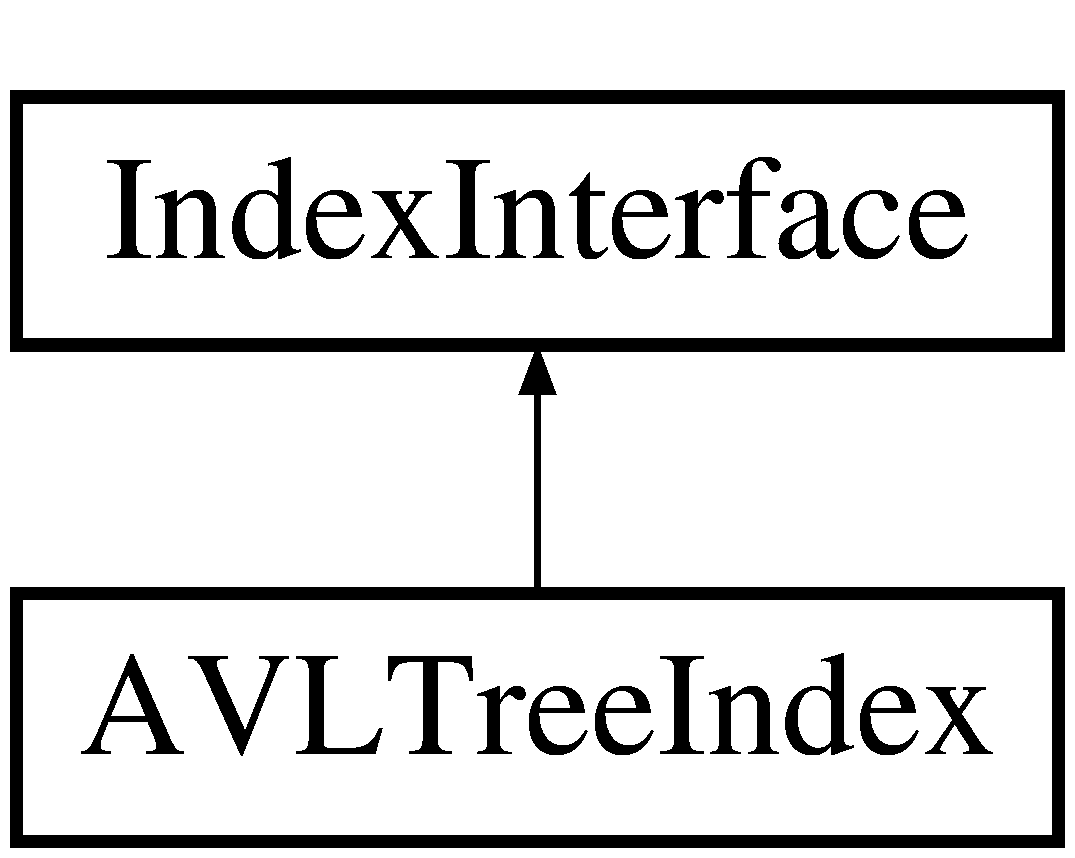
\includegraphics[height=2.000000cm]{class_a_v_l_tree_index}
\end{center}
\end{figure}
\subsection*{Public Member Functions}
\begin{DoxyCompactItemize}
\item 
\hyperlink{class_a_v_l_tree_index_aba8dc551ea4963a8082991f52bb19c25}{A\+V\+L\+Tree\+Index} ()
\begin{DoxyCompactList}\small\item\em Initializes the member data with default values. \end{DoxyCompactList}\item 
\hyperlink{class_a_v_l_tree_index_a33cfafc8516541f0d135c707955588f7}{$\sim$\+A\+V\+L\+Tree\+Index} ()
\begin{DoxyCompactList}\small\item\em Destructor for proper memory management. \end{DoxyCompactList}\item 
void \hyperlink{class_a_v_l_tree_index_a1f84720f7580bd785a11d0e0425bd537}{add\+Document} (const std\+::string \&path)
\begin{DoxyCompactList}\small\item\em Function for adding a document. \end{DoxyCompactList}\item 
void \hyperlink{class_a_v_l_tree_index_a1a877f264d30b657f37c6ed070d2e250}{clear\+Index} ()
\begin{DoxyCompactList}\small\item\em Function for clearing the index. \end{DoxyCompactList}\item 
bool \hyperlink{class_a_v_l_tree_index_a447e5741c289869d5a5188def065fb6c}{empty\+Index} () const 
\begin{DoxyCompactList}\small\item\em Function for returning whether the index is empty. \end{DoxyCompactList}\item 
\hyperlink{class_token}{Token} \hyperlink{class_a_v_l_tree_index_ab549fb6b9fdf08926540f6652859d442}{find\+Word} (std\+::string \&term)
\begin{DoxyCompactList}\small\item\em Function for finding a word in the index. \end{DoxyCompactList}\item 
const \hyperlink{class_document}{Document} \& \hyperlink{class_a_v_l_tree_index_a0716178493a342dd6b790cfa8d01b3fa}{get\+Document\+By\+I\+D} (const int \&doc\+I\+D)
\begin{DoxyCompactList}\small\item\em Function for getting a document pertaining to a given I\+D number. \end{DoxyCompactList}\item 
bool \hyperlink{class_a_v_l_tree_index_acb31068c39161358ec6545df5feaabc0}{has\+Word} (std\+::string \&term)
\begin{DoxyCompactList}\small\item\em Function for returning whether the index contains a given word. \end{DoxyCompactList}\item 
void \hyperlink{class_a_v_l_tree_index_a603741ace3489018f33f5ba4282e3f0d}{list\+Index} ()
\begin{DoxyCompactList}\small\item\em Function for writing the persistent index. \end{DoxyCompactList}\item 
bool \hyperlink{class_a_v_l_tree_index_af161b8697db7e3f599abc78a36f8d145}{load\+Index} ()
\begin{DoxyCompactList}\small\item\em Function for loading an index in from persistent state. \end{DoxyCompactList}\item 
bool \hyperlink{class_a_v_l_tree_index_a37200f167e48a7b24cb012b9ff5cf44c}{make\+Index} (const std\+::string \&file\+Name)
\begin{DoxyCompactList}\small\item\em Function for creating the index. \end{DoxyCompactList}\end{DoxyCompactItemize}


\subsection{Detailed Description}
Class for dealing with the index in A\+V\+L tree form. 

\begin{DoxySeeAlso}{See also}
\hyperlink{class_hash_table_index}{Hash\+Table\+Index}. 

\hyperlink{class_index_interface}{Index\+Interface}. 
\end{DoxySeeAlso}


\subsection{Constructor \& Destructor Documentation}
\hypertarget{class_a_v_l_tree_index_aba8dc551ea4963a8082991f52bb19c25}{}\index{A\+V\+L\+Tree\+Index@{A\+V\+L\+Tree\+Index}!A\+V\+L\+Tree\+Index@{A\+V\+L\+Tree\+Index}}
\index{A\+V\+L\+Tree\+Index@{A\+V\+L\+Tree\+Index}!A\+V\+L\+Tree\+Index@{A\+V\+L\+Tree\+Index}}
\subsubsection[{A\+V\+L\+Tree\+Index()}]{\setlength{\rightskip}{0pt plus 5cm}A\+V\+L\+Tree\+Index\+::\+A\+V\+L\+Tree\+Index (
\begin{DoxyParamCaption}
{}
\end{DoxyParamCaption}
)}\label{class_a_v_l_tree_index_aba8dc551ea4963a8082991f52bb19c25}


Initializes the member data with default values. 

\hypertarget{class_a_v_l_tree_index_a33cfafc8516541f0d135c707955588f7}{}\index{A\+V\+L\+Tree\+Index@{A\+V\+L\+Tree\+Index}!````~A\+V\+L\+Tree\+Index@{$\sim$\+A\+V\+L\+Tree\+Index}}
\index{````~A\+V\+L\+Tree\+Index@{$\sim$\+A\+V\+L\+Tree\+Index}!A\+V\+L\+Tree\+Index@{A\+V\+L\+Tree\+Index}}
\subsubsection[{$\sim$\+A\+V\+L\+Tree\+Index()}]{\setlength{\rightskip}{0pt plus 5cm}A\+V\+L\+Tree\+Index\+::$\sim$\+A\+V\+L\+Tree\+Index (
\begin{DoxyParamCaption}
{}
\end{DoxyParamCaption}
)}\label{class_a_v_l_tree_index_a33cfafc8516541f0d135c707955588f7}


Destructor for proper memory management. 



\subsection{Member Function Documentation}
\hypertarget{class_a_v_l_tree_index_a1f84720f7580bd785a11d0e0425bd537}{}\index{A\+V\+L\+Tree\+Index@{A\+V\+L\+Tree\+Index}!add\+Document@{add\+Document}}
\index{add\+Document@{add\+Document}!A\+V\+L\+Tree\+Index@{A\+V\+L\+Tree\+Index}}
\subsubsection[{add\+Document(const std\+::string \&path)}]{\setlength{\rightskip}{0pt plus 5cm}A\+V\+L\+Tree\+Index\+::add\+Document (
\begin{DoxyParamCaption}
\item[{const std\+::string \&}]{path}
\end{DoxyParamCaption}
)\hspace{0.3cm}{\ttfamily [virtual]}}\label{class_a_v_l_tree_index_a1f84720f7580bd785a11d0e0425bd537}


Function for adding a document. 


\begin{DoxyParams}{Parameters}
{\em path} & -\/ a path to a file to add to the index. \\
\hline
\end{DoxyParams}


Implements \hyperlink{class_index_interface_aa7601d76e8cc3f0657e800efdc4c127e}{Index\+Interface}.

\hypertarget{class_a_v_l_tree_index_a1a877f264d30b657f37c6ed070d2e250}{}\index{A\+V\+L\+Tree\+Index@{A\+V\+L\+Tree\+Index}!clear\+Index@{clear\+Index}}
\index{clear\+Index@{clear\+Index}!A\+V\+L\+Tree\+Index@{A\+V\+L\+Tree\+Index}}
\subsubsection[{clear\+Index()}]{\setlength{\rightskip}{0pt plus 5cm}A\+V\+L\+Tree\+Index\+::clear\+Index (
\begin{DoxyParamCaption}
{}
\end{DoxyParamCaption}
)\hspace{0.3cm}{\ttfamily [virtual]}}\label{class_a_v_l_tree_index_a1a877f264d30b657f37c6ed070d2e250}


Function for clearing the index. 



Implements \hyperlink{class_index_interface_aac36b4561598ee84c0c68958a1e3f82b}{Index\+Interface}.

\hypertarget{class_a_v_l_tree_index_a447e5741c289869d5a5188def065fb6c}{}\index{A\+V\+L\+Tree\+Index@{A\+V\+L\+Tree\+Index}!empty\+Index@{empty\+Index}}
\index{empty\+Index@{empty\+Index}!A\+V\+L\+Tree\+Index@{A\+V\+L\+Tree\+Index}}
\subsubsection[{empty\+Index() const }]{\setlength{\rightskip}{0pt plus 5cm}A\+V\+L\+Tree\+Index\+::empty\+Index (
\begin{DoxyParamCaption}
{}
\end{DoxyParamCaption}
) const\hspace{0.3cm}{\ttfamily [virtual]}}\label{class_a_v_l_tree_index_a447e5741c289869d5a5188def065fb6c}


Function for returning whether the index is empty. 

\begin{DoxyReturn}{Returns}
boolean whether the index is empty. 
\end{DoxyReturn}


Implements \hyperlink{class_index_interface_aaf90058a62e096bf607ea3dec2545ee4}{Index\+Interface}.

\hypertarget{class_a_v_l_tree_index_ab549fb6b9fdf08926540f6652859d442}{}\index{A\+V\+L\+Tree\+Index@{A\+V\+L\+Tree\+Index}!find\+Word@{find\+Word}}
\index{find\+Word@{find\+Word}!A\+V\+L\+Tree\+Index@{A\+V\+L\+Tree\+Index}}
\subsubsection[{find\+Word(std\+::string \&term)}]{\setlength{\rightskip}{0pt plus 5cm}A\+V\+L\+Tree\+Index\+::find\+Word (
\begin{DoxyParamCaption}
\item[{std\+::string \&}]{term}
\end{DoxyParamCaption}
)\hspace{0.3cm}{\ttfamily [virtual]}}\label{class_a_v_l_tree_index_ab549fb6b9fdf08926540f6652859d442}


Function for finding a word in the index. 


\begin{DoxyParams}{Parameters}
{\em term} & -\/ term to search for in the index. \\
\hline
\end{DoxyParams}
\begin{DoxyReturn}{Returns}
\hyperlink{class_token}{Token} (by value for \hyperlink{class_hash_table_index}{Hash\+Table\+Index} compatibility) representing the searched word. 
\end{DoxyReturn}


Implements \hyperlink{class_index_interface_aa0ea18e7daa9984240d108bd765b2816}{Index\+Interface}.

\hypertarget{class_a_v_l_tree_index_a0716178493a342dd6b790cfa8d01b3fa}{}\index{A\+V\+L\+Tree\+Index@{A\+V\+L\+Tree\+Index}!get\+Document\+By\+I\+D@{get\+Document\+By\+I\+D}}
\index{get\+Document\+By\+I\+D@{get\+Document\+By\+I\+D}!A\+V\+L\+Tree\+Index@{A\+V\+L\+Tree\+Index}}
\subsubsection[{get\+Document\+By\+I\+D(const int \&doc\+I\+D)}]{\setlength{\rightskip}{0pt plus 5cm}A\+V\+L\+Tree\+Index\+::get\+Document\+By\+I\+D (
\begin{DoxyParamCaption}
\item[{const int \&}]{doc\+I\+D}
\end{DoxyParamCaption}
)\hspace{0.3cm}{\ttfamily [virtual]}}\label{class_a_v_l_tree_index_a0716178493a342dd6b790cfa8d01b3fa}


Function for getting a document pertaining to a given I\+D number. 


\begin{DoxyParams}{Parameters}
{\em doc\+I\+D} & -\/ a document I\+D number. \\
\hline
\end{DoxyParams}
\begin{DoxyReturn}{Returns}
\hyperlink{class_document}{Document} reference. 
\end{DoxyReturn}


Implements \hyperlink{class_index_interface_aa694a3e8feb722519b45f7313281bfad}{Index\+Interface}.

\hypertarget{class_a_v_l_tree_index_acb31068c39161358ec6545df5feaabc0}{}\index{A\+V\+L\+Tree\+Index@{A\+V\+L\+Tree\+Index}!has\+Word@{has\+Word}}
\index{has\+Word@{has\+Word}!A\+V\+L\+Tree\+Index@{A\+V\+L\+Tree\+Index}}
\subsubsection[{has\+Word(std\+::string \&term)}]{\setlength{\rightskip}{0pt plus 5cm}A\+V\+L\+Tree\+Index\+::has\+Word (
\begin{DoxyParamCaption}
\item[{std\+::string \&}]{term}
\end{DoxyParamCaption}
)\hspace{0.3cm}{\ttfamily [virtual]}}\label{class_a_v_l_tree_index_acb31068c39161358ec6545df5feaabc0}


Function for returning whether the index contains a given word. 


\begin{DoxyParams}{Parameters}
{\em term} & -\/ a term to search the index for. \\
\hline
\end{DoxyParams}
\begin{DoxyReturn}{Returns}
boolean whether the index contains the word. 
\end{DoxyReturn}


Implements \hyperlink{class_index_interface_a8ccd80a03123406cb4b1e2494349f9da}{Index\+Interface}.

\hypertarget{class_a_v_l_tree_index_a603741ace3489018f33f5ba4282e3f0d}{}\index{A\+V\+L\+Tree\+Index@{A\+V\+L\+Tree\+Index}!list\+Index@{list\+Index}}
\index{list\+Index@{list\+Index}!A\+V\+L\+Tree\+Index@{A\+V\+L\+Tree\+Index}}
\subsubsection[{list\+Index()}]{\setlength{\rightskip}{0pt plus 5cm}A\+V\+L\+Tree\+Index\+::list\+Index (
\begin{DoxyParamCaption}
{}
\end{DoxyParamCaption}
)\hspace{0.3cm}{\ttfamily [virtual]}}\label{class_a_v_l_tree_index_a603741ace3489018f33f5ba4282e3f0d}


Function for writing the persistent index. 



Implements \hyperlink{class_index_interface_ad8567919eafa87ac20c35928c929084d}{Index\+Interface}.

\hypertarget{class_a_v_l_tree_index_af161b8697db7e3f599abc78a36f8d145}{}\index{A\+V\+L\+Tree\+Index@{A\+V\+L\+Tree\+Index}!load\+Index@{load\+Index}}
\index{load\+Index@{load\+Index}!A\+V\+L\+Tree\+Index@{A\+V\+L\+Tree\+Index}}
\subsubsection[{load\+Index()}]{\setlength{\rightskip}{0pt plus 5cm}A\+V\+L\+Tree\+Index\+::load\+Index (
\begin{DoxyParamCaption}
{}
\end{DoxyParamCaption}
)\hspace{0.3cm}{\ttfamily [virtual]}}\label{class_a_v_l_tree_index_af161b8697db7e3f599abc78a36f8d145}


Function for loading an index in from persistent state. 

\begin{DoxyReturn}{Returns}
boolean whether the index was successfully loaded. 
\end{DoxyReturn}


Implements \hyperlink{class_index_interface_a006f773f4e143745474e847cfb9f27fc}{Index\+Interface}.

\hypertarget{class_a_v_l_tree_index_a37200f167e48a7b24cb012b9ff5cf44c}{}\index{A\+V\+L\+Tree\+Index@{A\+V\+L\+Tree\+Index}!make\+Index@{make\+Index}}
\index{make\+Index@{make\+Index}!A\+V\+L\+Tree\+Index@{A\+V\+L\+Tree\+Index}}
\subsubsection[{make\+Index(const std\+::string \&file\+Name)}]{\setlength{\rightskip}{0pt plus 5cm}A\+V\+L\+Tree\+Index\+::make\+Index (
\begin{DoxyParamCaption}
\item[{const std\+::string \&}]{file\+Name}
\end{DoxyParamCaption}
)\hspace{0.3cm}{\ttfamily [virtual]}}\label{class_a_v_l_tree_index_a37200f167e48a7b24cb012b9ff5cf44c}


Function for creating the index. 


\begin{DoxyParams}{Parameters}
{\em file\+Name} & -\/ a directory containing files to be put in the index. \\
\hline
\end{DoxyParams}
\begin{DoxyReturn}{Returns}
boolean whether the index was successfully created. 
\end{DoxyReturn}


Implements \hyperlink{class_index_interface_a7b2ae510fa62eebb654708b90972c1b6}{Index\+Interface}.



The documentation for this class was generated from the following files\+:\begin{DoxyCompactItemize}
\item 
\hyperlink{_a_v_l_tree_index_8hpp}{A\+V\+L\+Tree\+Index.\+hpp}\item 
\hyperlink{_a_v_l_tree_index_8cpp}{A\+V\+L\+Tree\+Index.\+cpp}\end{DoxyCompactItemize}

\hypertarget{class_document}{}\section{Document Class Reference}
\label{class_document}\index{Document@{Document}}


Class for holding the information contained in a single page from Wiki\+Books.  




{\ttfamily \#include $<$Document.\+hpp$>$}

\subsection*{Public Member Functions}
\begin{DoxyCompactItemize}
\item 
\hyperlink{class_document_acdbcbe550084e8c20f4f67eb229ad66a}{Document} ()
\begin{DoxyCompactList}\small\item\em Initializes the member data with default values. \end{DoxyCompactList}\item 
\hyperlink{class_document_a37880d88667c09cc39ef46937f2cf6e4}{Document} (const std\+::string \&\hyperlink{class_document_a878497826a1ca34e778ef05f1a809d1a}{body}, const std\+::string \&\hyperlink{class_document_a1185d78c1c5c5ea69572c20d1c8e552a}{date}, const std\+::string \&\hyperlink{class_document_afda77c47efd90655ba5bb2ab8bf9ba00}{time}, const std\+::string \&\hyperlink{class_document_a4aac8266d0fea88e39ee390159130787}{title}, const std\+::string \&\hyperlink{class_document_a52990ba26536e2e3a08593444e0ccdf3}{username}, int \hyperlink{class_document_acda3a6caa3bc958024aa795cde6c7081}{id})
\item 
\hyperlink{class_document}{Document} \& \hyperlink{class_document_ad90511280d1b3815e57ed78003002ea1}{operator=} (const \hyperlink{class_document}{Document} \&copy)
\item 
const std\+::string \& \hyperlink{class_document_a878497826a1ca34e778ef05f1a809d1a}{body} () const 
\item 
void \hyperlink{class_document_a239171caccf983622b557898846c46e5}{body} (const std\+::string \&body)
\begin{DoxyCompactList}\small\item\em Sets the \hyperlink{class_document}{Document}\textquotesingle{}s body text. \end{DoxyCompactList}\item 
const std\+::string \& \hyperlink{class_document_a1185d78c1c5c5ea69572c20d1c8e552a}{date} () const 
\item 
void \hyperlink{class_document_a7e1af2cd6cb30c92b5f434863898019e}{date} (const std\+::string \&date)
\begin{DoxyCompactList}\small\item\em date the \hyperlink{class_document}{Document}\textquotesingle{}s date. \end{DoxyCompactList}\item 
const int \& \hyperlink{class_document_acda3a6caa3bc958024aa795cde6c7081}{id} () const 
\item 
void \hyperlink{class_document_ab538b0d75fd467eea80868917c63fbe5}{id} (const int \&id)
\begin{DoxyCompactList}\small\item\em Sets the \hyperlink{class_document}{Document}\textquotesingle{}s I\+D number. \end{DoxyCompactList}\item 
const std\+::string \& \hyperlink{class_document_afda77c47efd90655ba5bb2ab8bf9ba00}{time} () const 
\item 
void \hyperlink{class_document_a351642ea8074b80657d34a034797e53c}{time} (const std\+::string \&time)
\begin{DoxyCompactList}\small\item\em Sets the \hyperlink{class_document}{Document}\textquotesingle{}s time. \end{DoxyCompactList}\item 
const std\+::string \& \hyperlink{class_document_a4aac8266d0fea88e39ee390159130787}{title} () const 
\item 
void \hyperlink{class_document_ae586532a45e61a77afd0c0cfe95089ab}{title} (const std\+::string \&title)
\begin{DoxyCompactList}\small\item\em Sets the \hyperlink{class_document}{Document}\textquotesingle{}s title. \end{DoxyCompactList}\item 
const std\+::string \& \hyperlink{class_document_a52990ba26536e2e3a08593444e0ccdf3}{username} () const 
\item 
void \hyperlink{class_document_a24faf5e067badd65b55330535dec8c6a}{username} (const std\+::string \&username)
\begin{DoxyCompactList}\small\item\em Sets the \hyperlink{class_document}{Document}\textquotesingle{}s username. \end{DoxyCompactList}\end{DoxyCompactItemize}
\subsection*{Friends}
\begin{DoxyCompactItemize}
\item 
struct \hyperlink{class_document_ac81fac7a8d9ba85529addc5b3299f2ff}{std\+::hash$<$ Document $>$}
\item 
bool \hyperlink{class_document_ad4716fc286025a1c6b8020e517833e03}{operator==} (const \hyperlink{class_document}{Document} \&lhs, const \hyperlink{class_document}{Document} \&rhs)
\begin{DoxyCompactList}\small\item\em Compares two \hyperlink{class_document}{Document} objects for equality. \end{DoxyCompactList}\item 
bool \hyperlink{class_document_a333a5550c36ff69a94c749828fcf0165}{operator!=} (const \hyperlink{class_document}{Document} \&lhs, const \hyperlink{class_document}{Document} \&rhs)
\begin{DoxyCompactList}\small\item\em Compares two \hyperlink{class_document}{Document} objects for inequality. \end{DoxyCompactList}\item 
bool \hyperlink{class_document_a180fade9b73b45b1619be1e857b5b39e}{operator$<$} (const \hyperlink{class_document}{Document} \&lhs, const \hyperlink{class_document}{Document} \&rhs)
\begin{DoxyCompactList}\small\item\em Returns whether one \hyperlink{class_document}{Document} is less than another. \end{DoxyCompactList}\end{DoxyCompactItemize}


\subsection{Detailed Description}
Class for holding the information contained in a single page from Wiki\+Books. 

\begin{DoxySeeAlso}{See also}
\hyperlink{class_document_processor}{Document\+Processor}. 
\end{DoxySeeAlso}


\subsection{Constructor \& Destructor Documentation}
\hypertarget{class_document_acdbcbe550084e8c20f4f67eb229ad66a}{}\index{Document@{Document}!Document@{Document}}
\index{Document@{Document}!Document@{Document}}
\subsubsection[{Document()}]{\setlength{\rightskip}{0pt plus 5cm}Document\+::\+Document (
\begin{DoxyParamCaption}
{}
\end{DoxyParamCaption}
)\hspace{0.3cm}{\ttfamily [inline]}}\label{class_document_acdbcbe550084e8c20f4f67eb229ad66a}


Initializes the member data with default values. 

\hypertarget{class_document_a37880d88667c09cc39ef46937f2cf6e4}{}\index{Document@{Document}!Document@{Document}}
\index{Document@{Document}!Document@{Document}}
\subsubsection[{Document(const std\+::string \&body, const std\+::string \&date, const std\+::string \&time, const std\+::string \&title, const std\+::string \&username, int id)}]{\setlength{\rightskip}{0pt plus 5cm}Document\+::\+Document (
\begin{DoxyParamCaption}
\item[{const std\+::string \&}]{body, }
\item[{const std\+::string \&}]{date, }
\item[{const std\+::string \&}]{time, }
\item[{const std\+::string \&}]{title, }
\item[{const std\+::string \&}]{username, }
\item[{int}]{id}
\end{DoxyParamCaption}
)\hspace{0.3cm}{\ttfamily [inline]}}\label{class_document_a37880d88667c09cc39ef46937f2cf6e4}


\subsection{Member Function Documentation}
\hypertarget{class_document_a878497826a1ca34e778ef05f1a809d1a}{}\index{Document@{Document}!body@{body}}
\index{body@{body}!Document@{Document}}
\subsubsection[{body() const }]{\setlength{\rightskip}{0pt plus 5cm}const std\+::string\& Document\+::body (
\begin{DoxyParamCaption}
{}
\end{DoxyParamCaption}
) const\hspace{0.3cm}{\ttfamily [inline]}}\label{class_document_a878497826a1ca34e778ef05f1a809d1a}
\hypertarget{class_document_a239171caccf983622b557898846c46e5}{}\index{Document@{Document}!body@{body}}
\index{body@{body}!Document@{Document}}
\subsubsection[{body(const std\+::string \&body)}]{\setlength{\rightskip}{0pt plus 5cm}Document\+::body (
\begin{DoxyParamCaption}
\item[{const std\+::string \&}]{body}
\end{DoxyParamCaption}
)\hspace{0.3cm}{\ttfamily [inline]}}\label{class_document_a239171caccf983622b557898846c46e5}


Sets the \hyperlink{class_document}{Document}\textquotesingle{}s body text. 


\begin{DoxyParams}{Parameters}
{\em body} & -\/ a string to set the \hyperlink{class_document}{Document} body text to. \\
\hline
\end{DoxyParams}
\hypertarget{class_document_a1185d78c1c5c5ea69572c20d1c8e552a}{}\index{Document@{Document}!date@{date}}
\index{date@{date}!Document@{Document}}
\subsubsection[{date() const }]{\setlength{\rightskip}{0pt plus 5cm}const std\+::string\& Document\+::date (
\begin{DoxyParamCaption}
{}
\end{DoxyParamCaption}
) const\hspace{0.3cm}{\ttfamily [inline]}}\label{class_document_a1185d78c1c5c5ea69572c20d1c8e552a}
\hypertarget{class_document_a7e1af2cd6cb30c92b5f434863898019e}{}\index{Document@{Document}!date@{date}}
\index{date@{date}!Document@{Document}}
\subsubsection[{date(const std\+::string \&date)}]{\setlength{\rightskip}{0pt plus 5cm}Document\+::date (
\begin{DoxyParamCaption}
\item[{const std\+::string \&}]{date}
\end{DoxyParamCaption}
)\hspace{0.3cm}{\ttfamily [inline]}}\label{class_document_a7e1af2cd6cb30c92b5f434863898019e}


date the \hyperlink{class_document}{Document}\textquotesingle{}s date. 


\begin{DoxyParams}{Parameters}
{\em body} & -\/ a string to set the \hyperlink{class_document}{Document} date to. \\
\hline
\end{DoxyParams}
\hypertarget{class_document_acda3a6caa3bc958024aa795cde6c7081}{}\index{Document@{Document}!id@{id}}
\index{id@{id}!Document@{Document}}
\subsubsection[{id() const }]{\setlength{\rightskip}{0pt plus 5cm}const int\& Document\+::id (
\begin{DoxyParamCaption}
{}
\end{DoxyParamCaption}
) const\hspace{0.3cm}{\ttfamily [inline]}}\label{class_document_acda3a6caa3bc958024aa795cde6c7081}
\hypertarget{class_document_ab538b0d75fd467eea80868917c63fbe5}{}\index{Document@{Document}!id@{id}}
\index{id@{id}!Document@{Document}}
\subsubsection[{id(const int \&id)}]{\setlength{\rightskip}{0pt plus 5cm}Document\+::id (
\begin{DoxyParamCaption}
\item[{const int \&}]{id}
\end{DoxyParamCaption}
)\hspace{0.3cm}{\ttfamily [inline]}}\label{class_document_ab538b0d75fd467eea80868917c63fbe5}


Sets the \hyperlink{class_document}{Document}\textquotesingle{}s I\+D number. 


\begin{DoxyParams}{Parameters}
{\em id} & -\/ an integer to set the \hyperlink{class_document}{Document} I\+D to. \\
\hline
\end{DoxyParams}
\hypertarget{class_document_ad90511280d1b3815e57ed78003002ea1}{}\index{Document@{Document}!operator=@{operator=}}
\index{operator=@{operator=}!Document@{Document}}
\subsubsection[{operator=(const Document \&copy)}]{\setlength{\rightskip}{0pt plus 5cm}{\bf Document}\& Document\+::operator= (
\begin{DoxyParamCaption}
\item[{const {\bf Document} \&}]{copy}
\end{DoxyParamCaption}
)\hspace{0.3cm}{\ttfamily [inline]}}\label{class_document_ad90511280d1b3815e57ed78003002ea1}
\hypertarget{class_document_afda77c47efd90655ba5bb2ab8bf9ba00}{}\index{Document@{Document}!time@{time}}
\index{time@{time}!Document@{Document}}
\subsubsection[{time() const }]{\setlength{\rightskip}{0pt plus 5cm}const std\+::string\& Document\+::time (
\begin{DoxyParamCaption}
{}
\end{DoxyParamCaption}
) const\hspace{0.3cm}{\ttfamily [inline]}}\label{class_document_afda77c47efd90655ba5bb2ab8bf9ba00}
\hypertarget{class_document_a351642ea8074b80657d34a034797e53c}{}\index{Document@{Document}!time@{time}}
\index{time@{time}!Document@{Document}}
\subsubsection[{time(const std\+::string \&time)}]{\setlength{\rightskip}{0pt plus 5cm}Document\+::time (
\begin{DoxyParamCaption}
\item[{const std\+::string \&}]{time}
\end{DoxyParamCaption}
)\hspace{0.3cm}{\ttfamily [inline]}}\label{class_document_a351642ea8074b80657d34a034797e53c}


Sets the \hyperlink{class_document}{Document}\textquotesingle{}s time. 


\begin{DoxyParams}{Parameters}
{\em time} & -\/ a string to set the \hyperlink{class_document}{Document} time to. \\
\hline
\end{DoxyParams}
\hypertarget{class_document_a4aac8266d0fea88e39ee390159130787}{}\index{Document@{Document}!title@{title}}
\index{title@{title}!Document@{Document}}
\subsubsection[{title() const }]{\setlength{\rightskip}{0pt plus 5cm}const std\+::string\& Document\+::title (
\begin{DoxyParamCaption}
{}
\end{DoxyParamCaption}
) const\hspace{0.3cm}{\ttfamily [inline]}}\label{class_document_a4aac8266d0fea88e39ee390159130787}
\hypertarget{class_document_ae586532a45e61a77afd0c0cfe95089ab}{}\index{Document@{Document}!title@{title}}
\index{title@{title}!Document@{Document}}
\subsubsection[{title(const std\+::string \&title)}]{\setlength{\rightskip}{0pt plus 5cm}Document\+::title (
\begin{DoxyParamCaption}
\item[{const std\+::string \&}]{title}
\end{DoxyParamCaption}
)\hspace{0.3cm}{\ttfamily [inline]}}\label{class_document_ae586532a45e61a77afd0c0cfe95089ab}


Sets the \hyperlink{class_document}{Document}\textquotesingle{}s title. 


\begin{DoxyParams}{Parameters}
{\em title} & -\/ a string to set the \hyperlink{class_document}{Document} title to. \\
\hline
\end{DoxyParams}
\hypertarget{class_document_a52990ba26536e2e3a08593444e0ccdf3}{}\index{Document@{Document}!username@{username}}
\index{username@{username}!Document@{Document}}
\subsubsection[{username() const }]{\setlength{\rightskip}{0pt plus 5cm}const std\+::string\& Document\+::username (
\begin{DoxyParamCaption}
{}
\end{DoxyParamCaption}
) const\hspace{0.3cm}{\ttfamily [inline]}}\label{class_document_a52990ba26536e2e3a08593444e0ccdf3}
\hypertarget{class_document_a24faf5e067badd65b55330535dec8c6a}{}\index{Document@{Document}!username@{username}}
\index{username@{username}!Document@{Document}}
\subsubsection[{username(const std\+::string \&username)}]{\setlength{\rightskip}{0pt plus 5cm}Document\+::username (
\begin{DoxyParamCaption}
\item[{const std\+::string \&}]{username}
\end{DoxyParamCaption}
)\hspace{0.3cm}{\ttfamily [inline]}}\label{class_document_a24faf5e067badd65b55330535dec8c6a}


Sets the \hyperlink{class_document}{Document}\textquotesingle{}s username. 


\begin{DoxyParams}{Parameters}
{\em username} & -\/ a string to set the \hyperlink{class_document}{Document} username to. \\
\hline
\end{DoxyParams}


\subsection{Friends And Related Function Documentation}
\hypertarget{class_document_a333a5550c36ff69a94c749828fcf0165}{}\index{Document@{Document}!operator"!=@{operator"!=}}
\index{operator"!=@{operator"!=}!Document@{Document}}
\subsubsection[{operator"!=}]{\setlength{\rightskip}{0pt plus 5cm}Document\+::operator!= (
\begin{DoxyParamCaption}
\item[{const {\bf Document} \&}]{lhs, }
\item[{const {\bf Document} \&}]{rhs}
\end{DoxyParamCaption}
)\hspace{0.3cm}{\ttfamily [friend]}}\label{class_document_a333a5550c36ff69a94c749828fcf0165}


Compares two \hyperlink{class_document}{Document} objects for inequality. 


\begin{DoxyParams}{Parameters}
{\em lhs} & -\/ A constant \hyperlink{class_document}{Document} reference. \\
\hline
{\em rhs} & -\/ A constant \hyperlink{class_document}{Document} reference. \\
\hline
\end{DoxyParams}
\begin{DoxyReturn}{Returns}
boolean whether two Tokens are not the same. 
\end{DoxyReturn}
\hypertarget{class_document_a180fade9b73b45b1619be1e857b5b39e}{}\index{Document@{Document}!operator$<$@{operator$<$}}
\index{operator$<$@{operator$<$}!Document@{Document}}
\subsubsection[{operator$<$}]{\setlength{\rightskip}{0pt plus 5cm}Document\+::operator$<$ (
\begin{DoxyParamCaption}
\item[{const {\bf Document} \&}]{lhs, }
\item[{const {\bf Document} \&}]{rhs}
\end{DoxyParamCaption}
)\hspace{0.3cm}{\ttfamily [friend]}}\label{class_document_a180fade9b73b45b1619be1e857b5b39e}


Returns whether one \hyperlink{class_document}{Document} is less than another. 


\begin{DoxyParams}{Parameters}
{\em lhs} & -\/ A constant \hyperlink{class_document}{Document} reference. \\
\hline
{\em rhs} & -\/ A constant \hyperlink{class_document}{Document} reference. \\
\hline
\end{DoxyParams}
\begin{DoxyReturn}{Returns}
boolean whether one \hyperlink{class_token}{Token} is less than another. 
\end{DoxyReturn}
\hypertarget{class_document_ad4716fc286025a1c6b8020e517833e03}{}\index{Document@{Document}!operator==@{operator==}}
\index{operator==@{operator==}!Document@{Document}}
\subsubsection[{operator==}]{\setlength{\rightskip}{0pt plus 5cm}Document\+::operator== (
\begin{DoxyParamCaption}
\item[{const {\bf Document} \&}]{lhs, }
\item[{const {\bf Document} \&}]{rhs}
\end{DoxyParamCaption}
)\hspace{0.3cm}{\ttfamily [friend]}}\label{class_document_ad4716fc286025a1c6b8020e517833e03}


Compares two \hyperlink{class_document}{Document} objects for equality. 


\begin{DoxyParams}{Parameters}
{\em lhs} & -\/ A constant \hyperlink{class_document}{Document} reference. \\
\hline
{\em rhs} & -\/ A constant \hyperlink{class_document}{Document} reference. \\
\hline
\end{DoxyParams}
\begin{DoxyReturn}{Returns}
boolean whether two Tokens are the same. 
\end{DoxyReturn}
\hypertarget{class_document_ac81fac7a8d9ba85529addc5b3299f2ff}{}\index{Document@{Document}!std\+::hash$<$ Document $>$@{std\+::hash$<$ Document $>$}}
\index{std\+::hash$<$ Document $>$@{std\+::hash$<$ Document $>$}!Document@{Document}}
\subsubsection[{std\+::hash$<$ Document $>$}]{\setlength{\rightskip}{0pt plus 5cm}friend struct std\+::hash$<$ {\bf Document} $>$\hspace{0.3cm}{\ttfamily [friend]}}\label{class_document_ac81fac7a8d9ba85529addc5b3299f2ff}


The documentation for this class was generated from the following file\+:\begin{DoxyCompactItemize}
\item 
\hyperlink{_document_8hpp}{Document.\+hpp}\end{DoxyCompactItemize}

\hypertarget{class_document_processor}{}\section{Document\+Processor Class Reference}
\label{class_document_processor}\index{Document\+Processor@{Document\+Processor}}


Processes each document from the corpus.  




{\ttfamily \#include $<$Document\+Processor.\+hpp$>$}

\subsection*{Public Member Functions}
\begin{DoxyCompactItemize}
\item 
\hyperlink{class_document_processor_a4a4cefc8163b834855aa0cd0aec68d86}{Document\+Processor} ()
\begin{DoxyCompactList}\small\item\em Loads the stopwords into the std\+::unordered\+\_\+set by default. \end{DoxyCompactList}\item 
bool \hyperlink{class_document_processor_aa04641c8135b87e07ccb2b73283938ba}{add\+Document} (const std\+::string \&file\+Name, \hyperlink{class_a_v_l_tree}{A\+V\+L\+Tree}$<$ \hyperlink{class_token}{Token} $>$ \&tokens)
\begin{DoxyCompactList}\small\item\em Adds a document to the set of documents. \end{DoxyCompactList}\item 
bool \hyperlink{class_document_processor_a3f1563705a88a8ab9ea63af0a929917c}{add\+Document} (const std\+::string \&file\+Name, index\+\_\+type \&index)
\begin{DoxyCompactList}\small\item\em Adds a document to the set of documents. \end{DoxyCompactList}\item 
bool \hyperlink{class_document_processor_a9fc30d3b7c2220c86cd4b672c512b109}{batch\+Tokenize} (const std\+::string \&file\+Name, \hyperlink{class_a_v_l_tree}{A\+V\+L\+Tree}$<$ \hyperlink{class_token}{Token} $>$ \&tokens)
\begin{DoxyCompactList}\small\item\em Parses the X\+M\+L file(s), tokenizes the pages, and adds each \hyperlink{class_token}{Token} to the A\+V\+L tree. \end{DoxyCompactList}\item 
bool \hyperlink{class_document_processor_a19db4cd4e6367bbbd51fb6b6b1ea8396}{batch\+Tokenize} (const std\+::string \&file\+Name, index\+\_\+type \&index)
\begin{DoxyCompactList}\small\item\em Parses the X\+M\+L file(s), tokenizes the pages, and adds each token to the index. \end{DoxyCompactList}\item 
void \hyperlink{class_document_processor_a126fc41f4a3ec8af3240714862e686c5}{clear} ()
\begin{DoxyCompactList}\small\item\em Clears the contents of the set of documents. \end{DoxyCompactList}\item 
bool \hyperlink{class_document_processor_a0ca26f0de7652ae68da6ad06673b2304}{create\+Documents} (const std\+::string \&file\+Name)
\item 
int \hyperlink{class_document_processor_a09d1b766a653de2d1ce6a81f2213d975}{documents\+Size} () const 
\begin{DoxyCompactList}\small\item\em Returns the number of documents processed. \end{DoxyCompactList}\item 
std\+::unordered\+\_\+set$<$ \hyperlink{class_document}{Document} $>$ \& \hyperlink{class_document_processor_a7e0fff87749449ff712fab6deed57e8e}{get\+Documents} ()
\begin{DoxyCompactList}\small\item\em Returns the set of Documents. \end{DoxyCompactList}\item 
const \hyperlink{class_document}{Document} \& \hyperlink{class_document_processor_a3f725ffc320008889f9a2797b8dadb70}{get\+Document\+By\+I\+D} (const int \&doc\+I\+D)
\begin{DoxyCompactList}\small\item\em Returns a specific document out of the set pertaining to a specific I\+D number. \end{DoxyCompactList}\item 
void \hyperlink{class_document_processor_a2efd77c307ac1672d77b582be3cf57f9}{tokenize} (\hyperlink{class_document}{Document} \&doc, \hyperlink{class_a_v_l_tree}{A\+V\+L\+Tree}$<$ \hyperlink{class_token}{Token} $>$ \&tokens)
\begin{DoxyCompactList}\small\item\em Tokenizes a given \hyperlink{class_document}{Document} and adds the Tokens to the given A\+V\+L tree. \end{DoxyCompactList}\item 
void \hyperlink{class_document_processor_ab83334ce4255441e2757dc39cdbbd1ed}{tokenize} (\hyperlink{class_document}{Document} \&doc, index\+\_\+type \&index)
\begin{DoxyCompactList}\small\item\em Tokenizes a given \hyperlink{class_document}{Document} and adds the tokens to the index. \end{DoxyCompactList}\end{DoxyCompactItemize}


\subsection{Detailed Description}
Processes each document from the corpus. 

Stems and removes stop words. Computes term frequencies (information stored in \hyperlink{class_token}{Token} objects) \begin{DoxySeeAlso}{See also}
\hyperlink{class_document}{Document}. 

\hyperlink{class_token}{Token}. 
\end{DoxySeeAlso}


\subsection{Constructor \& Destructor Documentation}
\hypertarget{class_document_processor_a4a4cefc8163b834855aa0cd0aec68d86}{}\index{Document\+Processor@{Document\+Processor}!Document\+Processor@{Document\+Processor}}
\index{Document\+Processor@{Document\+Processor}!Document\+Processor@{Document\+Processor}}
\subsubsection[{Document\+Processor()}]{\setlength{\rightskip}{0pt plus 5cm}Document\+Processor\+::\+Document\+Processor (
\begin{DoxyParamCaption}
{}
\end{DoxyParamCaption}
)}\label{class_document_processor_a4a4cefc8163b834855aa0cd0aec68d86}


Loads the stopwords into the std\+::unordered\+\_\+set by default. 



\subsection{Member Function Documentation}
\hypertarget{class_document_processor_aa04641c8135b87e07ccb2b73283938ba}{}\index{Document\+Processor@{Document\+Processor}!add\+Document@{add\+Document}}
\index{add\+Document@{add\+Document}!Document\+Processor@{Document\+Processor}}
\subsubsection[{add\+Document(const std\+::string \&file\+Name, A\+V\+L\+Tree$<$ Token $>$ \&tokens)}]{\setlength{\rightskip}{0pt plus 5cm}Document\+Processor\+::add\+Document (
\begin{DoxyParamCaption}
\item[{const std\+::string \&}]{file\+Name, }
\item[{{\bf A\+V\+L\+Tree}$<$ {\bf Token} $>$ \&}]{tokens}
\end{DoxyParamCaption}
)}\label{class_document_processor_aa04641c8135b87e07ccb2b73283938ba}


Adds a document to the set of documents. 


\begin{DoxyParams}{Parameters}
{\em file\+Name} & -\/ a string representing the path to the file to parse. \\
\hline
{\em tokens} & -\/ an A\+V\+L tree that holds the resulting tokens. \\
\hline
\end{DoxyParams}
\begin{DoxyReturn}{Returns}
boolean whether the document was added successfully. 
\end{DoxyReturn}
\hypertarget{class_document_processor_a3f1563705a88a8ab9ea63af0a929917c}{}\index{Document\+Processor@{Document\+Processor}!add\+Document@{add\+Document}}
\index{add\+Document@{add\+Document}!Document\+Processor@{Document\+Processor}}
\subsubsection[{add\+Document(const std\+::string \&file\+Name, index\+\_\+type \&index)}]{\setlength{\rightskip}{0pt plus 5cm}Document\+Processor\+::add\+Document (
\begin{DoxyParamCaption}
\item[{const std\+::string \&}]{file\+Name, }
\item[{index\+\_\+type \&}]{index}
\end{DoxyParamCaption}
)}\label{class_document_processor_a3f1563705a88a8ab9ea63af0a929917c}


Adds a document to the set of documents. 


\begin{DoxyParams}{Parameters}
{\em file\+Name} & -\/ a string representing the path to the file to parse. \\
\hline
{\em index} & -\/ an index object that holds the resulting data. \\
\hline
\end{DoxyParams}
\begin{DoxyReturn}{Returns}
boolean whether the document was added successfully. 
\end{DoxyReturn}
\hypertarget{class_document_processor_a9fc30d3b7c2220c86cd4b672c512b109}{}\index{Document\+Processor@{Document\+Processor}!batch\+Tokenize@{batch\+Tokenize}}
\index{batch\+Tokenize@{batch\+Tokenize}!Document\+Processor@{Document\+Processor}}
\subsubsection[{batch\+Tokenize(const std\+::string \&file\+Name, A\+V\+L\+Tree$<$ Token $>$ \&tokens)}]{\setlength{\rightskip}{0pt plus 5cm}Document\+Processor\+::batch\+Tokenize (
\begin{DoxyParamCaption}
\item[{const std\+::string \&}]{path, }
\item[{{\bf A\+V\+L\+Tree}$<$ {\bf Token} $>$ \&}]{tokens}
\end{DoxyParamCaption}
)}\label{class_document_processor_a9fc30d3b7c2220c86cd4b672c512b109}


Parses the X\+M\+L file(s), tokenizes the pages, and adds each \hyperlink{class_token}{Token} to the A\+V\+L tree. 


\begin{DoxyParams}{Parameters}
{\em path} & -\/ a path to the directory containing the file(s). \\
\hline
{\em tokens} & -\/ an A\+V\+L tree that holds the resulting tokens. \\
\hline
\end{DoxyParams}
\begin{DoxyReturn}{Returns}
boolean whether the process was successful. 
\end{DoxyReturn}
\hypertarget{class_document_processor_a19db4cd4e6367bbbd51fb6b6b1ea8396}{}\index{Document\+Processor@{Document\+Processor}!batch\+Tokenize@{batch\+Tokenize}}
\index{batch\+Tokenize@{batch\+Tokenize}!Document\+Processor@{Document\+Processor}}
\subsubsection[{batch\+Tokenize(const std\+::string \&file\+Name, index\+\_\+type \&index)}]{\setlength{\rightskip}{0pt plus 5cm}Document\+Processor\+::batch\+Tokenize (
\begin{DoxyParamCaption}
\item[{const std\+::string \&}]{path, }
\item[{index\+\_\+type \&}]{index}
\end{DoxyParamCaption}
)}\label{class_document_processor_a19db4cd4e6367bbbd51fb6b6b1ea8396}


Parses the X\+M\+L file(s), tokenizes the pages, and adds each token to the index. 


\begin{DoxyParams}{Parameters}
{\em path} & -\/ a path to the directory containing the file(s). \\
\hline
{\em index} & -\/ an index object that holds the resulting data \\
\hline
\end{DoxyParams}
\begin{DoxyReturn}{Returns}
boolean whether the process was successful. 
\end{DoxyReturn}
\hypertarget{class_document_processor_a126fc41f4a3ec8af3240714862e686c5}{}\index{Document\+Processor@{Document\+Processor}!clear@{clear}}
\index{clear@{clear}!Document\+Processor@{Document\+Processor}}
\subsubsection[{clear()}]{\setlength{\rightskip}{0pt plus 5cm}Document\+Processor\+::clear (
\begin{DoxyParamCaption}
{}
\end{DoxyParamCaption}
)}\label{class_document_processor_a126fc41f4a3ec8af3240714862e686c5}


Clears the contents of the set of documents. 

\hypertarget{class_document_processor_a0ca26f0de7652ae68da6ad06673b2304}{}\index{Document\+Processor@{Document\+Processor}!create\+Documents@{create\+Documents}}
\index{create\+Documents@{create\+Documents}!Document\+Processor@{Document\+Processor}}
\subsubsection[{create\+Documents(const std\+::string \&file\+Name)}]{\setlength{\rightskip}{0pt plus 5cm}bool Document\+Processor\+::create\+Documents (
\begin{DoxyParamCaption}
\item[{const std\+::string \&}]{file\+Name}
\end{DoxyParamCaption}
)}\label{class_document_processor_a0ca26f0de7652ae68da6ad06673b2304}
\hypertarget{class_document_processor_a09d1b766a653de2d1ce6a81f2213d975}{}\index{Document\+Processor@{Document\+Processor}!documents\+Size@{documents\+Size}}
\index{documents\+Size@{documents\+Size}!Document\+Processor@{Document\+Processor}}
\subsubsection[{documents\+Size() const }]{\setlength{\rightskip}{0pt plus 5cm}Document\+Processor\+::documents\+Size (
\begin{DoxyParamCaption}
{}
\end{DoxyParamCaption}
) const}\label{class_document_processor_a09d1b766a653de2d1ce6a81f2213d975}


Returns the number of documents processed. 

\begin{DoxyReturn}{Returns}
integer representing the number of documents processed. 
\end{DoxyReturn}
\hypertarget{class_document_processor_a3f725ffc320008889f9a2797b8dadb70}{}\index{Document\+Processor@{Document\+Processor}!get\+Document\+By\+I\+D@{get\+Document\+By\+I\+D}}
\index{get\+Document\+By\+I\+D@{get\+Document\+By\+I\+D}!Document\+Processor@{Document\+Processor}}
\subsubsection[{get\+Document\+By\+I\+D(const int \&doc\+I\+D)}]{\setlength{\rightskip}{0pt plus 5cm}Document\+Processor\+::get\+Document\+By\+I\+D (
\begin{DoxyParamCaption}
\item[{const int \&}]{doc\+I\+D}
\end{DoxyParamCaption}
)}\label{class_document_processor_a3f725ffc320008889f9a2797b8dadb70}


Returns a specific document out of the set pertaining to a specific I\+D number. 

\begin{DoxyReturn}{Returns}
const \hyperlink{class_document}{Document} reference pertaining to the given I\+D number. 
\end{DoxyReturn}
\hypertarget{class_document_processor_a7e0fff87749449ff712fab6deed57e8e}{}\index{Document\+Processor@{Document\+Processor}!get\+Documents@{get\+Documents}}
\index{get\+Documents@{get\+Documents}!Document\+Processor@{Document\+Processor}}
\subsubsection[{get\+Documents()}]{\setlength{\rightskip}{0pt plus 5cm}Document\+Processor\+::get\+Documents (
\begin{DoxyParamCaption}
{}
\end{DoxyParamCaption}
)}\label{class_document_processor_a7e0fff87749449ff712fab6deed57e8e}


Returns the set of Documents. 

\begin{DoxyReturn}{Returns}
std\+::unordered\+\_\+set containing the documents. 
\end{DoxyReturn}
\hypertarget{class_document_processor_a2efd77c307ac1672d77b582be3cf57f9}{}\index{Document\+Processor@{Document\+Processor}!tokenize@{tokenize}}
\index{tokenize@{tokenize}!Document\+Processor@{Document\+Processor}}
\subsubsection[{tokenize(\+Document \&doc, A\+V\+L\+Tree$<$ Token $>$ \&tokens)}]{\setlength{\rightskip}{0pt plus 5cm}Document\+Processor\+::tokenize (
\begin{DoxyParamCaption}
\item[{{\bf Document} \&}]{doc, }
\item[{{\bf A\+V\+L\+Tree}$<$ {\bf Token} $>$ \&}]{tokens}
\end{DoxyParamCaption}
)}\label{class_document_processor_a2efd77c307ac1672d77b582be3cf57f9}


Tokenizes a given \hyperlink{class_document}{Document} and adds the Tokens to the given A\+V\+L tree. 


\begin{DoxyParams}{Parameters}
{\em doc} & -\/ a document to tokenize. \\
\hline
{\em tokens} & -\/ an A\+V\+L tree that holds the resulting tokens. \\
\hline
\end{DoxyParams}
\hypertarget{class_document_processor_ab83334ce4255441e2757dc39cdbbd1ed}{}\index{Document\+Processor@{Document\+Processor}!tokenize@{tokenize}}
\index{tokenize@{tokenize}!Document\+Processor@{Document\+Processor}}
\subsubsection[{tokenize(\+Document \&doc, index\+\_\+type \&index)}]{\setlength{\rightskip}{0pt plus 5cm}Document\+Processor\+::tokenize (
\begin{DoxyParamCaption}
\item[{{\bf Document} \&}]{doc, }
\item[{index\+\_\+type \&}]{tokens}
\end{DoxyParamCaption}
)}\label{class_document_processor_ab83334ce4255441e2757dc39cdbbd1ed}


Tokenizes a given \hyperlink{class_document}{Document} and adds the tokens to the index. 


\begin{DoxyParams}{Parameters}
{\em doc} & -\/ a document to tokenize. \\
\hline
{\em index} & -\/ an index object that holds the resulting data. \\
\hline
\end{DoxyParams}


The documentation for this class was generated from the following files\+:\begin{DoxyCompactItemize}
\item 
\hyperlink{_document_processor_8hpp}{Document\+Processor.\+hpp}\item 
\hyperlink{_document_processor_8cpp}{Document\+Processor.\+cpp}\end{DoxyCompactItemize}

\hypertarget{structstd_1_1std_1_1hash_3_01_document_01_4}{}\section{std\+:\+:std\+:\+:hash$<$ Document $>$ Struct Template Reference}
\label{structstd_1_1std_1_1hash_3_01_document_01_4}\index{std\+::std\+::hash$<$ Document $>$@{std\+::std\+::hash$<$ Document $>$}}


{\ttfamily \#include $<$Document.\+hpp$>$}

\subsection*{Public Member Functions}
\begin{DoxyCompactItemize}
\item 
std\+::size\+\_\+t \hyperlink{structstd_1_1std_1_1hash_3_01_document_01_4_a093cc76d99ae61bbc7e21c1e6244d0ed}{operator()} (const \hyperlink{class_document}{Document} \&doc)
\end{DoxyCompactItemize}


\subsection{Member Function Documentation}
\hypertarget{structstd_1_1std_1_1hash_3_01_document_01_4_a093cc76d99ae61bbc7e21c1e6244d0ed}{}\index{std\+::std\+::hash$<$ Document $>$@{std\+::std\+::hash$<$ Document $>$}!operator()@{operator()}}
\index{operator()@{operator()}!std\+::std\+::hash$<$ Document $>$@{std\+::std\+::hash$<$ Document $>$}}
\subsubsection[{operator()(const Document \&doc)}]{\setlength{\rightskip}{0pt plus 5cm}std\+::size\+\_\+t std\+::std\+::hash$<$ {\bf Document} $>$\+::operator() (
\begin{DoxyParamCaption}
\item[{const {\bf Document} \&}]{doc}
\end{DoxyParamCaption}
)\hspace{0.3cm}{\ttfamily [inline]}}\label{structstd_1_1std_1_1hash_3_01_document_01_4_a093cc76d99ae61bbc7e21c1e6244d0ed}


The documentation for this struct was generated from the following file\+:\begin{DoxyCompactItemize}
\item 
\hyperlink{_document_8hpp}{Document.\+hpp}\end{DoxyCompactItemize}

\hypertarget{class_hash_table_index}{}\section{Hash\+Table\+Index Class Reference}
\label{class_hash_table_index}\index{Hash\+Table\+Index@{Hash\+Table\+Index}}


Class for dealing with the index in hash table form.  




{\ttfamily \#include $<$Hash\+Table\+Index.\+hpp$>$}

Inheritance diagram for Hash\+Table\+Index\+:\begin{figure}[H]
\begin{center}
\leavevmode
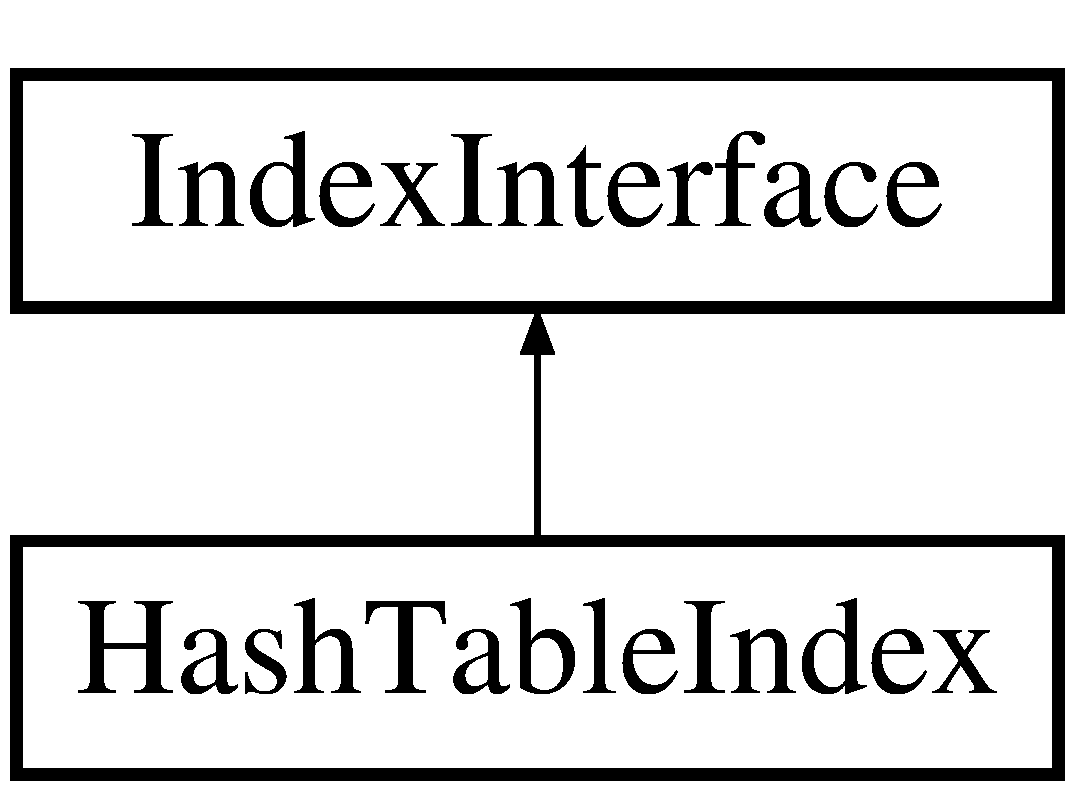
\includegraphics[height=2.000000cm]{class_hash_table_index}
\end{center}
\end{figure}
\subsection*{Public Member Functions}
\begin{DoxyCompactItemize}
\item 
\hyperlink{class_hash_table_index_a13c1c8deae84226c8bef382adf103b53}{Hash\+Table\+Index} ()
\begin{DoxyCompactList}\small\item\em Initializes the member data with default values. \end{DoxyCompactList}\item 
\hyperlink{class_hash_table_index_af4d2eeae8263c353f91140cb2583fb58}{$\sim$\+Hash\+Table\+Index} ()
\begin{DoxyCompactList}\small\item\em Destructor for proper memory management of this and child classes. \end{DoxyCompactList}\item 
void \hyperlink{class_hash_table_index_a5387a8b9f0e585105a79624a93cd6ec0}{add\+Document} (const std\+::string \&path)
\begin{DoxyCompactList}\small\item\em Function for adding a document. \end{DoxyCompactList}\item 
void \hyperlink{class_hash_table_index_a69b31cc0bb54877b628bd67dadc5973f}{clear\+Index} ()
\begin{DoxyCompactList}\small\item\em Function for clearing the index. \end{DoxyCompactList}\item 
bool \hyperlink{class_hash_table_index_a19b62a531429e670b25cd92be4333890}{empty\+Index} () const 
\begin{DoxyCompactList}\small\item\em Function for returning whether the index is empty. \end{DoxyCompactList}\item 
\hyperlink{class_token}{Token} \hyperlink{class_hash_table_index_a3d4c8e0244943cc44f33a35b742f7578}{find\+Word} (std\+::string \&term)
\begin{DoxyCompactList}\small\item\em Function for finding a word in the index. \end{DoxyCompactList}\item 
const \hyperlink{class_document}{Document} \& \hyperlink{class_hash_table_index_ac5cc9451bce6e13739af7c5f154eea0b}{get\+Document\+By\+I\+D} (const int \&doc\+I\+D)
\begin{DoxyCompactList}\small\item\em Function for getting a document pertaining to a given I\+D number. \end{DoxyCompactList}\item 
bool \hyperlink{class_hash_table_index_aea9366ff9299d41bd3447bc6c95a3960}{has\+Word} (std\+::string \&term)
\begin{DoxyCompactList}\small\item\em Function for returning whether the index contains a given word. \end{DoxyCompactList}\item 
void \hyperlink{class_hash_table_index_a42bbd9b325fb95b54a546c3c98c67624}{list\+Index} ()
\begin{DoxyCompactList}\small\item\em Function for writing the persistent index. \end{DoxyCompactList}\item 
bool \hyperlink{class_hash_table_index_a8c483a83b40b49b0f35be9fea0674501}{load\+Index} ()
\begin{DoxyCompactList}\small\item\em Function for loading an index in from persistent state. \end{DoxyCompactList}\item 
bool \hyperlink{class_hash_table_index_a5105f715d8c5fd3b74d6bec462cb0c38}{make\+Index} (const std\+::string \&file\+Name)
\begin{DoxyCompactList}\small\item\em Function for creating the index. \end{DoxyCompactList}\end{DoxyCompactItemize}


\subsection{Detailed Description}
Class for dealing with the index in hash table form. 

\begin{DoxySeeAlso}{See also}
\hyperlink{class_a_v_l_tree_index}{A\+V\+L\+Tree\+Index}. 

\hyperlink{class_index_interface}{Index\+Interface}. 
\end{DoxySeeAlso}


\subsection{Constructor \& Destructor Documentation}
\hypertarget{class_hash_table_index_a13c1c8deae84226c8bef382adf103b53}{}\index{Hash\+Table\+Index@{Hash\+Table\+Index}!Hash\+Table\+Index@{Hash\+Table\+Index}}
\index{Hash\+Table\+Index@{Hash\+Table\+Index}!Hash\+Table\+Index@{Hash\+Table\+Index}}
\subsubsection[{Hash\+Table\+Index()}]{\setlength{\rightskip}{0pt plus 5cm}Hash\+Table\+Index\+::\+Hash\+Table\+Index (
\begin{DoxyParamCaption}
{}
\end{DoxyParamCaption}
)}\label{class_hash_table_index_a13c1c8deae84226c8bef382adf103b53}


Initializes the member data with default values. 

\hypertarget{class_hash_table_index_af4d2eeae8263c353f91140cb2583fb58}{}\index{Hash\+Table\+Index@{Hash\+Table\+Index}!````~Hash\+Table\+Index@{$\sim$\+Hash\+Table\+Index}}
\index{````~Hash\+Table\+Index@{$\sim$\+Hash\+Table\+Index}!Hash\+Table\+Index@{Hash\+Table\+Index}}
\subsubsection[{$\sim$\+Hash\+Table\+Index()}]{\setlength{\rightskip}{0pt plus 5cm}Hash\+Table\+Index\+::$\sim$\+Hash\+Table\+Index (
\begin{DoxyParamCaption}
{}
\end{DoxyParamCaption}
)}\label{class_hash_table_index_af4d2eeae8263c353f91140cb2583fb58}


Destructor for proper memory management of this and child classes. 



\subsection{Member Function Documentation}
\hypertarget{class_hash_table_index_a5387a8b9f0e585105a79624a93cd6ec0}{}\index{Hash\+Table\+Index@{Hash\+Table\+Index}!add\+Document@{add\+Document}}
\index{add\+Document@{add\+Document}!Hash\+Table\+Index@{Hash\+Table\+Index}}
\subsubsection[{add\+Document(const std\+::string \&path)}]{\setlength{\rightskip}{0pt plus 5cm}Hash\+Table\+Index\+::add\+Document (
\begin{DoxyParamCaption}
\item[{const std\+::string \&}]{path}
\end{DoxyParamCaption}
)\hspace{0.3cm}{\ttfamily [virtual]}}\label{class_hash_table_index_a5387a8b9f0e585105a79624a93cd6ec0}


Function for adding a document. 


\begin{DoxyParams}{Parameters}
{\em path} & -\/ a path to a file to add to the index. \\
\hline
\end{DoxyParams}


Implements \hyperlink{class_index_interface_aa7601d76e8cc3f0657e800efdc4c127e}{Index\+Interface}.

\hypertarget{class_hash_table_index_a69b31cc0bb54877b628bd67dadc5973f}{}\index{Hash\+Table\+Index@{Hash\+Table\+Index}!clear\+Index@{clear\+Index}}
\index{clear\+Index@{clear\+Index}!Hash\+Table\+Index@{Hash\+Table\+Index}}
\subsubsection[{clear\+Index()}]{\setlength{\rightskip}{0pt plus 5cm}Hash\+Table\+Index\+::clear\+Index (
\begin{DoxyParamCaption}
{}
\end{DoxyParamCaption}
)\hspace{0.3cm}{\ttfamily [virtual]}}\label{class_hash_table_index_a69b31cc0bb54877b628bd67dadc5973f}


Function for clearing the index. 



Implements \hyperlink{class_index_interface_aac36b4561598ee84c0c68958a1e3f82b}{Index\+Interface}.

\hypertarget{class_hash_table_index_a19b62a531429e670b25cd92be4333890}{}\index{Hash\+Table\+Index@{Hash\+Table\+Index}!empty\+Index@{empty\+Index}}
\index{empty\+Index@{empty\+Index}!Hash\+Table\+Index@{Hash\+Table\+Index}}
\subsubsection[{empty\+Index() const }]{\setlength{\rightskip}{0pt plus 5cm}Hash\+Table\+Index\+::empty\+Index (
\begin{DoxyParamCaption}
{}
\end{DoxyParamCaption}
) const\hspace{0.3cm}{\ttfamily [virtual]}}\label{class_hash_table_index_a19b62a531429e670b25cd92be4333890}


Function for returning whether the index is empty. 

\begin{DoxyReturn}{Returns}
boolean whether the index is empty. 
\end{DoxyReturn}


Implements \hyperlink{class_index_interface_aaf90058a62e096bf607ea3dec2545ee4}{Index\+Interface}.

\hypertarget{class_hash_table_index_a3d4c8e0244943cc44f33a35b742f7578}{}\index{Hash\+Table\+Index@{Hash\+Table\+Index}!find\+Word@{find\+Word}}
\index{find\+Word@{find\+Word}!Hash\+Table\+Index@{Hash\+Table\+Index}}
\subsubsection[{find\+Word(std\+::string \&term)}]{\setlength{\rightskip}{0pt plus 5cm}Hash\+Table\+Index\+::find\+Word (
\begin{DoxyParamCaption}
\item[{std\+::string \&}]{term}
\end{DoxyParamCaption}
)\hspace{0.3cm}{\ttfamily [virtual]}}\label{class_hash_table_index_a3d4c8e0244943cc44f33a35b742f7578}


Function for finding a word in the index. 


\begin{DoxyParams}{Parameters}
{\em term} & -\/ term to search for in the index. \\
\hline
\end{DoxyParams}
\begin{DoxyReturn}{Returns}
\hyperlink{class_token}{Token} (by value for \hyperlink{class_hash_table_index}{Hash\+Table\+Index} compatibility) representing the searched word. 
\end{DoxyReturn}


Implements \hyperlink{class_index_interface_aa0ea18e7daa9984240d108bd765b2816}{Index\+Interface}.

\hypertarget{class_hash_table_index_ac5cc9451bce6e13739af7c5f154eea0b}{}\index{Hash\+Table\+Index@{Hash\+Table\+Index}!get\+Document\+By\+I\+D@{get\+Document\+By\+I\+D}}
\index{get\+Document\+By\+I\+D@{get\+Document\+By\+I\+D}!Hash\+Table\+Index@{Hash\+Table\+Index}}
\subsubsection[{get\+Document\+By\+I\+D(const int \&doc\+I\+D)}]{\setlength{\rightskip}{0pt plus 5cm}Hash\+Table\+Index\+::get\+Document\+By\+I\+D (
\begin{DoxyParamCaption}
\item[{const int \&}]{doc\+I\+D}
\end{DoxyParamCaption}
)\hspace{0.3cm}{\ttfamily [virtual]}}\label{class_hash_table_index_ac5cc9451bce6e13739af7c5f154eea0b}


Function for getting a document pertaining to a given I\+D number. 


\begin{DoxyParams}{Parameters}
{\em doc\+I\+D} & -\/ a document I\+D number. \\
\hline
\end{DoxyParams}
\begin{DoxyReturn}{Returns}
\hyperlink{class_document}{Document} reference. 
\end{DoxyReturn}


Implements \hyperlink{class_index_interface_aa694a3e8feb722519b45f7313281bfad}{Index\+Interface}.

\hypertarget{class_hash_table_index_aea9366ff9299d41bd3447bc6c95a3960}{}\index{Hash\+Table\+Index@{Hash\+Table\+Index}!has\+Word@{has\+Word}}
\index{has\+Word@{has\+Word}!Hash\+Table\+Index@{Hash\+Table\+Index}}
\subsubsection[{has\+Word(std\+::string \&term)}]{\setlength{\rightskip}{0pt plus 5cm}Hash\+Table\+Index\+::has\+Word (
\begin{DoxyParamCaption}
\item[{std\+::string \&}]{term}
\end{DoxyParamCaption}
)\hspace{0.3cm}{\ttfamily [virtual]}}\label{class_hash_table_index_aea9366ff9299d41bd3447bc6c95a3960}


Function for returning whether the index contains a given word. 


\begin{DoxyParams}{Parameters}
{\em term} & -\/ a term to search the index for. \\
\hline
\end{DoxyParams}
\begin{DoxyReturn}{Returns}
boolean whether the index contains the word. 
\end{DoxyReturn}


Implements \hyperlink{class_index_interface_a8ccd80a03123406cb4b1e2494349f9da}{Index\+Interface}.

\hypertarget{class_hash_table_index_a42bbd9b325fb95b54a546c3c98c67624}{}\index{Hash\+Table\+Index@{Hash\+Table\+Index}!list\+Index@{list\+Index}}
\index{list\+Index@{list\+Index}!Hash\+Table\+Index@{Hash\+Table\+Index}}
\subsubsection[{list\+Index()}]{\setlength{\rightskip}{0pt plus 5cm}Hash\+Table\+Index\+::list\+Index (
\begin{DoxyParamCaption}
{}
\end{DoxyParamCaption}
)\hspace{0.3cm}{\ttfamily [virtual]}}\label{class_hash_table_index_a42bbd9b325fb95b54a546c3c98c67624}


Function for writing the persistent index. 



Implements \hyperlink{class_index_interface_ad8567919eafa87ac20c35928c929084d}{Index\+Interface}.

\hypertarget{class_hash_table_index_a8c483a83b40b49b0f35be9fea0674501}{}\index{Hash\+Table\+Index@{Hash\+Table\+Index}!load\+Index@{load\+Index}}
\index{load\+Index@{load\+Index}!Hash\+Table\+Index@{Hash\+Table\+Index}}
\subsubsection[{load\+Index()}]{\setlength{\rightskip}{0pt plus 5cm}Hash\+Table\+Index\+::load\+Index (
\begin{DoxyParamCaption}
{}
\end{DoxyParamCaption}
)\hspace{0.3cm}{\ttfamily [virtual]}}\label{class_hash_table_index_a8c483a83b40b49b0f35be9fea0674501}


Function for loading an index in from persistent state. 

\begin{DoxyReturn}{Returns}
boolean whether the index was successfully loaded. 
\end{DoxyReturn}


Implements \hyperlink{class_index_interface_a006f773f4e143745474e847cfb9f27fc}{Index\+Interface}.

\hypertarget{class_hash_table_index_a5105f715d8c5fd3b74d6bec462cb0c38}{}\index{Hash\+Table\+Index@{Hash\+Table\+Index}!make\+Index@{make\+Index}}
\index{make\+Index@{make\+Index}!Hash\+Table\+Index@{Hash\+Table\+Index}}
\subsubsection[{make\+Index(const std\+::string \&file\+Name)}]{\setlength{\rightskip}{0pt plus 5cm}Hash\+Table\+Index\+::make\+Index (
\begin{DoxyParamCaption}
\item[{const std\+::string \&}]{file\+Name}
\end{DoxyParamCaption}
)\hspace{0.3cm}{\ttfamily [virtual]}}\label{class_hash_table_index_a5105f715d8c5fd3b74d6bec462cb0c38}


Function for creating the index. 


\begin{DoxyParams}{Parameters}
{\em file\+Name} & -\/ a directory containing files to be put in the index. \\
\hline
\end{DoxyParams}
\begin{DoxyReturn}{Returns}
boolean whether the index was successfully created. 
\end{DoxyReturn}


Implements \hyperlink{class_index_interface_a7b2ae510fa62eebb654708b90972c1b6}{Index\+Interface}.



The documentation for this class was generated from the following files\+:\begin{DoxyCompactItemize}
\item 
\hyperlink{_hash_table_index_8hpp}{Hash\+Table\+Index.\+hpp}\item 
\hyperlink{_hash_table_index_8cpp}{Hash\+Table\+Index.\+cpp}\end{DoxyCompactItemize}

\hypertarget{class_index_handler}{}\section{Index\+Handler Class Reference}
\label{class_index_handler}\index{Index\+Handler@{Index\+Handler}}


Reads and writes to the main index.  




{\ttfamily \#include $<$Index\+Handler.\+hpp$>$}

\subsection*{Public Member Functions}
\begin{DoxyCompactItemize}
\item 
\hyperlink{class_index_handler_a27748387661142a2eb545be6f0499996}{Index\+Handler} ()
\begin{DoxyCompactList}\small\item\em Initializes the member data with default values. \end{DoxyCompactList}\item 
void \hyperlink{class_index_handler_a59b96a28cc87ee0ee4e9e36b021952b0}{add\+Document} (const std\+::string \&path)
\item 
void \hyperlink{class_index_handler_a6bf96d298c05a661245313a44d65d109}{clear\+Index} ()
\begin{DoxyCompactList}\small\item\em Completely clears the index, be it hash table or A\+V\+L tree. \end{DoxyCompactList}\item 
bool \hyperlink{class_index_handler_a5b9c45db93955ffa813bb3467e253f66}{empty\+Index\+A\+V\+L} ()
\begin{DoxyCompactList}\small\item\em Returns whether the index (A\+V\+L) is empty. \end{DoxyCompactList}\item 
\hyperlink{class_token}{Token} \& \hyperlink{class_index_handler_af1b5de0f985fe2b203e337baf6aa3bd2}{find\+Word} (std\+::string \&term)
\begin{DoxyCompactList}\small\item\em Finds a word in the index and returns a \hyperlink{class_token}{Token} containing its document/document frequencies. \end{DoxyCompactList}\item 
const \hyperlink{class_document}{Document} \& \hyperlink{class_index_handler_a99ae2a9f65e44cb1b83b3cb865cbc81c}{get\+Document\+By\+I\+D} (const int \&doc\+I\+D)
\item 
int \hyperlink{class_index_handler_a342414794783dc47d71b7a3034356d46}{get\+Num\+Docs} () const 
\begin{DoxyCompactList}\small\item\em Returns the number of documents processed. \end{DoxyCompactList}\item 
int \hyperlink{class_index_handler_a3bad0c158a41fa574d3507af6cc7267e}{get\+Num\+Tokens} () const 
\begin{DoxyCompactList}\small\item\em Returns the number of tokens created. \end{DoxyCompactList}\item 
bool \hyperlink{class_index_handler_a78bae3a45ea4d4e09e576b482bf58f78}{has\+Word} (std\+::string \&term)
\begin{DoxyCompactList}\small\item\em Returns whether a word is contained within the index. \end{DoxyCompactList}\item 
void \hyperlink{class_index_handler_ad05b01f580d6d13d879d805750dfb4d0}{list\+Index\+A\+V\+L} ()
\begin{DoxyCompactList}\small\item\em Writes the index (A\+V\+L) to a persistent file. \end{DoxyCompactList}\item 
bool \hyperlink{class_index_handler_a5b56a244de1d63699ab5ba1ca8606544}{load\+Index\+A\+V\+L} ()
\begin{DoxyCompactList}\small\item\em Loads the index into an A\+V\+L tree from a persistent index file. \end{DoxyCompactList}\item 
bool \hyperlink{class_index_handler_a6dc7f45d95d8c3b9fe11056296c9de3d}{make\+Index\+A\+V\+L} (const std\+::string \&file\+Name)
\begin{DoxyCompactList}\small\item\em Makes the index from files in a given directory. \end{DoxyCompactList}\end{DoxyCompactItemize}


\subsection{Detailed Description}
Reads and writes to the main index. 

Searches the index based on a request from the query processor. 

\subsection{Constructor \& Destructor Documentation}
\hypertarget{class_index_handler_a27748387661142a2eb545be6f0499996}{}\index{Index\+Handler@{Index\+Handler}!Index\+Handler@{Index\+Handler}}
\index{Index\+Handler@{Index\+Handler}!Index\+Handler@{Index\+Handler}}
\subsubsection[{Index\+Handler()}]{\setlength{\rightskip}{0pt plus 5cm}Index\+Handler\+::\+Index\+Handler (
\begin{DoxyParamCaption}
{}
\end{DoxyParamCaption}
)\hspace{0.3cm}{\ttfamily [inline]}}\label{class_index_handler_a27748387661142a2eb545be6f0499996}


Initializes the member data with default values. 



\subsection{Member Function Documentation}
\hypertarget{class_index_handler_a59b96a28cc87ee0ee4e9e36b021952b0}{}\index{Index\+Handler@{Index\+Handler}!add\+Document@{add\+Document}}
\index{add\+Document@{add\+Document}!Index\+Handler@{Index\+Handler}}
\subsubsection[{add\+Document(const std\+::string \&path)}]{\setlength{\rightskip}{0pt plus 5cm}void Index\+Handler\+::add\+Document (
\begin{DoxyParamCaption}
\item[{const std\+::string \&}]{path}
\end{DoxyParamCaption}
)}\label{class_index_handler_a59b96a28cc87ee0ee4e9e36b021952b0}
\hypertarget{class_index_handler_a6bf96d298c05a661245313a44d65d109}{}\index{Index\+Handler@{Index\+Handler}!clear\+Index@{clear\+Index}}
\index{clear\+Index@{clear\+Index}!Index\+Handler@{Index\+Handler}}
\subsubsection[{clear\+Index()}]{\setlength{\rightskip}{0pt plus 5cm}Index\+Handler\+::clear\+Index (
\begin{DoxyParamCaption}
{}
\end{DoxyParamCaption}
)}\label{class_index_handler_a6bf96d298c05a661245313a44d65d109}


Completely clears the index, be it hash table or A\+V\+L tree. 

\hypertarget{class_index_handler_a5b9c45db93955ffa813bb3467e253f66}{}\index{Index\+Handler@{Index\+Handler}!empty\+Index\+A\+V\+L@{empty\+Index\+A\+V\+L}}
\index{empty\+Index\+A\+V\+L@{empty\+Index\+A\+V\+L}!Index\+Handler@{Index\+Handler}}
\subsubsection[{empty\+Index\+A\+V\+L()}]{\setlength{\rightskip}{0pt plus 5cm}Index\+Handler\+::empty\+Index\+A\+V\+L (
\begin{DoxyParamCaption}
{}
\end{DoxyParamCaption}
)}\label{class_index_handler_a5b9c45db93955ffa813bb3467e253f66}


Returns whether the index (A\+V\+L) is empty. 

\begin{DoxyReturn}{Returns}
boolean whether the index is empty. 
\end{DoxyReturn}
\hypertarget{class_index_handler_af1b5de0f985fe2b203e337baf6aa3bd2}{}\index{Index\+Handler@{Index\+Handler}!find\+Word@{find\+Word}}
\index{find\+Word@{find\+Word}!Index\+Handler@{Index\+Handler}}
\subsubsection[{find\+Word(std\+::string \&term)}]{\setlength{\rightskip}{0pt plus 5cm}Index\+Handler\+::find\+Word (
\begin{DoxyParamCaption}
\item[{std\+::string \&}]{term}
\end{DoxyParamCaption}
)}\label{class_index_handler_af1b5de0f985fe2b203e337baf6aa3bd2}


Finds a word in the index and returns a \hyperlink{class_token}{Token} containing its document/document frequencies. 


\begin{DoxyParams}{Parameters}
{\em term} & -\/ a single search term. \\
\hline
\end{DoxyParams}
\begin{DoxyReturn}{Returns}
\hyperlink{class_token}{Token} reference that matches the search term. 
\end{DoxyReturn}
\hypertarget{class_index_handler_a99ae2a9f65e44cb1b83b3cb865cbc81c}{}\index{Index\+Handler@{Index\+Handler}!get\+Document\+By\+I\+D@{get\+Document\+By\+I\+D}}
\index{get\+Document\+By\+I\+D@{get\+Document\+By\+I\+D}!Index\+Handler@{Index\+Handler}}
\subsubsection[{get\+Document\+By\+I\+D(const int \&doc\+I\+D)}]{\setlength{\rightskip}{0pt plus 5cm}const {\bf Document} \& Index\+Handler\+::get\+Document\+By\+I\+D (
\begin{DoxyParamCaption}
\item[{const int \&}]{doc\+I\+D}
\end{DoxyParamCaption}
)}\label{class_index_handler_a99ae2a9f65e44cb1b83b3cb865cbc81c}
\hypertarget{class_index_handler_a342414794783dc47d71b7a3034356d46}{}\index{Index\+Handler@{Index\+Handler}!get\+Num\+Docs@{get\+Num\+Docs}}
\index{get\+Num\+Docs@{get\+Num\+Docs}!Index\+Handler@{Index\+Handler}}
\subsubsection[{get\+Num\+Docs() const }]{\setlength{\rightskip}{0pt plus 5cm}Index\+Handler\+::get\+Num\+Docs (
\begin{DoxyParamCaption}
{}
\end{DoxyParamCaption}
) const}\label{class_index_handler_a342414794783dc47d71b7a3034356d46}


Returns the number of documents processed. 

\begin{DoxyReturn}{Returns}
integer representing the number of documents processed. 
\end{DoxyReturn}
\hypertarget{class_index_handler_a3bad0c158a41fa574d3507af6cc7267e}{}\index{Index\+Handler@{Index\+Handler}!get\+Num\+Tokens@{get\+Num\+Tokens}}
\index{get\+Num\+Tokens@{get\+Num\+Tokens}!Index\+Handler@{Index\+Handler}}
\subsubsection[{get\+Num\+Tokens() const }]{\setlength{\rightskip}{0pt plus 5cm}Index\+Handler\+::get\+Num\+Tokens (
\begin{DoxyParamCaption}
{}
\end{DoxyParamCaption}
) const}\label{class_index_handler_a3bad0c158a41fa574d3507af6cc7267e}


Returns the number of tokens created. 

\begin{DoxyReturn}{Returns}
integer representing the number of tokens created. 
\end{DoxyReturn}
\hypertarget{class_index_handler_a78bae3a45ea4d4e09e576b482bf58f78}{}\index{Index\+Handler@{Index\+Handler}!has\+Word@{has\+Word}}
\index{has\+Word@{has\+Word}!Index\+Handler@{Index\+Handler}}
\subsubsection[{has\+Word(std\+::string \&term)}]{\setlength{\rightskip}{0pt plus 5cm}Index\+Handler\+::has\+Word (
\begin{DoxyParamCaption}
\item[{std\+::string \&}]{term}
\end{DoxyParamCaption}
)}\label{class_index_handler_a78bae3a45ea4d4e09e576b482bf58f78}


Returns whether a word is contained within the index. 


\begin{DoxyParams}{Parameters}
{\em term} & -\/ a single search term. \\
\hline
\end{DoxyParams}
\begin{DoxyReturn}{Returns}
boolean whether the index contains the term. 
\end{DoxyReturn}
\hypertarget{class_index_handler_ad05b01f580d6d13d879d805750dfb4d0}{}\index{Index\+Handler@{Index\+Handler}!list\+Index\+A\+V\+L@{list\+Index\+A\+V\+L}}
\index{list\+Index\+A\+V\+L@{list\+Index\+A\+V\+L}!Index\+Handler@{Index\+Handler}}
\subsubsection[{list\+Index\+A\+V\+L()}]{\setlength{\rightskip}{0pt plus 5cm}Index\+Handler\+::list\+Index\+A\+V\+L (
\begin{DoxyParamCaption}
{}
\end{DoxyParamCaption}
)}\label{class_index_handler_ad05b01f580d6d13d879d805750dfb4d0}


Writes the index (A\+V\+L) to a persistent file. 

\hypertarget{class_index_handler_a5b56a244de1d63699ab5ba1ca8606544}{}\index{Index\+Handler@{Index\+Handler}!load\+Index\+A\+V\+L@{load\+Index\+A\+V\+L}}
\index{load\+Index\+A\+V\+L@{load\+Index\+A\+V\+L}!Index\+Handler@{Index\+Handler}}
\subsubsection[{load\+Index\+A\+V\+L()}]{\setlength{\rightskip}{0pt plus 5cm}Index\+Handler\+::load\+Index\+A\+V\+L (
\begin{DoxyParamCaption}
{}
\end{DoxyParamCaption}
)}\label{class_index_handler_a5b56a244de1d63699ab5ba1ca8606544}


Loads the index into an A\+V\+L tree from a persistent index file. 

\begin{DoxyReturn}{Returns}
boolean whether the operation was successful. 
\end{DoxyReturn}
\hypertarget{class_index_handler_a6dc7f45d95d8c3b9fe11056296c9de3d}{}\index{Index\+Handler@{Index\+Handler}!make\+Index\+A\+V\+L@{make\+Index\+A\+V\+L}}
\index{make\+Index\+A\+V\+L@{make\+Index\+A\+V\+L}!Index\+Handler@{Index\+Handler}}
\subsubsection[{make\+Index\+A\+V\+L(const std\+::string \&file\+Name)}]{\setlength{\rightskip}{0pt plus 5cm}Index\+Handler\+::make\+Index\+A\+V\+L (
\begin{DoxyParamCaption}
\item[{const std\+::string \&}]{file\+Name}
\end{DoxyParamCaption}
)}\label{class_index_handler_a6dc7f45d95d8c3b9fe11056296c9de3d}


Makes the index from files in a given directory. 


\begin{DoxyParams}{Parameters}
{\em file\+Name} & -\/ a path to a directory containing files to be parsed. \\
\hline
\end{DoxyParams}
\begin{DoxyReturn}{Returns}
boolean whether the operation was successful. 
\end{DoxyReturn}


The documentation for this class was generated from the following files\+:\begin{DoxyCompactItemize}
\item 
\hyperlink{_index_handler_8hpp}{Index\+Handler.\+hpp}\item 
\hyperlink{_index_handler_8cpp}{Index\+Handler.\+cpp}\end{DoxyCompactItemize}

\hypertarget{class_index_interface}{}\section{Index\+Interface Class Reference}
\label{class_index_interface}\index{Index\+Interface@{Index\+Interface}}


Class for dealing with the index.  




{\ttfamily \#include $<$Index\+Interface.\+hpp$>$}

Inheritance diagram for Index\+Interface\+:\begin{figure}[H]
\begin{center}
\leavevmode
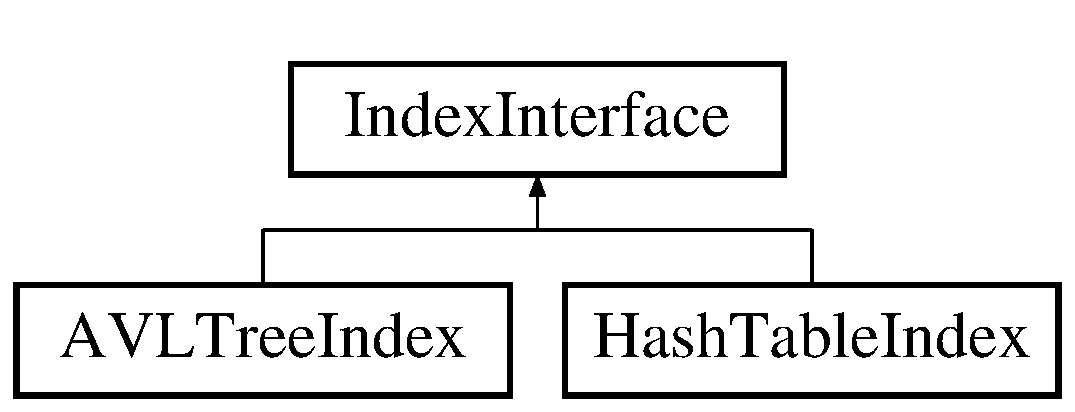
\includegraphics[height=2.000000cm]{class_index_interface}
\end{center}
\end{figure}
\subsection*{Public Member Functions}
\begin{DoxyCompactItemize}
\item 
\hyperlink{class_index_interface_a7b1e7eae7faa652d2f63efeecf0ca2de}{Index\+Interface} ()
\begin{DoxyCompactList}\small\item\em Initializes the member data with default values. \end{DoxyCompactList}\item 
virtual \hyperlink{class_index_interface_a3927fabe77a7da5845dc0495b2c1c2b2}{$\sim$\+Index\+Interface} ()
\begin{DoxyCompactList}\small\item\em Virtual destructor for proper memory management of this and child classes. \end{DoxyCompactList}\item 
virtual void \hyperlink{class_index_interface_aa7601d76e8cc3f0657e800efdc4c127e}{add\+Document} (const std\+::string \&path)=0
\begin{DoxyCompactList}\small\item\em Virtual function for adding a document. \end{DoxyCompactList}\item 
virtual void \hyperlink{class_index_interface_aac36b4561598ee84c0c68958a1e3f82b}{clear\+Index} ()=0
\begin{DoxyCompactList}\small\item\em Virtual function for clearing the index. \end{DoxyCompactList}\item 
virtual bool \hyperlink{class_index_interface_aaf90058a62e096bf607ea3dec2545ee4}{empty\+Index} () const  =0
\begin{DoxyCompactList}\small\item\em Virtual function for returning whether the index is empty. \end{DoxyCompactList}\item 
virtual \hyperlink{class_token}{Token} \hyperlink{class_index_interface_aa0ea18e7daa9984240d108bd765b2816}{find\+Word} (std\+::string \&term)=0
\begin{DoxyCompactList}\small\item\em Virtual function for finding a word in the index. \end{DoxyCompactList}\item 
virtual const \hyperlink{class_document}{Document} \& \hyperlink{class_index_interface_aa694a3e8feb722519b45f7313281bfad}{get\+Document\+By\+I\+D} (const int \&doc\+I\+D)=0
\begin{DoxyCompactList}\small\item\em Virtual function for getting a document pertaining to a given I\+D number. \end{DoxyCompactList}\item 
int \hyperlink{class_index_interface_af5d7e170720c26b3d38499d4e5e1dd69}{get\+Num\+Docs} () const 
\begin{DoxyCompactList}\small\item\em Returns the number of documents processed. \end{DoxyCompactList}\item 
int \hyperlink{class_index_interface_a3260a1213d90bd6cb6fd33043fb28b44}{get\+Num\+Tokens} () const 
\begin{DoxyCompactList}\small\item\em Returns the number of tokens processed. \end{DoxyCompactList}\item 
virtual bool \hyperlink{class_index_interface_a8ccd80a03123406cb4b1e2494349f9da}{has\+Word} (std\+::string \&term)=0
\begin{DoxyCompactList}\small\item\em Virtual function for returning whether the index contains a given word. \end{DoxyCompactList}\item 
virtual void \hyperlink{class_index_interface_ad8567919eafa87ac20c35928c929084d}{list\+Index} ()=0
\begin{DoxyCompactList}\small\item\em Virtual function for writing the persistent index. \end{DoxyCompactList}\item 
virtual bool \hyperlink{class_index_interface_a006f773f4e143745474e847cfb9f27fc}{load\+Index} ()=0
\begin{DoxyCompactList}\small\item\em Virtual function for loading an index in from persistent state. \end{DoxyCompactList}\item 
virtual bool \hyperlink{class_index_interface_a7b2ae510fa62eebb654708b90972c1b6}{make\+Index} (const std\+::string \&file\+Name)=0
\begin{DoxyCompactList}\small\item\em Virtual function for creating the index. \end{DoxyCompactList}\end{DoxyCompactItemize}


\subsection{Detailed Description}
Class for dealing with the index. 

\begin{DoxySeeAlso}{See also}
\hyperlink{class_a_v_l_tree_index}{A\+V\+L\+Tree\+Index}. 

\hyperlink{class_hash_table_index}{Hash\+Table\+Index}. 
\end{DoxySeeAlso}


\subsection{Constructor \& Destructor Documentation}
\hypertarget{class_index_interface_a7b1e7eae7faa652d2f63efeecf0ca2de}{}\index{Index\+Interface@{Index\+Interface}!Index\+Interface@{Index\+Interface}}
\index{Index\+Interface@{Index\+Interface}!Index\+Interface@{Index\+Interface}}
\subsubsection[{Index\+Interface()}]{\setlength{\rightskip}{0pt plus 5cm}Index\+Interface\+::\+Index\+Interface (
\begin{DoxyParamCaption}
{}
\end{DoxyParamCaption}
)\hspace{0.3cm}{\ttfamily [inline]}}\label{class_index_interface_a7b1e7eae7faa652d2f63efeecf0ca2de}


Initializes the member data with default values. 

\hypertarget{class_index_interface_a3927fabe77a7da5845dc0495b2c1c2b2}{}\index{Index\+Interface@{Index\+Interface}!````~Index\+Interface@{$\sim$\+Index\+Interface}}
\index{````~Index\+Interface@{$\sim$\+Index\+Interface}!Index\+Interface@{Index\+Interface}}
\subsubsection[{$\sim$\+Index\+Interface()}]{\setlength{\rightskip}{0pt plus 5cm}Index\+Interface\+::$\sim$\+Index\+Interface (
\begin{DoxyParamCaption}
{}
\end{DoxyParamCaption}
)\hspace{0.3cm}{\ttfamily [inline]}, {\ttfamily [virtual]}}\label{class_index_interface_a3927fabe77a7da5845dc0495b2c1c2b2}


Virtual destructor for proper memory management of this and child classes. 



\subsection{Member Function Documentation}
\hypertarget{class_index_interface_aa7601d76e8cc3f0657e800efdc4c127e}{}\index{Index\+Interface@{Index\+Interface}!add\+Document@{add\+Document}}
\index{add\+Document@{add\+Document}!Index\+Interface@{Index\+Interface}}
\subsubsection[{add\+Document(const std\+::string \&path)=0}]{\setlength{\rightskip}{0pt plus 5cm}Index\+Interface\+::add\+Document (
\begin{DoxyParamCaption}
\item[{const std\+::string \&}]{path}
\end{DoxyParamCaption}
)\hspace{0.3cm}{\ttfamily [pure virtual]}}\label{class_index_interface_aa7601d76e8cc3f0657e800efdc4c127e}


Virtual function for adding a document. 


\begin{DoxyParams}{Parameters}
{\em path} & -\/ a path to a file to add to the index. \\
\hline
\end{DoxyParams}


Implemented in \hyperlink{class_hash_table_index_a5387a8b9f0e585105a79624a93cd6ec0}{Hash\+Table\+Index}, and \hyperlink{class_a_v_l_tree_index_a1f84720f7580bd785a11d0e0425bd537}{A\+V\+L\+Tree\+Index}.

\hypertarget{class_index_interface_aac36b4561598ee84c0c68958a1e3f82b}{}\index{Index\+Interface@{Index\+Interface}!clear\+Index@{clear\+Index}}
\index{clear\+Index@{clear\+Index}!Index\+Interface@{Index\+Interface}}
\subsubsection[{clear\+Index()=0}]{\setlength{\rightskip}{0pt plus 5cm}Index\+Interface\+::clear\+Index (
\begin{DoxyParamCaption}
{}
\end{DoxyParamCaption}
)\hspace{0.3cm}{\ttfamily [pure virtual]}}\label{class_index_interface_aac36b4561598ee84c0c68958a1e3f82b}


Virtual function for clearing the index. 



Implemented in \hyperlink{class_hash_table_index_a69b31cc0bb54877b628bd67dadc5973f}{Hash\+Table\+Index}, and \hyperlink{class_a_v_l_tree_index_a1a877f264d30b657f37c6ed070d2e250}{A\+V\+L\+Tree\+Index}.

\hypertarget{class_index_interface_aaf90058a62e096bf607ea3dec2545ee4}{}\index{Index\+Interface@{Index\+Interface}!empty\+Index@{empty\+Index}}
\index{empty\+Index@{empty\+Index}!Index\+Interface@{Index\+Interface}}
\subsubsection[{empty\+Index() const  =0}]{\setlength{\rightskip}{0pt plus 5cm}Index\+Interface\+::empty\+Index (
\begin{DoxyParamCaption}
{}
\end{DoxyParamCaption}
) const\hspace{0.3cm}{\ttfamily [pure virtual]}}\label{class_index_interface_aaf90058a62e096bf607ea3dec2545ee4}


Virtual function for returning whether the index is empty. 

\begin{DoxyReturn}{Returns}
boolean whether the index is empty. 
\end{DoxyReturn}


Implemented in \hyperlink{class_hash_table_index_a19b62a531429e670b25cd92be4333890}{Hash\+Table\+Index}, and \hyperlink{class_a_v_l_tree_index_a447e5741c289869d5a5188def065fb6c}{A\+V\+L\+Tree\+Index}.

\hypertarget{class_index_interface_aa0ea18e7daa9984240d108bd765b2816}{}\index{Index\+Interface@{Index\+Interface}!find\+Word@{find\+Word}}
\index{find\+Word@{find\+Word}!Index\+Interface@{Index\+Interface}}
\subsubsection[{find\+Word(std\+::string \&term)=0}]{\setlength{\rightskip}{0pt plus 5cm}Index\+Interface\+::find\+Word (
\begin{DoxyParamCaption}
\item[{std\+::string \&}]{term}
\end{DoxyParamCaption}
)\hspace{0.3cm}{\ttfamily [pure virtual]}}\label{class_index_interface_aa0ea18e7daa9984240d108bd765b2816}


Virtual function for finding a word in the index. 


\begin{DoxyParams}{Parameters}
{\em term} & -\/ term to search for in the index. \\
\hline
\end{DoxyParams}
\begin{DoxyReturn}{Returns}
\hyperlink{class_token}{Token} (by value for \hyperlink{class_hash_table_index}{Hash\+Table\+Index} compatibility) representing the searched word. 
\end{DoxyReturn}


Implemented in \hyperlink{class_hash_table_index_a3d4c8e0244943cc44f33a35b742f7578}{Hash\+Table\+Index}, and \hyperlink{class_a_v_l_tree_index_ab549fb6b9fdf08926540f6652859d442}{A\+V\+L\+Tree\+Index}.

\hypertarget{class_index_interface_aa694a3e8feb722519b45f7313281bfad}{}\index{Index\+Interface@{Index\+Interface}!get\+Document\+By\+I\+D@{get\+Document\+By\+I\+D}}
\index{get\+Document\+By\+I\+D@{get\+Document\+By\+I\+D}!Index\+Interface@{Index\+Interface}}
\subsubsection[{get\+Document\+By\+I\+D(const int \&doc\+I\+D)=0}]{\setlength{\rightskip}{0pt plus 5cm}Index\+Interface\+::get\+Document\+By\+I\+D (
\begin{DoxyParamCaption}
\item[{const int \&}]{doc\+I\+D}
\end{DoxyParamCaption}
)\hspace{0.3cm}{\ttfamily [pure virtual]}}\label{class_index_interface_aa694a3e8feb722519b45f7313281bfad}


Virtual function for getting a document pertaining to a given I\+D number. 


\begin{DoxyParams}{Parameters}
{\em doc\+I\+D} & -\/ a document I\+D number. \\
\hline
\end{DoxyParams}
\begin{DoxyReturn}{Returns}
\hyperlink{class_document}{Document} reference. 
\end{DoxyReturn}


Implemented in \hyperlink{class_hash_table_index_ac5cc9451bce6e13739af7c5f154eea0b}{Hash\+Table\+Index}, and \hyperlink{class_a_v_l_tree_index_a0716178493a342dd6b790cfa8d01b3fa}{A\+V\+L\+Tree\+Index}.

\hypertarget{class_index_interface_af5d7e170720c26b3d38499d4e5e1dd69}{}\index{Index\+Interface@{Index\+Interface}!get\+Num\+Docs@{get\+Num\+Docs}}
\index{get\+Num\+Docs@{get\+Num\+Docs}!Index\+Interface@{Index\+Interface}}
\subsubsection[{get\+Num\+Docs() const }]{\setlength{\rightskip}{0pt plus 5cm}Index\+Interface\+::get\+Num\+Docs (
\begin{DoxyParamCaption}
{}
\end{DoxyParamCaption}
) const\hspace{0.3cm}{\ttfamily [inline]}}\label{class_index_interface_af5d7e170720c26b3d38499d4e5e1dd69}


Returns the number of documents processed. 

\begin{DoxyReturn}{Returns}
integer representing the number of documents processed. 
\end{DoxyReturn}
\hypertarget{class_index_interface_a3260a1213d90bd6cb6fd33043fb28b44}{}\index{Index\+Interface@{Index\+Interface}!get\+Num\+Tokens@{get\+Num\+Tokens}}
\index{get\+Num\+Tokens@{get\+Num\+Tokens}!Index\+Interface@{Index\+Interface}}
\subsubsection[{get\+Num\+Tokens() const }]{\setlength{\rightskip}{0pt plus 5cm}Index\+Interface\+::get\+Num\+Tokens (
\begin{DoxyParamCaption}
{}
\end{DoxyParamCaption}
) const\hspace{0.3cm}{\ttfamily [inline]}}\label{class_index_interface_a3260a1213d90bd6cb6fd33043fb28b44}


Returns the number of tokens processed. 

\begin{DoxyReturn}{Returns}
integer representing the number of tokens processed. 
\end{DoxyReturn}
\hypertarget{class_index_interface_a8ccd80a03123406cb4b1e2494349f9da}{}\index{Index\+Interface@{Index\+Interface}!has\+Word@{has\+Word}}
\index{has\+Word@{has\+Word}!Index\+Interface@{Index\+Interface}}
\subsubsection[{has\+Word(std\+::string \&term)=0}]{\setlength{\rightskip}{0pt plus 5cm}Index\+Interface\+::has\+Word (
\begin{DoxyParamCaption}
\item[{std\+::string \&}]{term}
\end{DoxyParamCaption}
)\hspace{0.3cm}{\ttfamily [pure virtual]}}\label{class_index_interface_a8ccd80a03123406cb4b1e2494349f9da}


Virtual function for returning whether the index contains a given word. 


\begin{DoxyParams}{Parameters}
{\em term} & -\/ a term to search the index for. \\
\hline
\end{DoxyParams}
\begin{DoxyReturn}{Returns}
boolean whether the index contains the word. 
\end{DoxyReturn}


Implemented in \hyperlink{class_hash_table_index_aea9366ff9299d41bd3447bc6c95a3960}{Hash\+Table\+Index}, and \hyperlink{class_a_v_l_tree_index_acb31068c39161358ec6545df5feaabc0}{A\+V\+L\+Tree\+Index}.

\hypertarget{class_index_interface_ad8567919eafa87ac20c35928c929084d}{}\index{Index\+Interface@{Index\+Interface}!list\+Index@{list\+Index}}
\index{list\+Index@{list\+Index}!Index\+Interface@{Index\+Interface}}
\subsubsection[{list\+Index()=0}]{\setlength{\rightskip}{0pt plus 5cm}Index\+Interface\+::list\+Index (
\begin{DoxyParamCaption}
{}
\end{DoxyParamCaption}
)\hspace{0.3cm}{\ttfamily [pure virtual]}}\label{class_index_interface_ad8567919eafa87ac20c35928c929084d}


Virtual function for writing the persistent index. 



Implemented in \hyperlink{class_hash_table_index_a42bbd9b325fb95b54a546c3c98c67624}{Hash\+Table\+Index}, and \hyperlink{class_a_v_l_tree_index_a603741ace3489018f33f5ba4282e3f0d}{A\+V\+L\+Tree\+Index}.

\hypertarget{class_index_interface_a006f773f4e143745474e847cfb9f27fc}{}\index{Index\+Interface@{Index\+Interface}!load\+Index@{load\+Index}}
\index{load\+Index@{load\+Index}!Index\+Interface@{Index\+Interface}}
\subsubsection[{load\+Index()=0}]{\setlength{\rightskip}{0pt plus 5cm}Index\+Interface\+::load\+Index (
\begin{DoxyParamCaption}
{}
\end{DoxyParamCaption}
)\hspace{0.3cm}{\ttfamily [pure virtual]}}\label{class_index_interface_a006f773f4e143745474e847cfb9f27fc}


Virtual function for loading an index in from persistent state. 

\begin{DoxyReturn}{Returns}
boolean whether the index was successfully loaded. 
\end{DoxyReturn}


Implemented in \hyperlink{class_hash_table_index_a8c483a83b40b49b0f35be9fea0674501}{Hash\+Table\+Index}, and \hyperlink{class_a_v_l_tree_index_af161b8697db7e3f599abc78a36f8d145}{A\+V\+L\+Tree\+Index}.

\hypertarget{class_index_interface_a7b2ae510fa62eebb654708b90972c1b6}{}\index{Index\+Interface@{Index\+Interface}!make\+Index@{make\+Index}}
\index{make\+Index@{make\+Index}!Index\+Interface@{Index\+Interface}}
\subsubsection[{make\+Index(const std\+::string \&file\+Name)=0}]{\setlength{\rightskip}{0pt plus 5cm}Index\+Interface\+::make\+Index (
\begin{DoxyParamCaption}
\item[{const std\+::string \&}]{file\+Name}
\end{DoxyParamCaption}
)\hspace{0.3cm}{\ttfamily [pure virtual]}}\label{class_index_interface_a7b2ae510fa62eebb654708b90972c1b6}


Virtual function for creating the index. 


\begin{DoxyParams}{Parameters}
{\em file\+Name} & -\/ a directory containing files to be put in the index. \\
\hline
\end{DoxyParams}
\begin{DoxyReturn}{Returns}
boolean whether the index was successfully created. 
\end{DoxyReturn}


Implemented in \hyperlink{class_hash_table_index_a5105f715d8c5fd3b74d6bec462cb0c38}{Hash\+Table\+Index}, and \hyperlink{class_a_v_l_tree_index_a37200f167e48a7b24cb012b9ff5cf44c}{A\+V\+L\+Tree\+Index}.



The documentation for this class was generated from the following file\+:\begin{DoxyCompactItemize}
\item 
\hyperlink{_index_interface_8hpp}{Index\+Interface.\+hpp}\end{DoxyCompactItemize}

\hypertarget{structnode}{}\section{node$<$ \+\_\+\+Type $>$ Struct Template Reference}
\label{structnode}\index{node$<$ \+\_\+\+Type $>$@{node$<$ \+\_\+\+Type $>$}}


A node for use in the A\+V\+L tree. Holds a value, height, and pointers to left and right child nodes.  




{\ttfamily \#include $<$A\+V\+L\+Tree.\+hpp$>$}

\subsection*{Public Member Functions}
\begin{DoxyCompactItemize}
\item 
\hyperlink{structnode_a07f56d66b295e3a51cd8e5771c505e2f}{node} ()
\begin{DoxyCompactList}\small\item\em Initializes the member data with default values. \end{DoxyCompactList}\item 
\hyperlink{structnode_a57d8701648d6e65867648f077add339b}{node} (const \hyperlink{structnode}{node} \&copy)
\begin{DoxyCompactList}\small\item\em Copy constructor. \end{DoxyCompactList}\item 
\hyperlink{structnode_ac422b5fa2f7dc1bfc6485373f4a37cf8}{node} (\hyperlink{structnode}{node} \&\&copy)
\begin{DoxyCompactList}\small\item\em Move constructor. \end{DoxyCompactList}\item 
\hyperlink{structnode_a48762381e551e35cb9ee0d515339dab0}{node} (const value\+\_\+type \&value, \hyperlink{structnode}{node} $\ast$parent, \hyperlink{structnode}{node} $\ast$left, \hyperlink{structnode}{node} $\ast$right)
\begin{DoxyCompactList}\small\item\em Initializes the member data with a given value and pointers to a parent, left, and right child and a height of -\/1. \end{DoxyCompactList}\item 
\hyperlink{structnode_a7eb8c2ea4c2dfeb90bef1ecee16aa0f9}{node} (const value\+\_\+type \&value, const int \&height, \hyperlink{structnode}{node} $\ast$parent, \hyperlink{structnode}{node} $\ast$left, \hyperlink{structnode}{node} $\ast$right)
\item 
\hyperlink{structnode_a527872acc0945cc69fdcc1237112ea40}{$\sim$node} ()
\begin{DoxyCompactList}\small\item\em Destructor. \end{DoxyCompactList}\item 
\hyperlink{structnode}{node} \& \hyperlink{structnode_a88b75549d8936a1cdafd77d1daf9f218}{operator=} (\hyperlink{structnode}{node} copy)
\begin{DoxyCompactList}\small\item\em Assignment operator; uses copy-\/swap idiom. \end{DoxyCompactList}\end{DoxyCompactItemize}
\subsection*{Public Attributes}
\begin{DoxyCompactItemize}
\item 
value\+\_\+type \hyperlink{structnode_a8353cf23af61f2a637764a1a46ca8eb6}{\+\_\+value}
\begin{DoxyCompactList}\small\item\em Value stored in the node. \end{DoxyCompactList}\item 
int \hyperlink{structnode_a3acd2c366e647bce759f961f71ebf5b3}{\+\_\+height}
\begin{DoxyCompactList}\small\item\em Height of the node in the tree. \end{DoxyCompactList}\item 
\hyperlink{structnode}{node} $\ast$ \hyperlink{structnode_ad045681eca718a3867a16a9644aac2a6}{\+\_\+parent}
\begin{DoxyCompactList}\small\item\em A pointer to the parent of the node. \end{DoxyCompactList}\item 
\hyperlink{structnode}{node} $\ast$ \hyperlink{structnode_af082014da104d7b72a3b7299d027ffbb}{\+\_\+left}
\begin{DoxyCompactList}\small\item\em A pointer to the left child of the node. \end{DoxyCompactList}\item 
\hyperlink{structnode}{node} $\ast$ \hyperlink{structnode_aa65c4746c7391fb99f06fec3400addce}{\+\_\+right}
\begin{DoxyCompactList}\small\item\em A pointer to the right child of the node. \end{DoxyCompactList}\end{DoxyCompactItemize}
\subsection*{Friends}
\begin{DoxyCompactItemize}
\item 
{\footnotesize template$<$class \+\_\+\+Type1 $>$ }\\void \hyperlink{structnode_ae91b864585481f95d662fe66839e3e42}{swap} (\hyperlink{structnode}{node}$<$ \+\_\+\+Type $>$ \&lhs, \hyperlink{structnode}{node}$<$ \+\_\+\+Type $>$ \&rhs)
\begin{DoxyCompactList}\small\item\em friend swap function for external use. \end{DoxyCompactList}\end{DoxyCompactItemize}


\subsection{Detailed Description}
\subsubsection*{template$<$class \+\_\+\+Type$>$struct node$<$ \+\_\+\+Type $>$}

A node for use in the A\+V\+L tree. Holds a value, height, and pointers to left and right child nodes. 


\begin{DoxyParams}{Parameters}
{\em \+\_\+\+Type} & -\/ a type for the node template. \\
\hline
\end{DoxyParams}
\begin{DoxySeeAlso}{See also}
\hyperlink{class_a_v_l_tree}{A\+V\+L\+Tree}. 
\end{DoxySeeAlso}


\subsection{Constructor \& Destructor Documentation}
\hypertarget{structnode_a07f56d66b295e3a51cd8e5771c505e2f}{}\index{node@{node}!node@{node}}
\index{node@{node}!node@{node}}
\subsubsection[{node()}]{\setlength{\rightskip}{0pt plus 5cm}template$<$class \+\_\+\+Type$>$ {\bf node}$<$ \+\_\+\+Type $>$\+::{\bf node} (
\begin{DoxyParamCaption}
{}
\end{DoxyParamCaption}
)\hspace{0.3cm}{\ttfamily [inline]}}\label{structnode_a07f56d66b295e3a51cd8e5771c505e2f}


Initializes the member data with default values. 

\hypertarget{structnode_a57d8701648d6e65867648f077add339b}{}\index{node@{node}!node@{node}}
\index{node@{node}!node@{node}}
\subsubsection[{node(const node \&copy)}]{\setlength{\rightskip}{0pt plus 5cm}template$<$class \+\_\+\+Type$>$ {\bf node}$<$ \+\_\+\+Type $>$\+::{\bf node} (
\begin{DoxyParamCaption}
\item[{const {\bf node}$<$ \+\_\+\+Type $>$ \&}]{copy}
\end{DoxyParamCaption}
)\hspace{0.3cm}{\ttfamily [inline]}}\label{structnode_a57d8701648d6e65867648f077add339b}


Copy constructor. 


\begin{DoxyParams}{Parameters}
{\em copy} & -\/ another node to copy. \\
\hline
\end{DoxyParams}
\hypertarget{structnode_ac422b5fa2f7dc1bfc6485373f4a37cf8}{}\index{node@{node}!node@{node}}
\index{node@{node}!node@{node}}
\subsubsection[{node(node \&\&copy)}]{\setlength{\rightskip}{0pt plus 5cm}template$<$class \+\_\+\+Type$>$ {\bf node}$<$ \+\_\+\+Type $>$\+::{\bf node} (
\begin{DoxyParamCaption}
\item[{{\bf node}$<$ \+\_\+\+Type $>$ \&\&}]{copy}
\end{DoxyParamCaption}
)\hspace{0.3cm}{\ttfamily [inline]}}\label{structnode_ac422b5fa2f7dc1bfc6485373f4a37cf8}


Move constructor. 


\begin{DoxyParams}{Parameters}
{\em copy} & -\/ another node to move from. \\
\hline
\end{DoxyParams}
\hypertarget{structnode_a48762381e551e35cb9ee0d515339dab0}{}\index{node@{node}!node@{node}}
\index{node@{node}!node@{node}}
\subsubsection[{node(const value\+\_\+type \&value, node $\ast$parent, node $\ast$left, node $\ast$right)}]{\setlength{\rightskip}{0pt plus 5cm}template$<$class \+\_\+\+Type$>$ {\bf node}$<$ \+\_\+\+Type $>$\+::{\bf node} (
\begin{DoxyParamCaption}
\item[{const value\+\_\+type \&}]{value, }
\item[{{\bf node}$<$ \+\_\+\+Type $>$ $\ast$}]{parent, }
\item[{{\bf node}$<$ \+\_\+\+Type $>$ $\ast$}]{left, }
\item[{{\bf node}$<$ \+\_\+\+Type $>$ $\ast$}]{right}
\end{DoxyParamCaption}
)\hspace{0.3cm}{\ttfamily [inline]}}\label{structnode_a48762381e551e35cb9ee0d515339dab0}


Initializes the member data with a given value and pointers to a parent, left, and right child and a height of -\/1. 


\begin{DoxyParams}{Parameters}
{\em value} & -\/ a value of type value\+\_\+type. \\
\hline
{\em parent} & -\/ a pointer to the parent of the new node (should almost always be nullptr). \\
\hline
{\em left} & -\/ a pointer to the left child of the new node (should almost always be nullptr). \\
\hline
{\em right} & -\/ a pointer to the right child of the new node (should almost always be nullptr). \\
\hline
\end{DoxyParams}
\hypertarget{structnode_a7eb8c2ea4c2dfeb90bef1ecee16aa0f9}{}\index{node@{node}!node@{node}}
\index{node@{node}!node@{node}}
\subsubsection[{node(const value\+\_\+type \&value, const int \&height, node $\ast$parent, node $\ast$left, node $\ast$right)}]{\setlength{\rightskip}{0pt plus 5cm}template$<$class \+\_\+\+Type$>$ {\bf node}$<$ \+\_\+\+Type $>$\+::{\bf node} (
\begin{DoxyParamCaption}
\item[{const value\+\_\+type \&}]{value, }
\item[{const int \&}]{height, }
\item[{{\bf node}$<$ \+\_\+\+Type $>$ $\ast$}]{parent, }
\item[{{\bf node}$<$ \+\_\+\+Type $>$ $\ast$}]{left, }
\item[{{\bf node}$<$ \+\_\+\+Type $>$ $\ast$}]{right}
\end{DoxyParamCaption}
)\hspace{0.3cm}{\ttfamily [inline]}}\label{structnode_a7eb8c2ea4c2dfeb90bef1ecee16aa0f9}
\hypertarget{structnode_a527872acc0945cc69fdcc1237112ea40}{}\index{node@{node}!````~node@{$\sim$node}}
\index{````~node@{$\sim$node}!node@{node}}
\subsubsection[{$\sim$node()}]{\setlength{\rightskip}{0pt plus 5cm}template$<$class \+\_\+\+Type$>$ {\bf node}$<$ \+\_\+\+Type $>$\+::$\sim${\bf node} (
\begin{DoxyParamCaption}
{}
\end{DoxyParamCaption}
)\hspace{0.3cm}{\ttfamily [inline]}}\label{structnode_a527872acc0945cc69fdcc1237112ea40}


Destructor. 



\subsection{Member Function Documentation}
\hypertarget{structnode_a88b75549d8936a1cdafd77d1daf9f218}{}\index{node@{node}!operator=@{operator=}}
\index{operator=@{operator=}!node@{node}}
\subsubsection[{operator=(node copy)}]{\setlength{\rightskip}{0pt plus 5cm}template$<$class \+\_\+\+Type$>$ {\bf node}$<$ \+\_\+\+Type $>$\+::operator= (
\begin{DoxyParamCaption}
\item[{{\bf node}$<$ \+\_\+\+Type $>$}]{copy}
\end{DoxyParamCaption}
)\hspace{0.3cm}{\ttfamily [inline]}}\label{structnode_a88b75549d8936a1cdafd77d1daf9f218}


Assignment operator; uses copy-\/swap idiom. 


\begin{DoxyParams}{Parameters}
{\em copy} & -\/ a node passed by value. \\
\hline
\end{DoxyParams}
\begin{DoxyReturn}{Returns}
a reference to a node. 
\end{DoxyReturn}


\subsection{Friends And Related Function Documentation}
\hypertarget{structnode_ae91b864585481f95d662fe66839e3e42}{}\index{node@{node}!swap@{swap}}
\index{swap@{swap}!node@{node}}
\subsubsection[{swap}]{\setlength{\rightskip}{0pt plus 5cm}template$<$class \+\_\+\+Type$>$ template$<$class \+\_\+\+Type1 $>$ {\bf node}$<$ \+\_\+\+Type $>$\+::swap (
\begin{DoxyParamCaption}
\item[{{\bf node}$<$ \+\_\+\+Type $>$ \&}]{lhs, }
\item[{{\bf node}$<$ \+\_\+\+Type $>$ \&}]{rhs}
\end{DoxyParamCaption}
)\hspace{0.3cm}{\ttfamily [friend]}}\label{structnode_ae91b864585481f95d662fe66839e3e42}


friend swap function for external use. 


\begin{DoxyParams}{Parameters}
{\em lhs} & -\/ first node to be swapped. \\
\hline
{\em rhs} & -\/ second node to be swapped. \\
\hline
\end{DoxyParams}


\subsection{Member Data Documentation}
\hypertarget{structnode_a3acd2c366e647bce759f961f71ebf5b3}{}\index{node@{node}!\+\_\+height@{\+\_\+height}}
\index{\+\_\+height@{\+\_\+height}!node@{node}}
\subsubsection[{\+\_\+height}]{\setlength{\rightskip}{0pt plus 5cm}template$<$class \+\_\+\+Type$>$ int {\bf node}$<$ \+\_\+\+Type $>$\+::\+\_\+height}\label{structnode_a3acd2c366e647bce759f961f71ebf5b3}


Height of the node in the tree. 

\hypertarget{structnode_af082014da104d7b72a3b7299d027ffbb}{}\index{node@{node}!\+\_\+left@{\+\_\+left}}
\index{\+\_\+left@{\+\_\+left}!node@{node}}
\subsubsection[{\+\_\+left}]{\setlength{\rightskip}{0pt plus 5cm}template$<$class \+\_\+\+Type$>$ {\bf node}$\ast$ {\bf node}$<$ \+\_\+\+Type $>$\+::\+\_\+left}\label{structnode_af082014da104d7b72a3b7299d027ffbb}


A pointer to the left child of the node. 

\hypertarget{structnode_ad045681eca718a3867a16a9644aac2a6}{}\index{node@{node}!\+\_\+parent@{\+\_\+parent}}
\index{\+\_\+parent@{\+\_\+parent}!node@{node}}
\subsubsection[{\+\_\+parent}]{\setlength{\rightskip}{0pt plus 5cm}template$<$class \+\_\+\+Type$>$ {\bf node}$\ast$ {\bf node}$<$ \+\_\+\+Type $>$\+::\+\_\+parent}\label{structnode_ad045681eca718a3867a16a9644aac2a6}


A pointer to the parent of the node. 

\hypertarget{structnode_aa65c4746c7391fb99f06fec3400addce}{}\index{node@{node}!\+\_\+right@{\+\_\+right}}
\index{\+\_\+right@{\+\_\+right}!node@{node}}
\subsubsection[{\+\_\+right}]{\setlength{\rightskip}{0pt plus 5cm}template$<$class \+\_\+\+Type$>$ {\bf node}$\ast$ {\bf node}$<$ \+\_\+\+Type $>$\+::\+\_\+right}\label{structnode_aa65c4746c7391fb99f06fec3400addce}


A pointer to the right child of the node. 

\hypertarget{structnode_a8353cf23af61f2a637764a1a46ca8eb6}{}\index{node@{node}!\+\_\+value@{\+\_\+value}}
\index{\+\_\+value@{\+\_\+value}!node@{node}}
\subsubsection[{\+\_\+value}]{\setlength{\rightskip}{0pt plus 5cm}template$<$class \+\_\+\+Type$>$ value\+\_\+type {\bf node}$<$ \+\_\+\+Type $>$\+::\+\_\+value}\label{structnode_a8353cf23af61f2a637764a1a46ca8eb6}


Value stored in the node. 



The documentation for this struct was generated from the following file\+:\begin{DoxyCompactItemize}
\item 
\hyperlink{_a_v_l_tree_8hpp}{A\+V\+L\+Tree.\+hpp}\end{DoxyCompactItemize}

\hypertarget{class_query_processor}{}\section{Query\+Processor Class Reference}
\label{class_query_processor}\index{Query\+Processor@{Query\+Processor}}


Class for parsing user queries and ranking results.  




{\ttfamily \#include $<$Query\+Processor.\+hpp$>$}

\subsection*{Public Member Functions}
\begin{DoxyCompactItemize}
\item 
\hyperlink{class_query_processor_a32a6760ff0aab51b38fb8eb236e2e140}{Query\+Processor} ()
\begin{DoxyCompactList}\small\item\em Initializes the member data with default values. \end{DoxyCompactList}\item 
set\+\_\+type \hyperlink{class_query_processor_a24544d09490d3ef704acaae4f3d5d478}{process\+Terms} (std\+::vector$<$ std\+::string $>$ \&terms, \hyperlink{class_index_interface}{Index\+Interface} \&indexer)
\begin{DoxyCompactList}\small\item\em parses the query based on boolean terms if any and returns a set of results if any. \end{DoxyCompactList}\item 
void \hyperlink{class_query_processor_a08d7a42132998959c37e75ec61d5662c}{search} (std\+::string \&query, \hyperlink{class_index_interface}{Index\+Interface} \&indexer)
\begin{DoxyCompactList}\small\item\em Performs a search based on the given query; sends the tokenized query to \hyperlink{class_query_processor_a24544d09490d3ef704acaae4f3d5d478}{process\+Terms()}; also outputs the results. \end{DoxyCompactList}\item 
void \hyperlink{class_query_processor_a9bf3ee98ae9154d55ea70051ea199673}{set\+Num\+Docs} (const \hyperlink{class_index_interface}{Index\+Interface} \&indexer)
\begin{DoxyCompactList}\small\item\em Sets the number of documents processed; for use in calculating tf-\/idf values. \end{DoxyCompactList}\end{DoxyCompactItemize}


\subsection{Detailed Description}
Class for parsing user queries and ranking results. 

\begin{DoxySeeAlso}{See also}
\hyperlink{class_index_interface}{Index\+Interface}. 
\end{DoxySeeAlso}


\subsection{Constructor \& Destructor Documentation}
\hypertarget{class_query_processor_a32a6760ff0aab51b38fb8eb236e2e140}{}\index{Query\+Processor@{Query\+Processor}!Query\+Processor@{Query\+Processor}}
\index{Query\+Processor@{Query\+Processor}!Query\+Processor@{Query\+Processor}}
\subsubsection[{Query\+Processor()}]{\setlength{\rightskip}{0pt plus 5cm}Query\+Processor\+::\+Query\+Processor (
\begin{DoxyParamCaption}
{}
\end{DoxyParamCaption}
)}\label{class_query_processor_a32a6760ff0aab51b38fb8eb236e2e140}


Initializes the member data with default values. 



\subsection{Member Function Documentation}
\hypertarget{class_query_processor_a24544d09490d3ef704acaae4f3d5d478}{}\index{Query\+Processor@{Query\+Processor}!process\+Terms@{process\+Terms}}
\index{process\+Terms@{process\+Terms}!Query\+Processor@{Query\+Processor}}
\subsubsection[{process\+Terms(std\+::vector$<$ std\+::string $>$ \&terms, Index\+Interface \&indexer)}]{\setlength{\rightskip}{0pt plus 5cm}Query\+Processor\+::process\+Terms (
\begin{DoxyParamCaption}
\item[{std\+::vector$<$ std\+::string $>$ \&}]{terms, }
\item[{{\bf Index\+Interface} \&}]{indexer}
\end{DoxyParamCaption}
)}\label{class_query_processor_a24544d09490d3ef704acaae4f3d5d478}


parses the query based on boolean terms if any and returns a set of results if any. 


\begin{DoxyParams}{Parameters}
{\em terms} & -\/ a std\+::vector containing the search terms to be processed. \\
\hline
{\em indexer} & -\/ an indexing object; one of either \hyperlink{class_a_v_l_tree_index}{A\+V\+L\+Tree\+Index} or \hyperlink{class_hash_table_index}{Hash\+Table\+Index}. \\
\hline
\end{DoxyParams}
\begin{DoxyReturn}{Returns}
a set\+\_\+type containing the search results. 
\end{DoxyReturn}
\hypertarget{class_query_processor_a08d7a42132998959c37e75ec61d5662c}{}\index{Query\+Processor@{Query\+Processor}!search@{search}}
\index{search@{search}!Query\+Processor@{Query\+Processor}}
\subsubsection[{search(std\+::string \&query, Index\+Interface \&indexer)}]{\setlength{\rightskip}{0pt plus 5cm}Query\+Processor\+::search (
\begin{DoxyParamCaption}
\item[{std\+::string \&}]{query, }
\item[{{\bf Index\+Interface} \&}]{indexer}
\end{DoxyParamCaption}
)}\label{class_query_processor_a08d7a42132998959c37e75ec61d5662c}


Performs a search based on the given query; sends the tokenized query to \hyperlink{class_query_processor_a24544d09490d3ef704acaae4f3d5d478}{process\+Terms()}; also outputs the results. 


\begin{DoxyParams}{Parameters}
{\em query} & -\/ a string to search the index for. \\
\hline
{\em indexer} & -\/ an indexing object; one of either \hyperlink{class_a_v_l_tree_index}{A\+V\+L\+Tree\+Index} or \hyperlink{class_hash_table_index}{Hash\+Table\+Index}. \\
\hline
\end{DoxyParams}
\hypertarget{class_query_processor_a9bf3ee98ae9154d55ea70051ea199673}{}\index{Query\+Processor@{Query\+Processor}!set\+Num\+Docs@{set\+Num\+Docs}}
\index{set\+Num\+Docs@{set\+Num\+Docs}!Query\+Processor@{Query\+Processor}}
\subsubsection[{set\+Num\+Docs(const Index\+Interface \&indexer)}]{\setlength{\rightskip}{0pt plus 5cm}Query\+Processor\+::set\+Num\+Docs (
\begin{DoxyParamCaption}
\item[{const {\bf Index\+Interface} \&}]{indexer}
\end{DoxyParamCaption}
)\hspace{0.3cm}{\ttfamily [inline]}}\label{class_query_processor_a9bf3ee98ae9154d55ea70051ea199673}


Sets the number of documents processed; for use in calculating tf-\/idf values. 


\begin{DoxyParams}{Parameters}
{\em indexer} & -\/ an indexing object; one of either \hyperlink{class_a_v_l_tree_index}{A\+V\+L\+Tree\+Index} or \hyperlink{class_hash_table_index}{Hash\+Table\+Index}. \\
\hline
\end{DoxyParams}


The documentation for this class was generated from the following files\+:\begin{DoxyCompactItemize}
\item 
\hyperlink{_query_processor_8hpp}{Query\+Processor.\+hpp}\item 
\hyperlink{_query_processor_8cpp}{Query\+Processor.\+cpp}\end{DoxyCompactItemize}

\hypertarget{class_search_engine}{}\section{Search\+Engine Class Reference}
\label{class_search_engine}\index{Search\+Engine@{Search\+Engine}}


Class for performing U\+I functionality.  




{\ttfamily \#include $<$Search\+Engine.\+hpp$>$}

\subsection*{Public Member Functions}
\begin{DoxyCompactItemize}
\item 
\hyperlink{class_search_engine_ab129d2c96c29c6dcf4a28abbe4168f6c}{Search\+Engine} ()
\begin{DoxyCompactList}\small\item\em Initializes the member data with default values and loads in the last created index file. \end{DoxyCompactList}\item 
\hyperlink{class_search_engine_a863ab87efd742b9a8f20b87774ab570f}{$\sim$\+Search\+Engine} ()
\begin{DoxyCompactList}\small\item\em Deletes the pointer to the indexer if it has been initialized. \end{DoxyCompactList}\item 
void \hyperlink{class_search_engine_a9ea46878a950ecad2f9f4af265ab3ace}{add\+Document} (const std\+::string \&path)
\begin{DoxyCompactList}\small\item\em Adds a new document to the index. \end{DoxyCompactList}\item 
void \hyperlink{class_search_engine_a5418e11e3626e8a72d697346051c44fd}{clear\+Index} ()
\begin{DoxyCompactList}\small\item\em Clears the index. \end{DoxyCompactList}\item 
void \hyperlink{class_search_engine_a76393f870a6ce5591b140b81df9c5fac}{interactive} ()
\begin{DoxyCompactList}\small\item\em Displays the interactive menu. \end{DoxyCompactList}\item 
void \hyperlink{class_search_engine_ac492e86eaba0b6c7c270ee88e2d6d0ab}{launch\+U\+I} ()
\begin{DoxyCompactList}\small\item\em Displays the main menu. \end{DoxyCompactList}\item 
void \hyperlink{class_search_engine_ad269ece849be36f3be5b315e0a32a120}{maintenance} ()
\end{DoxyCompactItemize}


\subsection{Detailed Description}
Class for performing U\+I functionality. 

\begin{DoxySeeAlso}{See also}
\hyperlink{class_index_interface}{Index\+Interface}. 

\hyperlink{class_query_processor}{Query\+Processor}. 
\end{DoxySeeAlso}


\subsection{Constructor \& Destructor Documentation}
\hypertarget{class_search_engine_ab129d2c96c29c6dcf4a28abbe4168f6c}{}\index{Search\+Engine@{Search\+Engine}!Search\+Engine@{Search\+Engine}}
\index{Search\+Engine@{Search\+Engine}!Search\+Engine@{Search\+Engine}}
\subsubsection[{Search\+Engine()}]{\setlength{\rightskip}{0pt plus 5cm}Search\+Engine\+::\+Search\+Engine (
\begin{DoxyParamCaption}
{}
\end{DoxyParamCaption}
)}\label{class_search_engine_ab129d2c96c29c6dcf4a28abbe4168f6c}


Initializes the member data with default values and loads in the last created index file. 

\hypertarget{class_search_engine_a863ab87efd742b9a8f20b87774ab570f}{}\index{Search\+Engine@{Search\+Engine}!````~Search\+Engine@{$\sim$\+Search\+Engine}}
\index{````~Search\+Engine@{$\sim$\+Search\+Engine}!Search\+Engine@{Search\+Engine}}
\subsubsection[{$\sim$\+Search\+Engine()}]{\setlength{\rightskip}{0pt plus 5cm}Search\+Engine\+::$\sim$\+Search\+Engine (
\begin{DoxyParamCaption}
{}
\end{DoxyParamCaption}
)}\label{class_search_engine_a863ab87efd742b9a8f20b87774ab570f}


Deletes the pointer to the indexer if it has been initialized. 



\subsection{Member Function Documentation}
\hypertarget{class_search_engine_a9ea46878a950ecad2f9f4af265ab3ace}{}\index{Search\+Engine@{Search\+Engine}!add\+Document@{add\+Document}}
\index{add\+Document@{add\+Document}!Search\+Engine@{Search\+Engine}}
\subsubsection[{add\+Document(const std\+::string \&path)}]{\setlength{\rightskip}{0pt plus 5cm}Search\+Engine\+::add\+Document (
\begin{DoxyParamCaption}
\item[{const std\+::string \&}]{path}
\end{DoxyParamCaption}
)}\label{class_search_engine_a9ea46878a950ecad2f9f4af265ab3ace}


Adds a new document to the index. 


\begin{DoxyParams}{Parameters}
{\em path} & -\/ path to a file containing properly formatted X\+M\+L to parse. \\
\hline
\end{DoxyParams}
\hypertarget{class_search_engine_a5418e11e3626e8a72d697346051c44fd}{}\index{Search\+Engine@{Search\+Engine}!clear\+Index@{clear\+Index}}
\index{clear\+Index@{clear\+Index}!Search\+Engine@{Search\+Engine}}
\subsubsection[{clear\+Index()}]{\setlength{\rightskip}{0pt plus 5cm}Search\+Engine\+::clear\+Index (
\begin{DoxyParamCaption}
{}
\end{DoxyParamCaption}
)}\label{class_search_engine_a5418e11e3626e8a72d697346051c44fd}


Clears the index. 

\hypertarget{class_search_engine_a76393f870a6ce5591b140b81df9c5fac}{}\index{Search\+Engine@{Search\+Engine}!interactive@{interactive}}
\index{interactive@{interactive}!Search\+Engine@{Search\+Engine}}
\subsubsection[{interactive()}]{\setlength{\rightskip}{0pt plus 5cm}Search\+Engine\+::interactive (
\begin{DoxyParamCaption}
{}
\end{DoxyParamCaption}
)}\label{class_search_engine_a76393f870a6ce5591b140b81df9c5fac}


Displays the interactive menu. 

Displays the maintenance menu. \hypertarget{class_search_engine_ac492e86eaba0b6c7c270ee88e2d6d0ab}{}\index{Search\+Engine@{Search\+Engine}!launch\+U\+I@{launch\+U\+I}}
\index{launch\+U\+I@{launch\+U\+I}!Search\+Engine@{Search\+Engine}}
\subsubsection[{launch\+U\+I()}]{\setlength{\rightskip}{0pt plus 5cm}Search\+Engine\+::launch\+U\+I (
\begin{DoxyParamCaption}
{}
\end{DoxyParamCaption}
)}\label{class_search_engine_ac492e86eaba0b6c7c270ee88e2d6d0ab}


Displays the main menu. 

\hypertarget{class_search_engine_ad269ece849be36f3be5b315e0a32a120}{}\index{Search\+Engine@{Search\+Engine}!maintenance@{maintenance}}
\index{maintenance@{maintenance}!Search\+Engine@{Search\+Engine}}
\subsubsection[{maintenance()}]{\setlength{\rightskip}{0pt plus 5cm}void Search\+Engine\+::maintenance (
\begin{DoxyParamCaption}
{}
\end{DoxyParamCaption}
)}\label{class_search_engine_ad269ece849be36f3be5b315e0a32a120}


The documentation for this class was generated from the following files\+:\begin{DoxyCompactItemize}
\item 
\hyperlink{_search_engine_8hpp}{Search\+Engine.\+hpp}\item 
\hyperlink{_search_engine_8cpp}{Search\+Engine.\+cpp}\end{DoxyCompactItemize}

\hypertarget{class_token}{}\section{Token Class Reference}
\label{class_token}\index{Token@{Token}}


Class for representing each token in the corpus.  




{\ttfamily \#include $<$Token.\+hpp$>$}

\subsection*{Public Member Functions}
\begin{DoxyCompactItemize}
\item 
\hyperlink{class_token_aa3c5868ba4115f3189df6b2ac5b36f39}{Token} ()
\begin{DoxyCompactList}\small\item\em Initializes the member data with default values. \end{DoxyCompactList}\item 
\hyperlink{class_token_afbdab46261b6980bebf75e1c910d19ec}{Token} (const std\+::string \&\hyperlink{class_token_a518dac411db3279a9b2f4ce38e46d199}{payload})
\begin{DoxyCompactList}\small\item\em Initializes the member data with a given payload and default values for the rest of the data members. \end{DoxyCompactList}\item 
\hyperlink{class_token_a1385cdd373c4f869067bcf4e4549b35e}{Token} (std\+::string \&\&\hyperlink{class_token_a518dac411db3279a9b2f4ce38e46d199}{payload})
\begin{DoxyCompactList}\small\item\em Initializes the member data with a given payload and default values for the rest of the data members. \end{DoxyCompactList}\item 
void \hyperlink{class_token_a3c9d92534dea1cf1664b049bbc497631}{add\+Doc\+Pair} (const std\+::pair$<$ int, int $>$ \&doc)
\item 
void \hyperlink{class_token_a98fb92871af9b32ec5dc5b1b16a3b92d}{calculate\+Ranks} (const int \&num\+Docs)
\begin{DoxyCompactList}\small\item\em Calculates the tf-\/idf values for a \hyperlink{class_token}{Token} for all documents that contain that \hyperlink{class_token}{Token}. \end{DoxyCompactList}\item 
int \& \hyperlink{class_token_a2f643ffd68e0d9f6fc3a812337cba728}{corpus\+Frequency} ()
\item 
void \hyperlink{class_token_a96f7a2357460942a79f4c83edfc5328e}{corpus\+Frequency} (const int \&corp\+Freq)
\item 
std\+::unordered\+\_\+map$<$ int, std\+::pair$<$ int, float $>$ $>$ \& \hyperlink{class_token_ae6baab69fb2340897f5a96a824b59296}{doc\+Freqs} ()
\item 
void \hyperlink{class_token_ad72b4a41e4b59f38a60749f4f5f7d839}{doc\+Freqs} (const std\+::unordered\+\_\+map$<$ int, std\+::pair$<$ int, float $>$$>$ \&docs)
\begin{DoxyCompactList}\small\item\em Sets doc\+Freqs to a given value. \end{DoxyCompactList}\item 
bool \hyperlink{class_token_ae3802c4c2b1a3daf2de8e72eee09fb57}{has\+Doc\+Pair} (const std\+::pair$<$ int, int $>$ \&doc\+I\+D) const 
\item 
void \hyperlink{class_token_a7131e0dbc8f28dd91b0adfb40064addc}{incr\+Corp\+Freq} ()
\item 
void \hyperlink{class_token_a9624e44c95f3c6a1eaca03b384d96ed3}{incr\+Corp\+Freq} (const int \&corp\+Freq)
\item 
void \hyperlink{class_token_a067a9966459518c42bdeff937b5e25c8}{incr\+Doc\+Pair} (const std\+::pair$<$ int, int $>$ \&doc\+I\+D)
\item 
std\+::string \& \hyperlink{class_token_a518dac411db3279a9b2f4ce38e46d199}{payload} ()
\begin{DoxyCompactList}\small\item\em Returns a \hyperlink{class_token}{Token}\textquotesingle{}s payload. \end{DoxyCompactList}\item 
void \hyperlink{class_token_a434580f0f776406d65ecd0985acd1f34}{payload} (const std\+::string \&payload)
\begin{DoxyCompactList}\small\item\em Sets the \hyperlink{class_token}{Token}\textquotesingle{}s payload. \end{DoxyCompactList}\item 
void \hyperlink{class_token_ab4ef7da254223df781029a400d928350}{payload} (std\+::string \&\&payload)
\begin{DoxyCompactList}\small\item\em Sets the \hyperlink{class_token}{Token}\textquotesingle{}s payload using an rvalue reference. \end{DoxyCompactList}\end{DoxyCompactItemize}
\subsection*{Friends}
\begin{DoxyCompactItemize}
\item 
bool \hyperlink{class_token_af48fd5b021b89a22f25aec6ae884f205}{operator==} (const \hyperlink{class_token}{Token} \&lhs, const \hyperlink{class_token}{Token} \&rhs)
\begin{DoxyCompactList}\small\item\em Compares two \hyperlink{class_token}{Token} objects for equality. \end{DoxyCompactList}\item 
bool \hyperlink{class_token_a720aad55f2d8469a52550be65d947562}{operator!=} (const \hyperlink{class_token}{Token} \&lhs, const \hyperlink{class_token}{Token} \&rhs)
\begin{DoxyCompactList}\small\item\em Compares two \hyperlink{class_token}{Token} objects for inequality. \end{DoxyCompactList}\item 
bool \hyperlink{class_token_a9b5081d21f0f5dda0c237d0e7622c271}{operator$<$} (const \hyperlink{class_token}{Token} \&lhs, const \hyperlink{class_token}{Token} \&rhs)
\begin{DoxyCompactList}\small\item\em Returns whether one \hyperlink{class_token}{Token} is less than another. \end{DoxyCompactList}\end{DoxyCompactItemize}


\subsection{Detailed Description}
Class for representing each token in the corpus. 

Also maintains information pertaining to the relationship between the token and its frequencies. \begin{DoxySeeAlso}{See also}
\hyperlink{class_document}{Document}. 

\hyperlink{class_document_processor}{Document\+Processor}. 
\end{DoxySeeAlso}


\subsection{Constructor \& Destructor Documentation}
\hypertarget{class_token_aa3c5868ba4115f3189df6b2ac5b36f39}{}\index{Token@{Token}!Token@{Token}}
\index{Token@{Token}!Token@{Token}}
\subsubsection[{Token()}]{\setlength{\rightskip}{0pt plus 5cm}Token\+::\+Token (
\begin{DoxyParamCaption}
{}
\end{DoxyParamCaption}
)\hspace{0.3cm}{\ttfamily [inline]}}\label{class_token_aa3c5868ba4115f3189df6b2ac5b36f39}


Initializes the member data with default values. 

\hypertarget{class_token_afbdab46261b6980bebf75e1c910d19ec}{}\index{Token@{Token}!Token@{Token}}
\index{Token@{Token}!Token@{Token}}
\subsubsection[{Token(const std\+::string \&payload)}]{\setlength{\rightskip}{0pt plus 5cm}Token\+::\+Token (
\begin{DoxyParamCaption}
\item[{const std\+::string \&}]{payload}
\end{DoxyParamCaption}
)\hspace{0.3cm}{\ttfamily [inline]}}\label{class_token_afbdab46261b6980bebf75e1c910d19ec}


Initializes the member data with a given payload and default values for the rest of the data members. 


\begin{DoxyParams}{Parameters}
{\em payload} & -\/ a payload to initialize the \hyperlink{class_token}{Token} with. \\
\hline
\end{DoxyParams}
\hypertarget{class_token_a1385cdd373c4f869067bcf4e4549b35e}{}\index{Token@{Token}!Token@{Token}}
\index{Token@{Token}!Token@{Token}}
\subsubsection[{Token(std\+::string \&\&payload)}]{\setlength{\rightskip}{0pt plus 5cm}Token\+::\+Token (
\begin{DoxyParamCaption}
\item[{std\+::string \&\&}]{payload}
\end{DoxyParamCaption}
)\hspace{0.3cm}{\ttfamily [inline]}}\label{class_token_a1385cdd373c4f869067bcf4e4549b35e}


Initializes the member data with a given payload and default values for the rest of the data members. 


\begin{DoxyParams}{Parameters}
{\em payload} & -\/ an rvalue payload to initialize the \hyperlink{class_token}{Token} with. \\
\hline
\end{DoxyParams}


\subsection{Member Function Documentation}
\hypertarget{class_token_a3c9d92534dea1cf1664b049bbc497631}{}\index{Token@{Token}!add\+Doc\+Pair@{add\+Doc\+Pair}}
\index{add\+Doc\+Pair@{add\+Doc\+Pair}!Token@{Token}}
\subsubsection[{add\+Doc\+Pair(const std\+::pair$<$ int, int $>$ \&doc)}]{\setlength{\rightskip}{0pt plus 5cm}void Token\+::add\+Doc\+Pair (
\begin{DoxyParamCaption}
\item[{const std\+::pair$<$ int, int $>$ \&}]{doc}
\end{DoxyParamCaption}
)\hspace{0.3cm}{\ttfamily [inline]}}\label{class_token_a3c9d92534dea1cf1664b049bbc497631}
\hypertarget{class_token_a98fb92871af9b32ec5dc5b1b16a3b92d}{}\index{Token@{Token}!calculate\+Ranks@{calculate\+Ranks}}
\index{calculate\+Ranks@{calculate\+Ranks}!Token@{Token}}
\subsubsection[{calculate\+Ranks(const int \&num\+Docs)}]{\setlength{\rightskip}{0pt plus 5cm}Token\+::calculate\+Ranks (
\begin{DoxyParamCaption}
\item[{const int \&}]{num\+Docs}
\end{DoxyParamCaption}
)}\label{class_token_a98fb92871af9b32ec5dc5b1b16a3b92d}


Calculates the tf-\/idf values for a \hyperlink{class_token}{Token} for all documents that contain that \hyperlink{class_token}{Token}. 


\begin{DoxyParams}{Parameters}
{\em num\+Docs} & -\/ the number of documents in the corpus. \\
\hline
\end{DoxyParams}
\hypertarget{class_token_a2f643ffd68e0d9f6fc3a812337cba728}{}\index{Token@{Token}!corpus\+Frequency@{corpus\+Frequency}}
\index{corpus\+Frequency@{corpus\+Frequency}!Token@{Token}}
\subsubsection[{corpus\+Frequency()}]{\setlength{\rightskip}{0pt plus 5cm}int\& Token\+::corpus\+Frequency (
\begin{DoxyParamCaption}
{}
\end{DoxyParamCaption}
)\hspace{0.3cm}{\ttfamily [inline]}}\label{class_token_a2f643ffd68e0d9f6fc3a812337cba728}
\hypertarget{class_token_a96f7a2357460942a79f4c83edfc5328e}{}\index{Token@{Token}!corpus\+Frequency@{corpus\+Frequency}}
\index{corpus\+Frequency@{corpus\+Frequency}!Token@{Token}}
\subsubsection[{corpus\+Frequency(const int \&corp\+Freq)}]{\setlength{\rightskip}{0pt plus 5cm}void Token\+::corpus\+Frequency (
\begin{DoxyParamCaption}
\item[{const int \&}]{corp\+Freq}
\end{DoxyParamCaption}
)\hspace{0.3cm}{\ttfamily [inline]}}\label{class_token_a96f7a2357460942a79f4c83edfc5328e}
\hypertarget{class_token_ae6baab69fb2340897f5a96a824b59296}{}\index{Token@{Token}!doc\+Freqs@{doc\+Freqs}}
\index{doc\+Freqs@{doc\+Freqs}!Token@{Token}}
\subsubsection[{doc\+Freqs()}]{\setlength{\rightskip}{0pt plus 5cm}std\+::unordered\+\_\+map$<$int,std\+::pair$<$int,float$>$ $>$\& Token\+::doc\+Freqs (
\begin{DoxyParamCaption}
{}
\end{DoxyParamCaption}
)\hspace{0.3cm}{\ttfamily [inline]}}\label{class_token_ae6baab69fb2340897f5a96a824b59296}
\hypertarget{class_token_ad72b4a41e4b59f38a60749f4f5f7d839}{}\index{Token@{Token}!doc\+Freqs@{doc\+Freqs}}
\index{doc\+Freqs@{doc\+Freqs}!Token@{Token}}
\subsubsection[{doc\+Freqs(const std\+::unordered\+\_\+map$<$ int, std\+::pair$<$ int, float $>$$>$ \&docs)}]{\setlength{\rightskip}{0pt plus 5cm}Token\+::doc\+Freqs (
\begin{DoxyParamCaption}
\item[{const std\+::unordered\+\_\+map$<$ int, std\+::pair$<$ int, float $>$$>$ \&}]{docs}
\end{DoxyParamCaption}
)\hspace{0.3cm}{\ttfamily [inline]}}\label{class_token_ad72b4a41e4b59f38a60749f4f5f7d839}


Sets doc\+Freqs to a given value. 


\begin{DoxyParams}{Parameters}
{\em docs} & -\/ a std\+::unordered\+\_\+map containing $<$document/$<$document frequency/tf-\/idf$>$$>$ pairs. \\
\hline
\end{DoxyParams}
\hypertarget{class_token_ae3802c4c2b1a3daf2de8e72eee09fb57}{}\index{Token@{Token}!has\+Doc\+Pair@{has\+Doc\+Pair}}
\index{has\+Doc\+Pair@{has\+Doc\+Pair}!Token@{Token}}
\subsubsection[{has\+Doc\+Pair(const std\+::pair$<$ int, int $>$ \&doc\+I\+D) const }]{\setlength{\rightskip}{0pt plus 5cm}bool Token\+::has\+Doc\+Pair (
\begin{DoxyParamCaption}
\item[{const std\+::pair$<$ int, int $>$ \&}]{doc\+I\+D}
\end{DoxyParamCaption}
) const}\label{class_token_ae3802c4c2b1a3daf2de8e72eee09fb57}
\hypertarget{class_token_a7131e0dbc8f28dd91b0adfb40064addc}{}\index{Token@{Token}!incr\+Corp\+Freq@{incr\+Corp\+Freq}}
\index{incr\+Corp\+Freq@{incr\+Corp\+Freq}!Token@{Token}}
\subsubsection[{incr\+Corp\+Freq()}]{\setlength{\rightskip}{0pt plus 5cm}void Token\+::incr\+Corp\+Freq (
\begin{DoxyParamCaption}
{}
\end{DoxyParamCaption}
)\hspace{0.3cm}{\ttfamily [inline]}}\label{class_token_a7131e0dbc8f28dd91b0adfb40064addc}
\hypertarget{class_token_a9624e44c95f3c6a1eaca03b384d96ed3}{}\index{Token@{Token}!incr\+Corp\+Freq@{incr\+Corp\+Freq}}
\index{incr\+Corp\+Freq@{incr\+Corp\+Freq}!Token@{Token}}
\subsubsection[{incr\+Corp\+Freq(const int \&corp\+Freq)}]{\setlength{\rightskip}{0pt plus 5cm}void Token\+::incr\+Corp\+Freq (
\begin{DoxyParamCaption}
\item[{const int \&}]{corp\+Freq}
\end{DoxyParamCaption}
)\hspace{0.3cm}{\ttfamily [inline]}}\label{class_token_a9624e44c95f3c6a1eaca03b384d96ed3}
\hypertarget{class_token_a067a9966459518c42bdeff937b5e25c8}{}\index{Token@{Token}!incr\+Doc\+Pair@{incr\+Doc\+Pair}}
\index{incr\+Doc\+Pair@{incr\+Doc\+Pair}!Token@{Token}}
\subsubsection[{incr\+Doc\+Pair(const std\+::pair$<$ int, int $>$ \&doc\+I\+D)}]{\setlength{\rightskip}{0pt plus 5cm}void Token\+::incr\+Doc\+Pair (
\begin{DoxyParamCaption}
\item[{const std\+::pair$<$ int, int $>$ \&}]{doc\+I\+D}
\end{DoxyParamCaption}
)}\label{class_token_a067a9966459518c42bdeff937b5e25c8}
\hypertarget{class_token_a518dac411db3279a9b2f4ce38e46d199}{}\index{Token@{Token}!payload@{payload}}
\index{payload@{payload}!Token@{Token}}
\subsubsection[{payload()}]{\setlength{\rightskip}{0pt plus 5cm}Token\+::payload (
\begin{DoxyParamCaption}
{}
\end{DoxyParamCaption}
)\hspace{0.3cm}{\ttfamily [inline]}}\label{class_token_a518dac411db3279a9b2f4ce38e46d199}


Returns a \hyperlink{class_token}{Token}\textquotesingle{}s payload. 

\begin{DoxyReturn}{Returns}
reference to the \hyperlink{class_token}{Token}\textquotesingle{}s payload (std\+::string). 
\end{DoxyReturn}
\hypertarget{class_token_a434580f0f776406d65ecd0985acd1f34}{}\index{Token@{Token}!payload@{payload}}
\index{payload@{payload}!Token@{Token}}
\subsubsection[{payload(const std\+::string \&payload)}]{\setlength{\rightskip}{0pt plus 5cm}Token\+::payload (
\begin{DoxyParamCaption}
\item[{const std\+::string \&}]{payload}
\end{DoxyParamCaption}
)\hspace{0.3cm}{\ttfamily [inline]}}\label{class_token_a434580f0f776406d65ecd0985acd1f34}


Sets the \hyperlink{class_token}{Token}\textquotesingle{}s payload. 


\begin{DoxyParams}{Parameters}
{\em payload} & -\/ a string to set the \hyperlink{class_token}{Token} payload to. \\
\hline
\end{DoxyParams}
\hypertarget{class_token_ab4ef7da254223df781029a400d928350}{}\index{Token@{Token}!payload@{payload}}
\index{payload@{payload}!Token@{Token}}
\subsubsection[{payload(std\+::string \&\&payload)}]{\setlength{\rightskip}{0pt plus 5cm}Token\+::payload (
\begin{DoxyParamCaption}
\item[{std\+::string \&\&}]{payload}
\end{DoxyParamCaption}
)\hspace{0.3cm}{\ttfamily [inline]}}\label{class_token_ab4ef7da254223df781029a400d928350}


Sets the \hyperlink{class_token}{Token}\textquotesingle{}s payload using an rvalue reference. 


\begin{DoxyParams}{Parameters}
{\em payload} & -\/ a string to set the \hyperlink{class_token}{Token} payload to. \\
\hline
\end{DoxyParams}


\subsection{Friends And Related Function Documentation}
\hypertarget{class_token_a720aad55f2d8469a52550be65d947562}{}\index{Token@{Token}!operator"!=@{operator"!=}}
\index{operator"!=@{operator"!=}!Token@{Token}}
\subsubsection[{operator"!=}]{\setlength{\rightskip}{0pt plus 5cm}Token\+::operator!= (
\begin{DoxyParamCaption}
\item[{const {\bf Token} \&}]{lhs, }
\item[{const {\bf Token} \&}]{rhs}
\end{DoxyParamCaption}
)\hspace{0.3cm}{\ttfamily [friend]}}\label{class_token_a720aad55f2d8469a52550be65d947562}


Compares two \hyperlink{class_token}{Token} objects for inequality. 


\begin{DoxyParams}{Parameters}
{\em lhs} & -\/ A constant \hyperlink{class_token}{Token} reference. \\
\hline
{\em rhs} & -\/ A constant \hyperlink{class_token}{Token} reference. \\
\hline
\end{DoxyParams}
\begin{DoxyReturn}{Returns}
boolean whether two Tokens are not the same. 
\end{DoxyReturn}
\hypertarget{class_token_a9b5081d21f0f5dda0c237d0e7622c271}{}\index{Token@{Token}!operator$<$@{operator$<$}}
\index{operator$<$@{operator$<$}!Token@{Token}}
\subsubsection[{operator$<$}]{\setlength{\rightskip}{0pt plus 5cm}Token\+::operator$<$ (
\begin{DoxyParamCaption}
\item[{const {\bf Token} \&}]{lhs, }
\item[{const {\bf Token} \&}]{rhs}
\end{DoxyParamCaption}
)\hspace{0.3cm}{\ttfamily [friend]}}\label{class_token_a9b5081d21f0f5dda0c237d0e7622c271}


Returns whether one \hyperlink{class_token}{Token} is less than another. 


\begin{DoxyParams}{Parameters}
{\em lhs} & -\/ A constant \hyperlink{class_token}{Token} reference. \\
\hline
{\em rhs} & -\/ A constant \hyperlink{class_token}{Token} reference. \\
\hline
\end{DoxyParams}
\begin{DoxyReturn}{Returns}
boolean whether a \hyperlink{class_token}{Token} is less than another. 
\end{DoxyReturn}
\hypertarget{class_token_af48fd5b021b89a22f25aec6ae884f205}{}\index{Token@{Token}!operator==@{operator==}}
\index{operator==@{operator==}!Token@{Token}}
\subsubsection[{operator==}]{\setlength{\rightskip}{0pt plus 5cm}Token\+::operator== (
\begin{DoxyParamCaption}
\item[{const {\bf Token} \&}]{lhs, }
\item[{const {\bf Token} \&}]{rhs}
\end{DoxyParamCaption}
)\hspace{0.3cm}{\ttfamily [friend]}}\label{class_token_af48fd5b021b89a22f25aec6ae884f205}


Compares two \hyperlink{class_token}{Token} objects for equality. 


\begin{DoxyParams}{Parameters}
{\em lhs} & -\/ A constant \hyperlink{class_token}{Token} reference. \\
\hline
{\em rhs} & -\/ A constant \hyperlink{class_token}{Token} reference. \\
\hline
\end{DoxyParams}
\begin{DoxyReturn}{Returns}
boolean whether two Tokens are the same. 
\end{DoxyReturn}


The documentation for this class was generated from the following files\+:\begin{DoxyCompactItemize}
\item 
\hyperlink{_token_8hpp}{Token.\+hpp}\item 
\hyperlink{_token_8cpp}{Token.\+cpp}\end{DoxyCompactItemize}

\chapter{File Documentation}
\hypertarget{_a_v_l_tree_8hpp}{}\section{A\+V\+L\+Tree.\+hpp File Reference}
\label{_a_v_l_tree_8hpp}\index{A\+V\+L\+Tree.\+hpp@{A\+V\+L\+Tree.\+hpp}}


Templated interface and implementation of an A\+V\+L tree.  


{\ttfamily \#include $<$algorithm$>$}\\*
{\ttfamily \#include $<$iostream$>$}\\*
{\ttfamily \#include $<$iterator$>$}\\*
{\ttfamily \#include $<$stdexcept$>$}\\*
{\ttfamily \#include $<$utility$>$}\\*
\subsection*{Classes}
\begin{DoxyCompactItemize}
\item 
struct \hyperlink{structnode}{node$<$ \+\_\+\+Type $>$}
\begin{DoxyCompactList}\small\item\em A node for use in the A\+V\+L tree. Holds a value, height, and pointers to left and right child nodes. \end{DoxyCompactList}\item 
class \hyperlink{class_a_v_l_tree}{A\+V\+L\+Tree$<$ \+\_\+\+Type $>$}
\begin{DoxyCompactList}\small\item\em An A\+V\+L Tree template. \end{DoxyCompactList}\item 
class \hyperlink{class_a_v_l_tree__iterator}{A\+V\+L\+Tree\+\_\+iterator$<$ \+\_\+\+Type, \+\_\+\+Node\+Ptr $>$}
\begin{DoxyCompactList}\small\item\em A non-\/const iterator that iterates through the tree in-\/order. \end{DoxyCompactList}\item 
class \hyperlink{class_a_v_l_tree__const__iterator}{A\+V\+L\+Tree\+\_\+const\+\_\+iterator$<$ \+\_\+\+Type, \+\_\+\+Node\+Ptr $>$}
\begin{DoxyCompactList}\small\item\em A constant iterator that iterates through the tree in-\/order. \end{DoxyCompactList}\item 
class \hyperlink{class_a_v_l_tree}{A\+V\+L\+Tree$<$ \+\_\+\+Type $>$}
\begin{DoxyCompactList}\small\item\em An A\+V\+L Tree template. \end{DoxyCompactList}\end{DoxyCompactItemize}
\subsection*{Functions}
\begin{DoxyCompactItemize}
\item 
{\footnotesize template$<$class \+\_\+\+Type $>$ }\\void \hyperlink{_a_v_l_tree_8hpp_ac410cfeb66e2568b926448b70e69db1e}{swap} (\hyperlink{class_a_v_l_tree}{A\+V\+L\+Tree}$<$ \+\_\+\+Type $>$ \&lhs, \hyperlink{class_a_v_l_tree}{A\+V\+L\+Tree}$<$ \+\_\+\+Type $>$ \&rhs)
\end{DoxyCompactItemize}


\subsection{Detailed Description}
Templated interface and implementation of an A\+V\+L tree. 



\subsection{Function Documentation}
\hypertarget{_a_v_l_tree_8hpp_ac410cfeb66e2568b926448b70e69db1e}{}\index{A\+V\+L\+Tree.\+hpp@{A\+V\+L\+Tree.\+hpp}!swap@{swap}}
\index{swap@{swap}!A\+V\+L\+Tree.\+hpp@{A\+V\+L\+Tree.\+hpp}}
\subsubsection[{swap(\+A\+V\+L\+Tree$<$ \+\_\+\+Type $>$ \&lhs, A\+V\+L\+Tree$<$ \+\_\+\+Type $>$ \&rhs)}]{\setlength{\rightskip}{0pt plus 5cm}template$<$class \+\_\+\+Type $>$ void swap (
\begin{DoxyParamCaption}
\item[{{\bf A\+V\+L\+Tree}$<$ \+\_\+\+Type $>$ \&}]{lhs, }
\item[{{\bf A\+V\+L\+Tree}$<$ \+\_\+\+Type $>$ \&}]{rhs}
\end{DoxyParamCaption}
)}\label{_a_v_l_tree_8hpp_ac410cfeb66e2568b926448b70e69db1e}

\hypertarget{_a_v_l_tree_index_8cpp}{}\section{A\+V\+L\+Tree\+Index.\+cpp File Reference}
\label{_a_v_l_tree_index_8cpp}\index{A\+V\+L\+Tree\+Index.\+cpp@{A\+V\+L\+Tree\+Index.\+cpp}}


Contains the implementation for \hyperlink{class_a_v_l_tree_index}{A\+V\+L\+Tree\+Index} objects.  


{\ttfamily \#include \char`\"{}A\+V\+L\+Tree\+Index.\+hpp\char`\"{}}\\*


\subsection{Detailed Description}
Contains the implementation for \hyperlink{class_a_v_l_tree_index}{A\+V\+L\+Tree\+Index} objects. 


\hypertarget{_a_v_l_tree_index_8hpp}{}\section{A\+V\+L\+Tree\+Index.\+hpp File Reference}
\label{_a_v_l_tree_index_8hpp}\index{A\+V\+L\+Tree\+Index.\+hpp@{A\+V\+L\+Tree\+Index.\+hpp}}


Contains the interface for \hyperlink{class_a_v_l_tree_index}{A\+V\+L\+Tree\+Index} objects.  


{\ttfamily \#include \char`\"{}A\+V\+L\+Tree.\+hpp\char`\"{}}\\*
{\ttfamily \#include \char`\"{}Index\+Interface.\+hpp\char`\"{}}\\*
{\ttfamily \#include \char`\"{}Token.\+hpp\char`\"{}}\\*
\subsection*{Classes}
\begin{DoxyCompactItemize}
\item 
class \hyperlink{class_a_v_l_tree_index}{A\+V\+L\+Tree\+Index}
\begin{DoxyCompactList}\small\item\em Class for dealing with the index in A\+V\+L tree form. \end{DoxyCompactList}\end{DoxyCompactItemize}


\subsection{Detailed Description}
Contains the interface for \hyperlink{class_a_v_l_tree_index}{A\+V\+L\+Tree\+Index} objects. 


\hypertarget{_document_8hpp}{}\section{Document.\+hpp File Reference}
\label{_document_8hpp}\index{Document.\+hpp@{Document.\+hpp}}


Contains the interface and inlined implementation for \hyperlink{class_document}{Document} objects.  


{\ttfamily \#include $<$functional$>$}\\*
{\ttfamily \#include $<$string$>$}\\*
\subsection*{Classes}
\begin{DoxyCompactItemize}
\item 
class \hyperlink{class_document}{Document}
\begin{DoxyCompactList}\small\item\em Class for holding the information contained in a single page from Wiki\+Books. \end{DoxyCompactList}\item 
struct \hyperlink{structstd_1_1std_1_1hash_3_01_document_01_4}{std\+::std\+::hash$<$ Document $>$}
\end{DoxyCompactItemize}
\subsection*{Namespaces}
\begin{DoxyCompactItemize}
\item 
 \hyperlink{namespacestd}{std}
\end{DoxyCompactItemize}


\subsection{Detailed Description}
Contains the interface and inlined implementation for \hyperlink{class_document}{Document} objects. 


\hypertarget{_document_processor_8cpp}{}\section{Document\+Processor.\+cpp File Reference}
\label{_document_processor_8cpp}\index{Document\+Processor.\+cpp@{Document\+Processor.\+cpp}}


Contains the implmentation for \hyperlink{class_document_processor}{Document\+Processor} objects.  


{\ttfamily \#include \char`\"{}Document\+Processor.\+hpp\char`\"{}}\\*


\subsection{Detailed Description}
Contains the implmentation for \hyperlink{class_document_processor}{Document\+Processor} objects. 


\hypertarget{_document_processor_8hpp}{}\section{Document\+Processor.\+hpp File Reference}
\label{_document_processor_8hpp}\index{Document\+Processor.\+hpp@{Document\+Processor.\+hpp}}


Contains the interface for \hyperlink{class_document_processor}{Document\+Processor} objects.  


{\ttfamily \#include $<$algorithm$>$}\\*
{\ttfamily \#include $<$codecvt$>$}\\*
{\ttfamily \#include $<$dirent.\+h$>$}\\*
{\ttfamily \#include $<$errno.\+h$>$}\\*
{\ttfamily \#include $<$iostream$>$}\\*
{\ttfamily \#include $<$locale$>$}\\*
{\ttfamily \#include $<$sstream$>$}\\*
{\ttfamily \#include $<$string$>$}\\*
{\ttfamily \#include $<$sys/types.\+h$>$}\\*
{\ttfamily \#include $<$unordered\+\_\+set$>$}\\*
{\ttfamily \#include $<$unordered\+\_\+map$>$}\\*
{\ttfamily \#include $<$utility$>$}\\*
{\ttfamily \#include $<$vector$>$}\\*
{\ttfamily \#include \char`\"{}A\+V\+L\+Tree.\+hpp\char`\"{}}\\*
{\ttfamily \#include \char`\"{}Document.\+hpp\char`\"{}}\\*
{\ttfamily \#include \char`\"{}Token.\+hpp\char`\"{}}\\*
{\ttfamily \#include \char`\"{}./\+Resources/pugixml-\/1.\+7/src/pugixml.\+hpp\char`\"{}}\\*
{\ttfamily \#include \char`\"{}./\+Resources/\+Oleander/stemming/english\+\_\+stem.\+h\char`\"{}}\\*
\subsection*{Classes}
\begin{DoxyCompactItemize}
\item 
class \hyperlink{class_document_processor}{Document\+Processor}
\begin{DoxyCompactList}\small\item\em Processes each document from the corpus. \end{DoxyCompactList}\end{DoxyCompactItemize}


\subsection{Detailed Description}
Contains the interface for \hyperlink{class_document_processor}{Document\+Processor} objects. 


\hypertarget{_hash_table_index_8cpp}{}\section{Hash\+Table\+Index.\+cpp File Reference}
\label{_hash_table_index_8cpp}\index{Hash\+Table\+Index.\+cpp@{Hash\+Table\+Index.\+cpp}}


Contains the implementation for \hyperlink{class_hash_table_index}{Hash\+Table\+Index} objects.  


{\ttfamily \#include \char`\"{}Hash\+Table\+Index.\+hpp\char`\"{}}\\*


\subsection{Detailed Description}
Contains the implementation for \hyperlink{class_hash_table_index}{Hash\+Table\+Index} objects. 


\hypertarget{_hash_table_index_8hpp}{}\section{Hash\+Table\+Index.\+hpp File Reference}
\label{_hash_table_index_8hpp}\index{Hash\+Table\+Index.\+hpp@{Hash\+Table\+Index.\+hpp}}


Contains the interface for \hyperlink{class_hash_table_index}{Hash\+Table\+Index} objects.  


{\ttfamily \#include $<$unordered\+\_\+map$>$}\\*
{\ttfamily \#include $<$utility$>$}\\*
{\ttfamily \#include \char`\"{}Index\+Interface.\+hpp\char`\"{}}\\*
\subsection*{Classes}
\begin{DoxyCompactItemize}
\item 
class \hyperlink{class_hash_table_index}{Hash\+Table\+Index}
\begin{DoxyCompactList}\small\item\em Class for dealing with the index in hash table form. \end{DoxyCompactList}\end{DoxyCompactItemize}


\subsection{Detailed Description}
Contains the interface for \hyperlink{class_hash_table_index}{Hash\+Table\+Index} objects. 


\hypertarget{_index_handler_8cpp}{}\section{Index\+Handler.\+cpp File Reference}
\label{_index_handler_8cpp}\index{Index\+Handler.\+cpp@{Index\+Handler.\+cpp}}


Contains the implementation for \hyperlink{class_index_handler}{Index\+Handler} objects.  


{\ttfamily \#include \char`\"{}Index\+Handler.\+hpp\char`\"{}}\\*


\subsection{Detailed Description}
Contains the implementation for \hyperlink{class_index_handler}{Index\+Handler} objects. 


\hypertarget{_index_handler_8hpp}{}\section{Index\+Handler.\+hpp File Reference}
\label{_index_handler_8hpp}\index{Index\+Handler.\+hpp@{Index\+Handler.\+hpp}}


Contains the interface for \hyperlink{class_index_handler}{Index\+Handler} objects.  


{\ttfamily \#include $<$algorithm$>$}\\*
{\ttfamily \#include $<$fstream$>$}\\*
{\ttfamily \#include $<$string$>$}\\*
{\ttfamily \#include $<$unordered\+\_\+map$>$}\\*
{\ttfamily \#include $<$vector$>$}\\*
{\ttfamily \#include \char`\"{}A\+V\+L\+Tree.\+hpp\char`\"{}}\\*
{\ttfamily \#include \char`\"{}Document.\+hpp\char`\"{}}\\*
{\ttfamily \#include \char`\"{}Document\+Processor.\+hpp\char`\"{}}\\*
{\ttfamily \#include \char`\"{}Token.\+hpp\char`\"{}}\\*
{\ttfamily \#include \char`\"{}./\+Resources/pugixml-\/1.\+7/src/pugixml.\+hpp\char`\"{}}\\*
{\ttfamily \#include \char`\"{}./\+Resources/cereal/include/cereal/archives/binary.\+hpp\char`\"{}}\\*
\subsection*{Classes}
\begin{DoxyCompactItemize}
\item 
class \hyperlink{class_index_handler}{Index\+Handler}
\begin{DoxyCompactList}\small\item\em Reads and writes to the main index. \end{DoxyCompactList}\end{DoxyCompactItemize}


\subsection{Detailed Description}
Contains the interface for \hyperlink{class_index_handler}{Index\+Handler} objects. 


\hypertarget{_index_interface_8hpp}{}\section{Index\+Interface.\+hpp File Reference}
\label{_index_interface_8hpp}\index{Index\+Interface.\+hpp@{Index\+Interface.\+hpp}}


Contains the interface for \hyperlink{class_index_interface}{Index\+Interface} objects.  


{\ttfamily \#include $<$fstream$>$}\\*
{\ttfamily \#include $<$string$>$}\\*
{\ttfamily \#include \char`\"{}Document\+Processor.\+hpp\char`\"{}}\\*
{\ttfamily \#include \char`\"{}./\+Resources/pugixml-\/1.\+7/src/pugixml.\+hpp\char`\"{}}\\*
\subsection*{Classes}
\begin{DoxyCompactItemize}
\item 
class \hyperlink{class_index_interface}{Index\+Interface}
\begin{DoxyCompactList}\small\item\em Class for dealing with the index. \end{DoxyCompactList}\end{DoxyCompactItemize}


\subsection{Detailed Description}
Contains the interface for \hyperlink{class_index_interface}{Index\+Interface} objects. 


\hypertarget{main_8cpp}{}\section{main.\+cpp File Reference}
\label{main_8cpp}\index{main.\+cpp@{main.\+cpp}}


Launches the program\textquotesingle{}s U\+I.  


{\ttfamily \#include \char`\"{}Search\+Engine.\+hpp\char`\"{}}\\*
\subsection*{Functions}
\begin{DoxyCompactItemize}
\item 
int \hyperlink{main_8cpp_a0ddf1224851353fc92bfbff6f499fa97}{main} (int argc, char $\ast$argv\mbox{[}$\,$\mbox{]})
\end{DoxyCompactItemize}


\subsection{Detailed Description}
Launches the program\textquotesingle{}s U\+I. 



\subsection{Function Documentation}
\hypertarget{main_8cpp_a0ddf1224851353fc92bfbff6f499fa97}{}\index{main.\+cpp@{main.\+cpp}!main@{main}}
\index{main@{main}!main.\+cpp@{main.\+cpp}}
\subsubsection[{main(int argc, char $\ast$argv[])}]{\setlength{\rightskip}{0pt plus 5cm}int main (
\begin{DoxyParamCaption}
\item[{int}]{argc, }
\item[{char $\ast$}]{argv\mbox{[}$\,$\mbox{]}}
\end{DoxyParamCaption}
)}\label{main_8cpp_a0ddf1224851353fc92bfbff6f499fa97}

\hypertarget{_query_processor_8cpp}{}\section{Query\+Processor.\+cpp File Reference}
\label{_query_processor_8cpp}\index{Query\+Processor.\+cpp@{Query\+Processor.\+cpp}}


Contains the implementation for \hyperlink{class_query_processor}{Query\+Processor} objects.  


{\ttfamily \#include \char`\"{}Query\+Processor.\+hpp\char`\"{}}\\*


\subsection{Detailed Description}
Contains the implementation for \hyperlink{class_query_processor}{Query\+Processor} objects. 


\hypertarget{_query_processor_8hpp}{}\section{Query\+Processor.\+hpp File Reference}
\label{_query_processor_8hpp}\index{Query\+Processor.\+hpp@{Query\+Processor.\+hpp}}


Contains the interface for \hyperlink{class_query_processor}{Query\+Processor} objects.  


{\ttfamily \#include $<$algorithm$>$}\\*
{\ttfamily \#include $<$codecvt$>$}\\*
{\ttfamily \#include $<$locale$>$}\\*
{\ttfamily \#include $<$sstream$>$}\\*
{\ttfamily \#include $<$string$>$}\\*
{\ttfamily \#include $<$unordered\+\_\+map$>$}\\*
{\ttfamily \#include $<$utility$>$}\\*
{\ttfamily \#include $<$vector$>$}\\*
{\ttfamily \#include \char`\"{}Document.\+hpp\char`\"{}}\\*
{\ttfamily \#include \char`\"{}Index\+Interface.\+hpp\char`\"{}}\\*
{\ttfamily \#include \char`\"{}A\+V\+L\+Tree\+Index.\+hpp\char`\"{}}\\*
{\ttfamily \#include \char`\"{}Hash\+Table\+Index.\+hpp\char`\"{}}\\*
{\ttfamily \#include \char`\"{}./\+Resources/pugixml-\/1.\+7/src/pugixml.\+hpp\char`\"{}}\\*
{\ttfamily \#include \char`\"{}./\+Resources/\+Oleander/stemming/english\+\_\+stem.\+h\char`\"{}}\\*
\subsection*{Classes}
\begin{DoxyCompactItemize}
\item 
class \hyperlink{class_query_processor}{Query\+Processor}
\begin{DoxyCompactList}\small\item\em Class for parsing user queries and ranking results. \end{DoxyCompactList}\end{DoxyCompactItemize}


\subsection{Detailed Description}
Contains the interface for \hyperlink{class_query_processor}{Query\+Processor} objects. 


\hypertarget{_search_engine_8cpp}{}\section{Search\+Engine.\+cpp File Reference}
\label{_search_engine_8cpp}\index{Search\+Engine.\+cpp@{Search\+Engine.\+cpp}}


Contains the implementation for \hyperlink{class_search_engine}{Search\+Engine} objects.  


{\ttfamily \#include \char`\"{}Search\+Engine.\+hpp\char`\"{}}\\*


\subsection{Detailed Description}
Contains the implementation for \hyperlink{class_search_engine}{Search\+Engine} objects. 


\hypertarget{_search_engine_8hpp}{}\section{Search\+Engine.\+hpp File Reference}
\label{_search_engine_8hpp}\index{Search\+Engine.\+hpp@{Search\+Engine.\+hpp}}


Contains the interface for \hyperlink{class_search_engine}{Search\+Engine} objects.  


{\ttfamily \#include $<$iostream$>$}\\*
{\ttfamily \#include $<$ncurses.\+h$>$}\\*
{\ttfamily \#include $<$unistd.\+h$>$}\\*
{\ttfamily \#include \char`\"{}A\+V\+L\+Tree\+Index.\+hpp\char`\"{}}\\*
{\ttfamily \#include \char`\"{}Document.\+hpp\char`\"{}}\\*
{\ttfamily \#include \char`\"{}Hash\+Table\+Index.\+hpp\char`\"{}}\\*
{\ttfamily \#include \char`\"{}Index\+Interface.\+hpp\char`\"{}}\\*
{\ttfamily \#include \char`\"{}Query\+Processor.\+hpp\char`\"{}}\\*
\subsection*{Classes}
\begin{DoxyCompactItemize}
\item 
class \hyperlink{class_search_engine}{Search\+Engine}
\begin{DoxyCompactList}\small\item\em Class for performing U\+I functionality. \end{DoxyCompactList}\end{DoxyCompactItemize}


\subsection{Detailed Description}
Contains the interface for \hyperlink{class_search_engine}{Search\+Engine} objects. 


\hypertarget{_token_8cpp}{}\section{Token.\+cpp File Reference}
\label{_token_8cpp}\index{Token.\+cpp@{Token.\+cpp}}


Contains some of the implementation for \hyperlink{class_token}{Token} objects.  


{\ttfamily \#include \char`\"{}Token.\+hpp\char`\"{}}\\*


\subsection{Detailed Description}
Contains some of the implementation for \hyperlink{class_token}{Token} objects. 


\hypertarget{_token_8hpp}{}\section{Token.\+hpp File Reference}
\label{_token_8hpp}\index{Token.\+hpp@{Token.\+hpp}}


Contains the interface (and some inlined implementation) for \hyperlink{class_token}{Token} objects.  


{\ttfamily \#include $<$cmath$>$}\\*
{\ttfamily \#include $<$string$>$}\\*
{\ttfamily \#include $<$unordered\+\_\+map$>$}\\*
{\ttfamily \#include $<$utility$>$}\\*
{\ttfamily \#include $<$vector$>$}\\*
\subsection*{Classes}
\begin{DoxyCompactItemize}
\item 
class \hyperlink{class_token}{Token}
\begin{DoxyCompactList}\small\item\em Class for representing each token in the corpus. \end{DoxyCompactList}\end{DoxyCompactItemize}


\subsection{Detailed Description}
Contains the interface (and some inlined implementation) for \hyperlink{class_token}{Token} objects. 


%--- End generated contents ---

% Index
\backmatter
\newpage
\phantomsection
\clearemptydoublepage
\addcontentsline{toc}{chapter}{Index}
\printindex

\end{document}
